\documentclass[USenglish]{ifimaster}  %% ... or USenglish or norsk or nynorsk
\usepackage[utf8]{inputenc}         %% ... or utf8 or applemac
\usepackage[T1]{fontenc,url}
\usepackage[section]{placeins}
\urlstyle{sf}
%\usepackage[table]{xcolor}
\usepackage[table,xcdraw]{xcolor}
\usepackage{babel,textcomp,csquotes, ifimasterforside,varioref,graphicx}
\usepackage{multirow}%kan fjernes 
\usepackage{amsmath,amssymb}
\usepackage{ tipa }
%\usepackage{xcolor} %Kan fjernes slutt
\usepackage{subcaption}
\usepackage{verbatim}
\usepackage{adjustbox}
\usepackage{booktabs}
\usepackage{rotating}
\usepackage{listings}
\usepackage{appendix}
\usepackage{filecontents}
%\usepackage{graphicx}
%\usepackage[table,xcdraw]{xcolor}
%\usepackage[table]{xcolor}
\usepackage{pdfpages}
\usepackage{tikz}
\usepackage{fancyhdr}
\usepackage[parfill]{parskip} %For aa unngaa mellom i ny avsnitt
\usepackage{emptypage} %Ingen header paa empty page
%Tegne diagrammer
\usetikzlibrary{shadows,arrows,positioning,shapes.geometric,fit,calc}
% Define the layers to draw the diagram
\pgfdeclarelayer{background}
\pgfdeclarelayer{foreground}
\pgfsetlayers{background,main,foreground}
\tikzstyle{container} = [draw, rectangle, dashed, inner sep=2em]
% Define block styles
\tikzstyle{materia}=[draw, fill=blue!20, text width=6.0em, text centered,
minimum height=1.5em,drop shadow]
\tikzstyle{etape} = [materia, text width=8em, minimum width=10em,
minimum height=3em, rounded corners, drop shadow]
\tikzstyle{etapeTo} = [materia, text width=8em, minimum width=10em,
minimum height=3em, rounded corners, drop shadow,dashed]
\tikzstyle{etapeTre} = [materia, text width=8em, minimum width=10em,
minimum height=3em, rounded corners, drop shadow, fill=red!50]
\tikzstyle{texto} = [above, text width=6em, text centered]
\tikzstyle{linepart} = [draw, thick, color=black!50, -latex', dashed]
\tikzstyle{line} = [draw, thick, color=black!50, -latex']
\tikzstyle{ur}=[draw, text centered, minimum height=0.01em]
\tikzstyle{io} = [trapezium, trapezium left angle=70, trapezium right angle=110, minimum width=3cm, minimum height=1cm, text centered, draw=black, fill=blue!20]
\tikzstyle{container} = [rectangle, draw, inner sep=0.2 cm, dashed]
\tikzstyle{decision} = [diamond, draw, fill=blue!20, 
text width=5.5em, text badly centered, node distance=4cm, inner sep=0pt]
% Define distances for bordering
\newcommand{\blockdist}{1.3}\newcommand{\edgedist}{1.5}

\newcommand{\etape}[2]{node (p#1)[etape]{#2}}
\newcommand{\etapeTo}[2]{node (p#1)[etapeTo]{#2}}
\newcommand{\etapeTre}[2]{node (p#1)[etapeTre]{#2}}
\newcommand{\io}[2]{node (p#1)[io]{#2}}
\newcommand{\dec}[2]{node (p#1)[decision]{#2}}  

% Draw background
\newcommand{\background}[5]{%
	\begin{pgfonlayer}{background} % Left-top corner of the background rectangle 
		\path (#1.west |- #2.north)+(-0.5,0.25) node (a1) {};
		% Right-bottom corner of the background rectanle
		\path (#3.east |- #4.south)+(+0.5,-0.25) node (a2) {}; % Draw the background
		\path[fill=yellow!20,rounded corners, draw=black!50, dashed] (a1) rectangle (a2);
		\path (#3.east |- #2.north)+(0,0.25)--(#1.west |- #2.north) node[midway] (#5-n) {};
		\path (#3.east |- #2.south)+(0,-0.35)--(#1.west |- #2.south) node[midway] (#5-s) {};
		\path (#3.east |- #2.north)+(0.7,0)--(#3.east |- #4.south) node[midway] (#5-w) {};
		\path (a1.east |- a1.south)+(8,0.1) node (u1)[texto] {\textit{#5}}; \end{pgfonlayer}}

\newcommand{\transreceptor}[3]{% 
	\path [linepart] (#1.east) -- node [above] {\scriptsize #2} (#3);}
%End tegne diagrammer

\definecolor{mygreen}{rgb}{0,0.6,0}
\definecolor{mygray}{rgb}{0.5,0.5,0.5}
\definecolor{mymauve}{rgb}{0.58,0,0.82}

\lstset{ %
	backgroundcolor=\color{white},   % choose the background color
	basicstyle=\footnotesize,        % size of fonts used for the code
	breaklines=true,                 % automatic line breaking only at whitespace
	captionpos=b,                    % sets the caption-position to bottom
	commentstyle=\color{mygreen},    % comment style
	escapeinside={\%*}{*)},          % if you want to add LaTeX within your code
	keywordstyle=\color{blue},       % keyword style
	stringstyle=\color{mymauve},     % string literal style
}





\fancypagestyle{MyStyle}{%
	\fancyhead{} %Clean headers
	\fancyhead[RO,LE]{\rightmark}
	%\fancyhead[RE,LO]{\rightmark}
}

%https://tex.stackexchange.com/questions/151784/how-to-display-current-section-title-in-header

\title{Terrain classification using 3D optical force sensor}        %% ... or whatever
\subtitle{A machine learning approach}  
\date{}
\author{Jiader Chou}                      %% ... or whoever 

\begin{document}
	\ififorside{}
	\frontmatter{}
	\maketitle{}
	
	\frontmatter{}
\chapter*{Abstract}                   %% ... or Sammendrag or Samandrag
An important ability for every mobile robots is being able to identify different terrains. Past works has been studied on variety of sensors and achieved a promising result. However, 3D optical tactile force sensor has paid a little attention within terrain classification. Due to high sensitivity, small size, light weight and low detection time, this thesis will be investigating the possibility of using the sensor mounted on quadruped robot to identify different terrains. This thesis will also present a novel algorithm to segment desired data from the sensor. These data consists of steps on different terrains, and is used as training and test samples. Five different feature sets were created from the data samples, and tested on five different classifiers. The highest achieved accuracy of identity four different terrains is on 95.2\%, by using the SVM. Evaluation shows that the suggested optical tactile sensor is able to discriminate nearly identical terrains, and is therefore a good candidate to use on terrain classification. 
\tableofcontents{}
\listoffigures{}
\listoftables{}
	
\chapter*{Preface}                    %% ... or Forord
I want to thank my supervisor, Kyrre Glette for the guidance and support throughout the thesis work. I would also thank my second supervisor, PhD candidate Tønnes Frostad Nygaard, for his advisement and technical discussion.
\\
\\
Last, but not least, I would like to thank my fellow students, friends, and family for support.
	

\mainmatter{}
\pagestyle{MyStyle}
%\part{Introduction}                   %% ... or Innledning or Innleiing
\chapter{Introduction}                  %% ... or Bakgrunn
Humans naturally adapt their walking style on different terrain to have a stable locomotion to prevent falls. Adaption of the walking style comes from past experiences. For instance, one might experienced difficulty of running on icy road, resulting in a fall, while running on dry road will be fine. To achieve this ability, the robot must be able to detect and distinguish different terrains.
\\
\\ 
New and improved sensors have made it possible to distinguish terrain even more accurately. Examples of popular sensors used to gather information visually from terrain are camera \cite{littleDog} and laser scanners \cite{4651026}. These types of sensors gather information from terrain indirectly. Other sensors measure the properties of the terrain more directly such as tactile, joint angle, accelerometers and gyroscopes. Degrave et al.\cite{6784609} investigated different types and combinations of sensors for a quadruped robot to identify which of them is suitable, and provide most information on the terrain. The result showed that the tactile sensor, was the one of the most informative among the other sensors. 
\\
\\
Tactile sensor is designed for measure properties through direct physical interaction \cite{Cutkosky2008}, and several researcher \cite{6784609,ROB:ROB20332,5752869,6584154} have explored due to terrain classification. The potential of the tactile sensor, is instead of measure body motion by joint angle etc. of the robot, it measure the physically contact force between the sensor and surfaces. However, there is various of approaches that have been developed and based on different modalities, for instance, resistive \cite{928844,4276807,Wisitsoraat200717,351572}, piezoelectric  \cite{4200745,1331377}, capacitive \cite{99980,554353}, magnetic \cite{Chi2004172}, and optical \cite{220165,20431,Nicholls1990,1545264,1381228,7559098,Heo2006312}. Among the sensor the optical sensor which has a high sensitivity, small size, light weight and low detection time \cite{Dutta2016}, and encounter problems such as difficulty of the integration into small space, complex conditioning electronics and high costs, has not been used much within terrain classification.
%optical\cite{220165,20431,Nicholls1990,1545264,1381228,7559098,Heo2006312,6027100,6907805,6290303}
\\
\\
\section{Goal of the thesis}
This thesis will investigate a type 3-axis optical force sensor, which use refracted light intensity to measure the contact force and test whether it is able to distinguish terrains with slight differences such as floor and carpet. This thesis will also be investigating on how to preprocess data, create and select features and test on several learning algorithms to find a reliable approach. 


\begin{comment}
	The tactile sensor needed to achieve both the objective of slipping prevention and minimal deformation of the object during subtle manipulation tasks has to provide information not only on contact forces between the object and fingers but also on contact geometry and contact friction characteristics. Among the various tactile sensors proposed in the literature and based on different technologies, e.g. resistive [8], [9], piezoelectric [10], [11], capacitive [12], [13], magnetic [14], [15] and optoelectronic [16], [17], the authors have recently proposed a force/tactile sensor in [18]. The sensor is based on the use of optoelectronic technologies and it aims to overcome most of the problems encountered in the works cited above, mainly: difficulty of the integration into small spaces, high costs, repeatability and complex conditioning electronics. The sensor has different capabilities, i.e. it can measure the six components of the force and torque vectors applied to it, and it can be used as a tactile sensor providing a spatial and geometrical information about the contact with an external object.http://ieeexplore.ieee.org/xpls/icp.jsp?arnumber=6290303
\end{comment}
\section{Outline}
The thesis is divided into five additionally chapters: background, software and tools, implementation, experiments and results, and conclusion. 
	
\paragraph{Chapter 2: Background}
The background chapter presents theory which this thesis is based on, including an survey of existing work.

\paragraph{Chapter 3: Software and tools}
The software and tools chapter gives an overview of tools, programming framework and libraries, and the experimental environment used in this thesis. 	

\paragraph{Chapter 4: Implementation}
The implementation chapter explain and reason behind the various choices of implementations used to preprocess data from sensor, and evaluate a learning model.
	
\paragraph{Chapter 5: Experiments and results}
The experiments and results chapter presents experiments and its results along with a short analysis.
	
\paragraph{Chapter 6: Discussion}
The discussion chapter discuss results from the experiments. Lastly, is a conclusion along with future work of this thesis. 
	
	
\chapter{Background}                  %% ... or Bakgrunn
%\section{Optical force sensor}
%Snakke litt om historien om optical force sensor
%Optical force sensors use the refracted light itensity to measure..
\section{Terrain classification}
Terrain classification is the process of identifying different types of terrain by looking at characteristics such as texture, slope, roughness, hardness, and friction. For instance grass is soft and provide an amount of friction, while rocks is hard and might have less friction than grass. Outdoor terrains is more unpredictable due to its unstructured environment, and their properties change accordingly to the weather. For instance rain will soften the soil and snow will make the road slippery. Indoor on other hand, is more predictable, since it has more structured environment and the terrain will not be highly affected of the same factors.

\section{Legged robots}
Legged robots has been, and is a popular topic of robotic research, mainly due to the ability to traverse on rough terrain. Stable locomotion of legged robots is achieved through the gait. A gait is a cyclic motion of sequence of foot contacts with the ground that produce locomotion \cite{1641859}. A characteristic is by the sequence of which legs are lifted and placed on the ground. Different style of locomotion is produced by different gaits. There are many types of legged robots, and are often defined by number of legs on the robots. The following paragraphs will introduce four different type of legged robots and is organized by number of legs in ascending order.

%http://e-collection.library.ethz.ch/eserv/eth:7893/eth-7893-02.pdf#search=%22terrain classification%22
%file:///C:/Users/Jay/Downloads/Paper_MME_2006_JATMachado_MFSilva%20(2).pdf
%http://www.robotplatform.com/knowledge/Classification_of_Robots/legged_robots.html
%http://www2.cs.siu.edu/~hexmoor/classes/CS404-S09/RobotLocomotion.pdf
%http://www.idt.mdh.se/kurser/ct3340/ht12/MINICONFERENCE/FinalPapers/ircse12_submission_21.pdf



\subsection{Monopod}
The monopod is a simple one legged robot design. The locomotion of the monopod robots is performed through hops, and it is also called "hopping robots". Having only a single point of ground contact, the challenge is achieving stability. An example of one legged robot is developed by Marc Raibert, shown in figure \ref{fig:onlegg} \cite{Raibert:1986:LR:5948.5950}.

\subsection{Biped}
A biped is a robot with two legs. The studies on biped robots have been a popular research field, especially towards developing humanoids. Creating a humanoid implicates that the robot is able to imitate humans behavior, such as walking, running, jumping, traversing on stairs etc. The well-kown NAO robot \cite{NAO}, shown in figure \ref{fig:nao} has impressive abilities. Not only is NAO robot able to walk, but it is also capable of see, hear and speak. 

\subsection{Quadruped}
The quadruped is robot designed with four legs and is inspired from animals. The BigDog \cite{Raibert200810822} shown in figure \ref{fig:bigDog} has shown impressive performance. Hydraulic actuators make the BigDog stronger and is able to carry load from 50kg to 150kg, depending on the terrain. Other abilities includes being able to jump, run, and maintain the stability even it get pushed or walking on slippery terrain. More legs makes robots more stable, and is capable to traverse through terrain without falling. However it is more complex to control the legs.

\subsection{Hexapod}
A hexapod is six legged robot, and is inspired by insects, mostly spiders. By having more legs provides a more stable walking system. However, the leg coordination might be more complex, due to controlling six legs. An example of a hexapod developed from The FZI Research Center for Information Technology is the LAURON robot. Many versions of Lauron has been developed, and currently used is the Lauron V shown in figure \ref{fig:LAURON}. 
\begin{figure}
	\centering
	\begin{subfigure}[b]{0.22\textwidth}
		\centering
		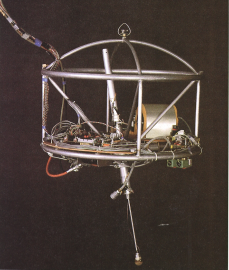
\includegraphics[width=\linewidth]{Figures/Hopper}
		\caption{One legged robot \cite{Raibert:1986:LR:5948.5950}}
		\label{fig:onlegg}
	\end{subfigure}\hfill
	\begin{subfigure}[b]{0.22\textwidth}
		\centering
		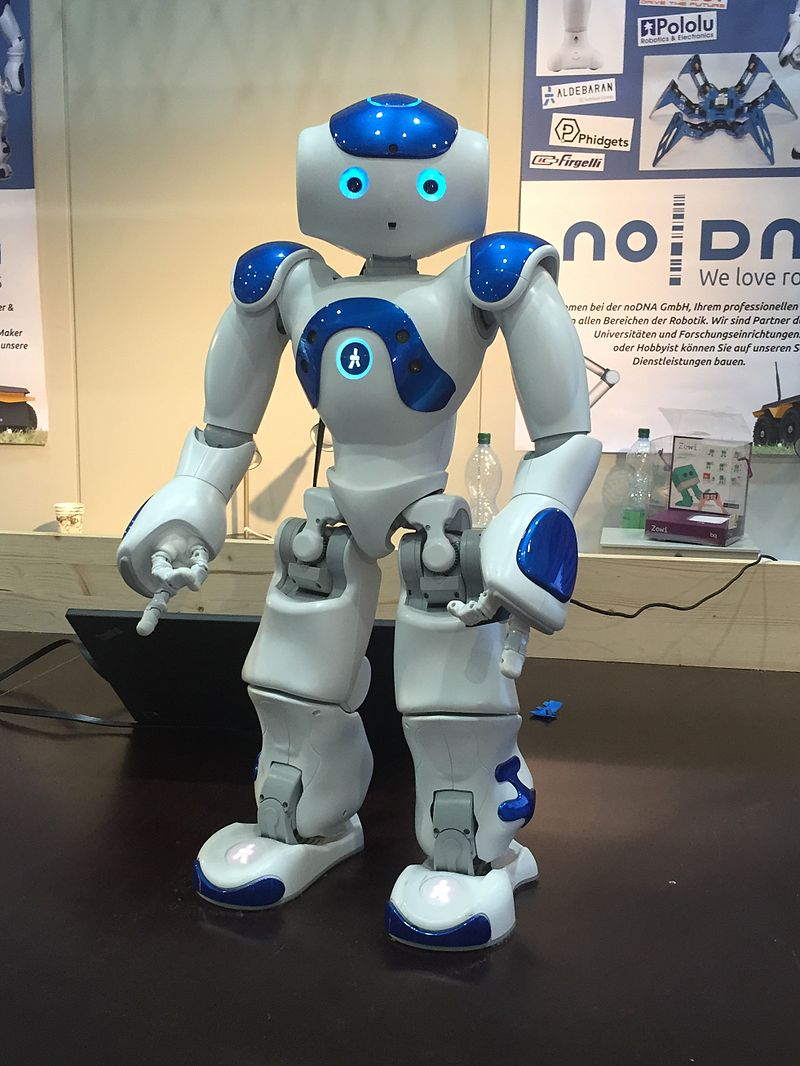
\includegraphics[width=\linewidth]{Figures/Nao_Robot}
		\caption{The NAO robot \cite{NAOImage}}
		\label{fig:nao}
	\end{subfigure}\hfill
	\begin{subfigure}[b]{0.22\textwidth}
		\centering
		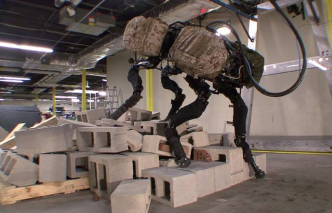
\includegraphics[width=\linewidth]{Figures/BigDog}
		\caption{The bigdog \cite{Raibert200810822}.}
		\label{fig:bigDog}
	\end{subfigure}\hfill
	\begin{subfigure}[b]{0.22\textwidth}
		\centering
		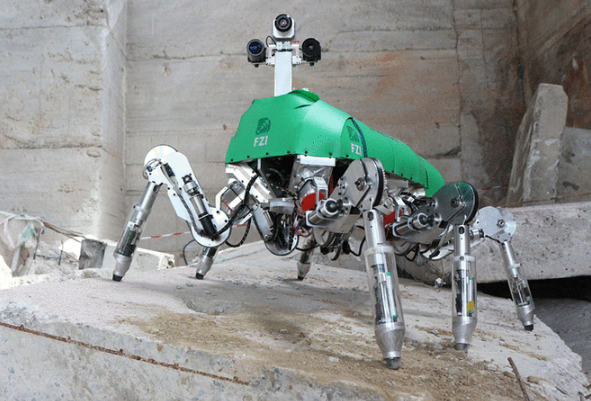
\includegraphics[width=\linewidth]{Figures/Lauron}
		\caption{Lauron V robot \cite{6878051}.}
		\label{fig:LAURON}
	\end{subfigure}
	\caption{Figure showing different types of legged robot.}\label{fig:robots}
\end{figure}

\FloatBarrier


\section{Tactile sensor}
Tactile sensor are designed for measure properties through direct physical interaction \cite{Cutkosky2008}. The tactile sensing provide many types of information which is can be obtained:

\begin{itemize}
	\item \textbf{Contact} is the most simple obtained from the sensor, which can detect touch from external agents. Further, one might want to measure the force of the contact. Once the sensor is able  
	\item \textbf{Force} provide amount of locally applied force.
	\item \textbf{Geometrical information} has the possibility to give geometrical shape the contact area, and also possible to deduce type of object, for instance sphere or cylinder.
	\item \textbf{Mechanical properties} such as slip condition, thermal or roughness.
\end{itemize}

Based on these information from tactile make it possibility of using it as manipulation, exploration or response. These activities is shown in figure \ref{fig:tactiles}. For manipulation it means that it is possible to control for instance the grip force on an object. The exploration has possibility of identify objects by assimilate information properties such as hardness, friction, and roughness from materials and surface. Response refer to detection and reaction to contacts from external agents, which could be sense if it was a gentle touch or impact.  


	\begin{figure}
	\centering
	\begin{subfigure}[b]{0.32\textwidth}
		\centering
		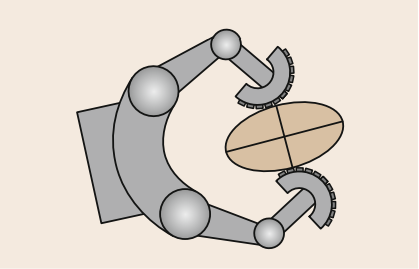
\includegraphics[width=\linewidth]{Figures/tactiles1}
		\caption{Manipulation}
		\label{fig:tact1}
	\end{subfigure}\hfill
	\begin{subfigure}[b]{0.32\textwidth}
		\centering
		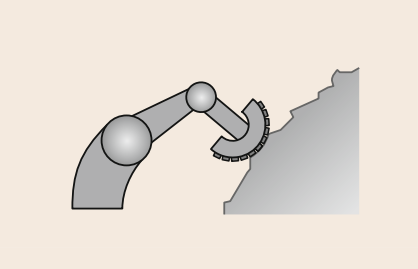
\includegraphics[width=\linewidth]{Figures/tactiles2}
		\caption{Exploration}
		\label{fig:tact2}
	\end{subfigure}\hfill
	\begin{subfigure}[b]{0.32\textwidth}
		\centering
		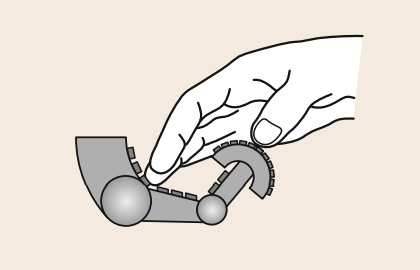
\includegraphics[width=\linewidth]{Figures/tactiles3}
		\caption{Response}
		\label{fig:tact3}
	\end{subfigure}\hfill
	\caption{Figures showing three types of application by using the tactile sensor \cite{Cutkosky2008}.}
	\label{fig:tactiles}
\end{figure}

\FloatBarrier


\section{Optical tactile force sensor}
Optical force sensor use light reflecting based on physical principle of light waves to measure the force. Some of the first optical tactile sensors \cite{220165,Nicholls1990} consist of an optical waveguide, made of transparent glass, which is illuminated along its edge by a light source, and use camera to analysis the images. These approaches are uniaxial, that is the sensor only capable of measure the force applied, but not the force direction. Ohka et al. \cite{525384}, modified and improved the technology and is popular construction of a three-axis tactile sensor and further optimized \cite{572232,ohka_mitsuya_matsunaga_takeuchi_2004,1545264}. The developed optical sensor consists of a charge-coupled device (CDD) camera, a light source, an acrylic hemispherical dome, and an array of rubber sensing elements. It shown promising result, when the sensor can identify differences of tribological behaviors between abrasive paper and a Teflon surface. Cameras have been widley used to capture deformation of a surface cause by external force \cite{1381228,7559098}
\\
\\
Another design and very common technology is based on Fiber Bragg Gratings (FBG) \cite{Heo2006312}. The FBG sensors are suitable for distributed strain monitoring, and offer advantages such as relative measurement and linear response. By exploiting the relationship between the variation of the external force and the FBG wavelength applied, the force can be measured.
\\
\\ 
An alternative to low cost 3-axis optical sensor is presented by Tar and Cserey \cite{6027100}, by using optoelectronic components. The design of the sensor consists of a hollow compliant convex surface made of silicone rubber, three photodiodes and an infra LED based sensor.  If a force is applied to the silicone rubber, it will cause a deformation that change the amount of light to each of photodiodes, which will change their force vector accordingly. Using the optical method to measure has offered highly dynamic sensory range, low noise, and high speed operation.
%http://ieeexplore.ieee.org/stamp/stamp.jsp?tp=&arnumber=7559098
%the light power variation is due to the variation of both the angle of view and the length of the optical path between the optoelectronic components
\\
\\
Another interesting approach use three sets of optical sensor to develop a 6-axial force sensor by Hirose and Yoneda \cite{125944}. The design of the sensor is cylindrical and contains three photosensors which measure the force around the cylinder. Another design of 6-axial optical force sensor can be found in \cite{6907805,6290303}.

%http://download.springer.com/static/pdf/934/bok%253A978-3-319-27340-2.pdf?originUrl=http%3A%2F%2Flink.springer.com%2Fbook%2F10.1007%2F978-3-319-27340-2&token2=exp=1492951378~acl=%2Fstatic%2Fpdf%2F934%2Fbok%25253A978-3-319-27340-2.pdf%3ForiginUrl%3Dhttp%253A%252F%252Flink.springer.com%252Fbook%252F10.1007%252F978-3-319-27340-2*~hmac=6e881e187a3cc0e1e04f4aabdf3f48393795889f42c9942e87077771bb132d4e


\section {Machine learning}
Machine learning is a type of artificial intelligence where it can learn to adapt or predict from earlier dataset without being explicitly programmed to do so. Each dataset consists of an feature vector which belong to a specified class. The training process consists of analyzing each feature vector and producing an inferred function, which is used for comparing new and unseen dataset to a class. The learning algorithm can be separated into supervised, unsupervised, reinforcement and evolutionary learning \cite{Marsland:2009:MLA:1571643}.

\paragraph{Supervised learning}
Supervised learning algorithms predict new data based on a labeled dataset. That is, the system in learning process known correct answers to each dataset, and will base the prediction on that. The learning process usually stops when the algorithm converge towards an acceptable level of performance.
	
\paragraph{Unsupervised learning}
Unsupervised learning algorithms make predictions from data points without label. The system has to organize the data on its own and make prediction based on that. A common method to organize the data is by clustering.
	
\paragraph{Reinforcement learning}
Reinforcement learning algorithms will choose an action to each dataset and it will receive a reward indicating how good the decision was. Based on rewards, the algorithms modifies its strategy in order to get the highest reward. 
	
\paragraph{Evolutionary learning}
Evolutionary learning use biological evolution such as reproduction, mutation, recombination, and selection as a learning process. 
	
 \subsection{Classifier} \label{sub:classifier}
The classifier is where the learning process occur, and produceS the inferred function. The following sections will introduce technical background of five classifiers; artifical neural network, support vector machine, Naive Bayes, k-nearest neighbors and decision tree.

\subsubsection{Artificial neural networks}
Artificial neural networks (ANN) is inspired by neurons in the human brain, and is one of the most popular learning algorithms. It can be found in many different research fields, such as signal processing, image processing, natural language processing etc. A common representation of a neuron is the perceptron shown in figure \ref{fig:NN}. It consists a set of weighted inputs $w_i$, an adder which sums weighted inputs signals, and an activation function to decide whether it should fire for the current input $x_i$. By connecting many perceptrons, one will obtain a neural network. Note that neurons only dependent on its inputs and error. That is, a neuron will not be affected by other neurons performance. Each neuron gives a result based on its own weights and the input, adding them together, and comparing the result to its own threshold. The only thing neurons share is the input. 
\\
\\
The learning process of a perceptron in supervised learning is to be able to reproduce a particular pattern to a class, which consist of firing and non-firing neurons for a given input. If some of the neurons yield a wrong output, for instance a neuron did not fire when it should, then its weights will be adjusted to make it fire right the next time. There is a possible to add more layers to the neural network, which make it able to handle non linearly separable problems. This is also called multi-layer perceptron (MLP), or multi neural network.

	
\begin{figure}[h]
	\centering
	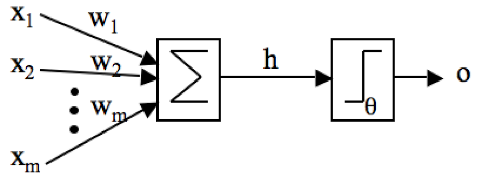
\includegraphics[scale=0.9]{Figures/neuron2.PNG}
	\caption{Figure showing a simple model of a single perceptron \cite{Marsland:2009:MLA:1571643}}
	\label{fig:NN}
\end{figure}
	
\paragraph{Multi-Layer Perceptron}
A multi-layer perceptron consists of two or more layers between the input and output. Those layers are also called hidden layers because its value cannot be changed directly, and it is only observed in the training set. The training process can be divided into forward algorithm and backward algorithm. The forward algorithm start first by calculating the activations of the first hidden layer. Those activations and the next set of weights will be used to calculate the activations for the next layer, which could either be a hidden layer or the output. The output will then be compared to a target to compute an error. The backwards algorithm will be using the error to adjust the weights between the output-layer and hidden-layer. The algorithm stops when it has reach the inputs and changed weights in the entire graph.
	
	
\begin{figure}[h]
	\centering
	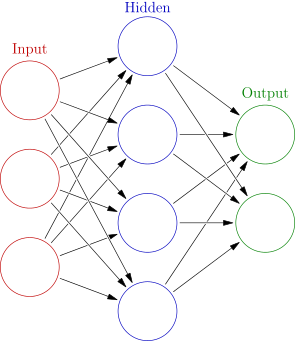
\includegraphics[scale=0.6]{Figures/MLP.png}
	\caption{Figure showing a multi-layer perceptron with 1 hidden layer \cite{MLP}. It is possible to increase the number of hidden layers and nodes to each layer}
	\label{fig:MLP}
\end{figure}
	
\subsubsection{Support vector machine}
Support vector machine (SVM) algorithm was introduced by Cortes and Vapnik \cite{Cortes1995}, and the  classifier often provide significantly better performance than other algorithms, when the data set is not extremely large \cite{Marsland:2009:MLA:1571643}. An instance of two-class classification is shown in figure \ref{fig:SVM}. Each of features vector with values according to the x- and y-axis, represents as classes: circles and crosses. The dotted line is the hyperplane/decision boundary and tells where each class belongs to. The SVM will create an optimal hyperplane to achieve the best separation between classes. If the decision boundary was moved with small amount, it has a risk that a datapoint from one class that lies close to the boundary, be on the wrong side. To find the best decision boundary is by defining the optimal margin. The margin is defined as the largest region it can put that separate the classes without having any points inside. The hatched classes lies on the margin, and support vectors. This can process can be done by the dot product between each datapoints \cite{Cortes1995}.
	
\begin{figure}[h]
	\centering
	%    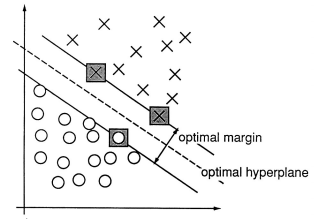
\includegraphics[width=\textwidth,height=\textheight,keepaspectratio]{Figures/SVM.PNG}
	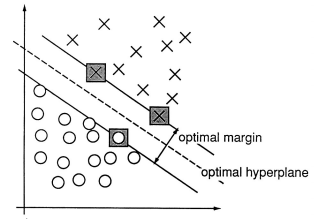
\includegraphics{Figures/SVM.PNG}
	\caption{Figure showing an example of a optimal hyperplane create by SVM on a two-class classification problem  \cite{Cortes1995}.}
	\label{fig:SVM}
\end{figure}
\FloatBarrier

A weakness of the SVM, is only feasible when the classes are linearly separable as shown in \ref{fig:SVM}. However, this issue is prevented by transforming the data into a higher dimensional space where the data is linearly separable, as shown in figure \ref{fig:svmtransform}. Recall that the decision boundary is only dependent on the dot-product of each datapoints, which means the transformation itself is not needed, but instead, using a function to that implicitly computes the high-dimensional dot-product, and is referred as the kernel function.
	
\begin{figure}[h]
	\centering
	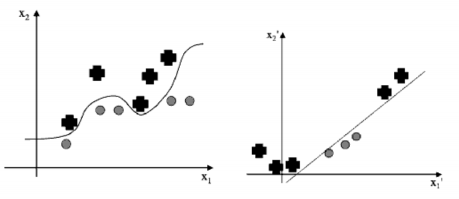
\includegraphics{Figures/svmtransform}
	\caption{Figure showing transformation of the data from non linearly separable to linearly separable space \cite{Marsland:2009:MLA:1571643}.}
	\label{fig:svmtransform}
\end{figure}
\FloatBarrier
	
\subsubsection{Naive bayes}
Naive Bayes algorithm is a probabilistic classifier based on Bayes’ theorem with the assumption that the effect of a feature on a given class is independent of the values of other variables \cite{Marsland:2009:MLA:1571643}. The assumption simplify computation, and is the reason to be considered as naive. Consider a vector with n features, $X_j$, and a class, $C_i$, then the Bayes theorem can be formulated equation \ref{eq:bayesNaivews2}.
\begin{equation} 
P(C_i \vert X_j) = \frac{P(X_j \vert C_i)P(C_i)}{P(X_j)}
\label{eq:bayesNaivews2}
\end{equation}
The given output, $P(C_i \vert X_j)$, is the probability that the features $X_j$, belongs to a class $C_i$, while $P(X_j \vert C_i)$, is the probability of the class $C_i$, belongs with this set of features $X_j$.  $P(C_i)$ and $P(X_j)$ are the prior probability of $C_i$ and  $X_j$ respectively. The problem of using the Bayes theorem occur, when the number of features increase, which require more computation time. Thus, with assumptions of independence, the equation \ref{eq:bayesNaivews2} can be reformulated as equation \ref{eq:naiveB}.
\begin{equation} 
P(C_i \vert X_j)  = P(C_i)\prod_{k}P(X_{j}^{k} \vert C_i)
\label{eq:naiveB}
\end{equation}
Prediction is based by selecting the class $C_i$, with the highest probability. 

\subsubsection{K-nearest neighbors}
K-nearest neighbors (KNN) is one of the simple classifiers presented by Cover and Hart \cite{1053964}. The classification process consists of looking at the k-nearest classes and classify the new data as the class with biggest majority among them. Choosing the value for k will therefore be crucial to achieve high classification accuracy. An example to illustrate effect of performance on different k values is shown \ref{fig:KNN}. All the blue squares and red triangles are the training data, while the green circle represent new data, which is to be classified. The solid and dashed circle is when the k is set to either 3 or 5 respectively, and illustrate the boundary between k nearest among all classes. If k is set to 3, the green circle will be classified as triangle, which is the majority among them. However, if k is set to 5, then the green circle will be classified as square.



\begin{figure}[h]
		\centering
		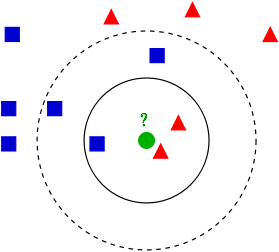
\includegraphics[scale=0.5]{Figures/KNN.png}
		\caption{Figure showing an example of a KNN classification \cite{KnnClassification}. The green circle is to be classified to either blue square or red triangle. The solid circle is when k = 3, while the dashed circle is when k = 5.}
		\label{fig:KNN}
\end{figure}
	
A commonly method to find the k-nearest datapoint is to calculate the Euclidean Distance. The euclidean distance can be expressed as shown in equation\ref{eq:edistance} \cite{Bao2004}.
	
\begin{equation}
	D(x,y)=\sqrt{\sum_{i=1}^{m}(x_{i}-y_{i})^2}
	\label{eq:edistance}
\end{equation}

The x and y in equation \ref{eq:edistance} represent the actual and unseen class, and m is the number of features to each of classes in x and y. The algorithm will then count the k classes with shortest distance to determine which class the unseen data belongs to.
	
	
\subsubsection{Decision tree}
The decision tree is a non-parametric classifier presented by JR Quinlan \cite{Quinlan1986}. A tree consists of nodes, which represent one of the features, and leaf nodes are associated with classes. The process of the decision tree is constructing a tree consisting of nodes and edges, and predict by following a path from the root to a leaf node. In figure \ref{fig:decisiontree} shows an example of a decision tree.


	
\begin{figure}[h]
		\centering
		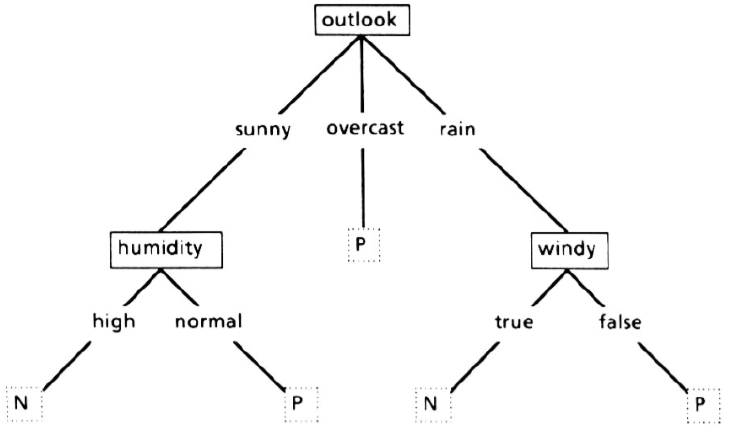
\includegraphics[scale=0.5]{Figures/decisionTree.PNG}
		\caption{Figure showing an example of a simple decision tree \cite{Quinlan1986}. This decision tree classify a day to be P or N based on outlook, humidity and windy.}
		\label{fig:decisiontree}
\end{figure}
\FloatBarrier

An important aspect of decision trees is how to construct one, based on the features. Although there are few different methods, mostly are based on same principle, by starting at the root, and chose the most discriminative feature at each step \cite{Marsland:2009:MLA:1571643}. The attractiveness with trees, are efficient, and easy to understand and interpret the data. 

\subsection{Hyperparameter tuning}
Every classifier has parameters that need to be set and may strongly affect the performance induced by them. Thus, to optimize a classifier, it is recommended to finding these appropriate parameters. It is difficult to know optimal values of parameters, since it often differ for different datasets. A strategy to finding these parameters recommended by Hsu et al. \cite{Hsu10apractical}, is using a grid search. Grid search will exhaustive search through a desired specified subset and output the parameters with best results. Benefit of using grid search instead of search by heuristics or approximations, is it avoid get stuck in local optima. However, the biggest weakness is computation complexity when the search space increase. 


\section{Features} \label{features}
An important part of achieving a good classification, is finding good features from sensor data. The features is what distinguish between classes and will be used as learning set. Thus, finding good features is crucial to achieve a accurate classifier.
	
\subsection{Curse of dimensionality}\label{curseDim}
The curse of dimensionality occurs when one include too many features to the input vector. When the dimensionality of features vector increase, the complexity of underlying pattern might increase and the performance of the classifier will be degrade. To prevent the curse of dimensionality one can add more samples to uncover the underlying pattern.
	
\subsection{Features extraction} \label{feature_extraction}
Feature extraction is the process to build a new set of features from the original set and use it as training set. Those extracted features should make it easy for a classifier to distinguish between the various classes. A common method is extracting statistical features.
	
\subsubsection{Statistical features} \label{sub:statical}
The following paragraphs will be explaining five commonly used statical features; mean, variance, standard deviation, skewness and kurtosis.
	
\paragraph{Mean}
The mean is generally referred to the average, and is defined as sum of the values divided by the number of values\cite{Press:2007:NRE:1403886}:
	
\begin{equation}
\bar{x} = \frac{1}{N}\sum_{N-1}^{j=0}x_{j}
\label{eq:mean}
\end{equation}
	
	
\paragraph{Variance}
Variance describe the spread between numbers in a data set. The variance can be written as\cite{Press:2007:NRE:1403886}:
	
	\begin{equation}
	Var(x_0\dotsc X_{N-1})  = \frac{1}{N}\sum_{N-1}^{j=0}(x_{j}-\bar{x})^2
	\label{eq:variance}
	\end{equation}

\paragraph{Standard deviation}
Standard deviation is a measure of spread of a data set from its mean. High deviation indicate that the data points are further from the mean. This can be calculated by taking the square root from variance\cite{Press:2007:NRE:1403886}:
	
	\begin{equation}
	\sigma(x_0\dotsc X_{N-1})  = \sqrt{Var(x_0\dotsc X_{N-1})}
	\label{eq:std}
	\end{equation}
	
\paragraph{Skewness} 
Skewness describes asymmetry of a distribution. The formula is\cite{Press:2007:NRE:1403886}:
	\begin{equation}
	Skew(x_0\dotsc X_{N-1})  =  \frac{1}{N}\sum_{N-1}^{j=0}\left [ \frac{x_j-\bar{x}}{\sigma} \right ]^3
	\label{eq:skew}
	\end{equation}
	
The skewness can be either negative or positive depending on whether data points are skewed to the left or to the right. If data is skewed to the left indicate a negative skewness, while positive skewness is when the data is skewed to the right. An illustration of both positive and negative skewness is shown in figure \ref{fig:skew}.
	
	\begin{figure}[h]
		\centering
		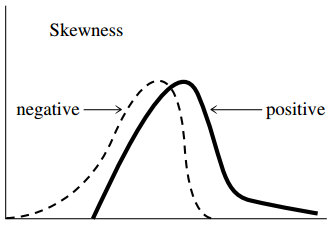
\includegraphics[scale=0.8]{Figures/Skewness}
		\caption{Skewness \cite{Press:2007:NRE:1403886}}
		\label{fig:skew}
	\end{figure}
	
	\FloatBarrier
	
\paragraph{Kurtosis}
Kurtosis measure the peak and tails of a distribution relative to a normal distribution. Using kurtosis might help to understand general characteristics about the distribution of the data. The formula is\cite{Press:2007:NRE:1403886}:
	\begin{equation}
	Kurt(x_0\dotsc X_{N-1}) = \left \{ \frac{1}{N}\sum_{N-1}^{j=0}\left [ \frac{x_j-\bar{x}}{\sigma} \right ]^4 \right \}-3
	\label{eq:kurtosis}
	\end{equation}
	
A positive kurtosis of a distribution has a sharper peak and heavier tails relative to normal distribution. While a negative kurtosis has flatter peak and lighter tails relative to normal distribution. An illustration of both positive and negative kurtosis is shown in figure \ref{fig:kurtosis}
	
	
	\begin{figure}[h]
		\centering
		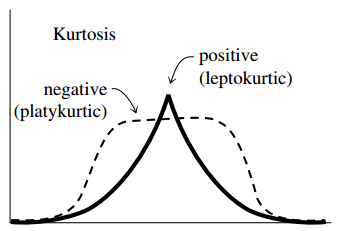
\includegraphics[scale=0.8]{Figures/Kurtosis}
		\caption{Kurtosis \cite{Press:2007:NRE:1403886}}
		\label{fig:kurtosis}
	\end{figure}
	
	%http://greenteapress.com/thinkstats/thinkstats.pdf
	
	%\paragraph{Time domain}
	%\paragraph{Fourier transform}
	
	
\subsection{Features selection}\label{selection}	
The process in feature selection is to select a subset of features from the original set. Selecting good features has benefit of increasing classifier performance, prevent the curse of dimensionality mentioned in section \ref{curseDim} and reducing storage requirements and training time. Note that a features can individually be completely useless, but relevant when used together with other features \cite{Guyon2006}. There are three types of feature selection algorithms: filter-, wrapper- and embedded methods. %as shown in figure \ref{fig:selection}. 
	

\begin{comment}
	\begin{figure}[h]
		\centering
		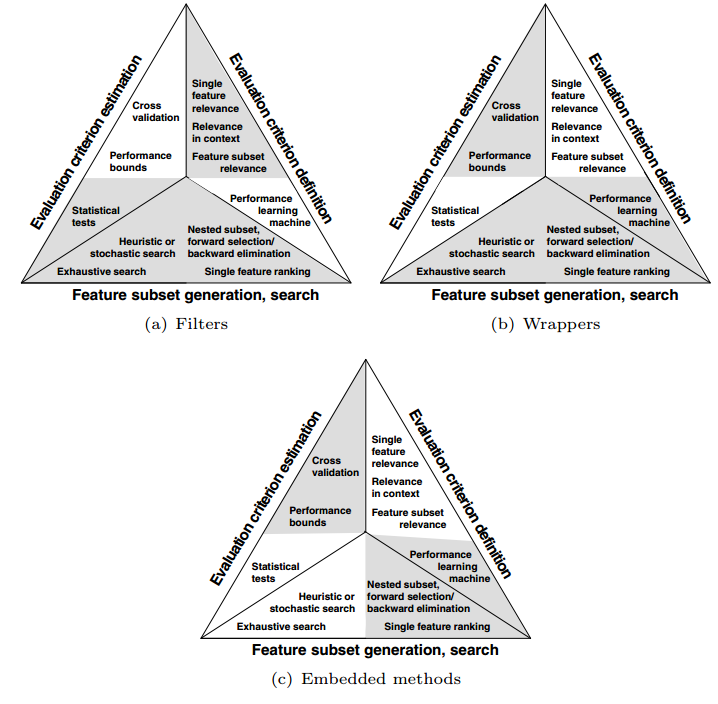
\includegraphics[scale=0.7]{Figures/FilterWrapperEmbedded.PNG}
		\caption{The figure showing the three approaches of feature selection \cite{Guyon2006}. (a) filter method (b) wrapper method and (c) embedded method.  The shades show the components used by the three methods.}
		\label{fig:selection}
	\end{figure}
\end{comment}
	
	
\paragraph{Filter}
Filter feature selection is independent of any classifier. It uses statistical measures to assign each feature a score. Features will either be kept or removed based on the score. The filter methods are considered fast and effective, specially when the number of features is large and the number of available training examples comparatively small.  
	
	
\paragraph{Wrapper}
Wrapper feature selection will try different combination of the feature set, evaluate by a classifier and keep the feature set with best result.
	
	
\paragraph{Embedded}
Embedded feature selection perform feature selection as part of the learning procedure and are usually specific to given classifier.

\subsection{Features scaling} \label{subsec:scaling}
To reduce bias effect cause by skewed distributions, it is common to standardize the feature vectors. Classifiers such as SVM and KNN described in section \ref{sub:classifier}, involve distances in their computation, might cause poor performance when one of the vector has a large range, then it will dominate other attributes.

	
\section{Model validation}
Model validation relate to evaluate the performance of a classifier. 
	
\subsection{No free lunch theorem} \label{seq:nofree}
The well-known no free lunch theorem\cite{NOFREELUNCH} in machine learning states that there is no best classifier for every problem. That is, even if a model achieve great performance for one problem, might not hold for another problem. Thus, it is recommended to apply several classifier.
	
\subsection{Ovefitting and underfitting}
Overfitting and underfitting the data is a issue in machine learning which cause a poor performance of classification. Overfitting occurs if there are too many training data or if it has adapted to the noise within data set. While underfitting occurs if there are not enough training data and will not be able to generalize new data set. An example for each case is shown in figure \ref{fig:fitting}. The cross-validation estimate how accurately the classifier model will perform in practice, which might prevent overfitting or underfitting the data.

	\begin{figure}[h]
		\begin{subfigure}{0.5\linewidth}
			\centering
			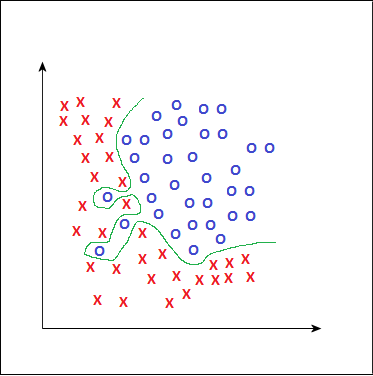
\includegraphics[scale=0.43]{Figures/Overfitting}
			\caption{Overfitting}
			\label{fig:over}
		\end{subfigure}%
		\begin{subfigure}{.5\linewidth}
			\centering
			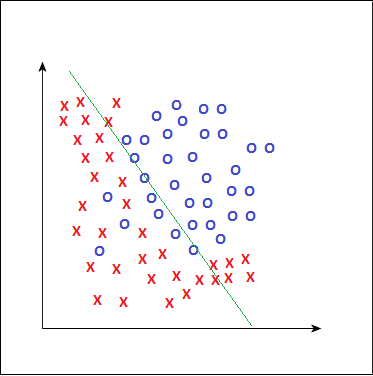
\includegraphics[scale=0.43]{Figures/Underfitting}
			\caption{Underfitting}
			\label{fig:under}
		\end{subfigure}\\[1ex]
		\begin{subfigure}{\linewidth}
			\centering
			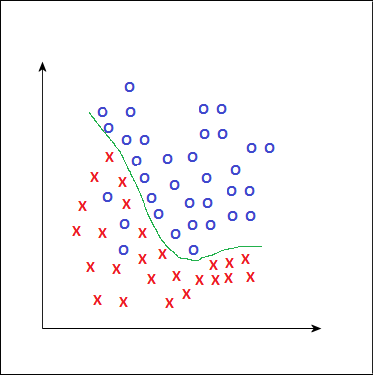
\includegraphics[scale=0.43]{Figures/Finefitting}
			\caption{Optimal}
			\label{fig:optimal}
		\end{subfigure}
		\caption{Figur illustrate when a model is \ref{fig:over} overfitted, \ref{fig:under} underfitted and \ref{fig:optimal}optimal }
		\label{fig:fitting}	
	\end{figure}
	
	\FloatBarrier
	
\subsection{Cross-Validation}
Cross-validation is a statistical method to assess the quality and comparing learning models \cite{Refaeilzadeh2009}. The process of cross-validation is to first remove some of the data before the training begins. After the training, it will use the removed data to test the performance. The intention is to evaluate the classifier performance in more realistic scenario by predicting new and unseen data. The K-fold is a common cross-validation method.
	
\paragraph{K-fold}
The process of k-fold is to partitioned the data into k subset, where one subset is used for testing and the other are used for training. When the trained model has assessed the test set, a new subset is selected as test set. This process is repeated k times, that is when all subsets have been used as a test set. Setting k to the length of feature vectors is also know as leave-one-out cross-validation (LOOCV). LOOCV only use one feature vector as test set, while the rest as training set shown in figure \ref{fig:kfold}. Estimation based on LOOCV tend to be almost unbiased, but unreliable
estimate due to high variance. However, the advantages is that use as many training samples as possible and is widely used especially when the there are only  small amount of data available. 
 	
	\begin{figure}[h]
		\centering
		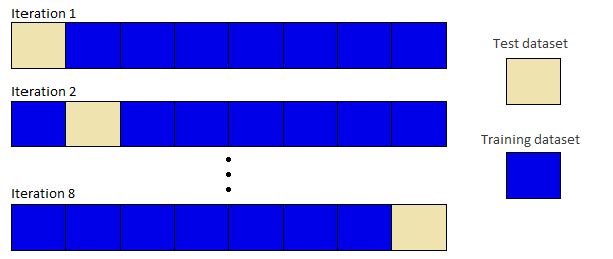
\includegraphics[scale=0.6]{Figures/Kfold}
		\caption{The figure showing an instance of k-fold cross validation. In this case the k is set to be 8 which is also the length of feature vectors}
		\label{fig:kfold}
	\end{figure}
	
	%Se: Rigidity-based surface recognition for a domestic legged robot.
	
	
\subsection{Evaluating Classifiers}\label{subsec:evalclf}
Evaluation of the performance to classifier can be done by calculate metrics based on correct or wrong output. For instance a two-class classifier with classes, "postive" and "negative" will have four different outcomes:
	
	\begin{enumerate}
		\item True postive (TP) is correct prediction of class positive
		\item True negative (TN) is correct prediction of class negative
		\item False positive (FP) is wrong prediction of class positive
		\item False negative (FN) is wrong prediction of class positive
	\end{enumerate}
	
	Those four variables can be further used to calculate the precision, accuracy, recall and f-score.
	
	\paragraph{Precision}
	Precision gives the number of correct detected class members.
	\begin{equation}
	Precision = \frac{TP}{TP + FP}
	\label{eq:prec}
	\end{equation}
	
	\paragraph{Accuracy}
	Accuracy gives the ratio of correct prediction. 
	\begin{equation}
	Accuracy = \frac{TP + TN}{TP + TN + FP + FN}
	\label{eq:acc}
	\end{equation}
	
	\paragraph{Recall}
	Recall gives the number of detected actual class members.
	
	\begin{equation}
	Recall = \frac{TP}{TP + FN}
	\label{eq:recall}
	\end{equation}
	
	\paragraph{F-score}
	F-score is a balanced measure of recall and precision 
	\begin{equation}
	\textit{F-score} = 2*\frac{Precision*Recall}{Precision + Recall}
	\label{eq:fscore}
	\end{equation}
	%\part{The project}                    %% ... or ??
	\FloatBarrier
The accuracy will tell the overall performance of the model. However, there is a possibility that the model only classify three of four terrains correctly and still get a high accuracy. Thus, it will be recommended to look at the f-score. A low f-score indicate that the class either has a low precision, recall or both. Low precision indicate that the classifier has difficulty to predict the currently class, while low recall indicate that is more likely that a class is to be classified in other classes.
\\
\\
It will be interesting to see which of class was easier to predict than others. This can be seen by using confusion matrix. The confusion matrix consists a square matrix with one row for predicted class, and and column for actual class (or vice-versa).
An example of confusion matrix is shown on table \ref{tab:cmatrix}
	
	\begin{table}[h]
		\centering
		\begin{tabular}{ll|l|l|l|}
			\cline{3-5}
			&  & \multicolumn{3}{c|}{Actual} \\ \cline{3-5} 
			&  & $C_1$ & $C_2$ & $C_3$ \\ \hline
			\multicolumn{1}{|l|}{\multirow{3}{*}{Predicted}} & $C_1$ & 8 & 0 & 0 \\ \cline{2-5} 
			\multicolumn{1}{|l|}{} & $C_2$ & 5 & 8 & 1 \\ \cline{2-5} 
			\multicolumn{1}{|l|}{} & $C_3$ & 5 & 3 & 8 \\ \hline
		\end{tabular}
		\caption{A confusion matrix of 3-class classification.}
		\label{tab:cmatrix}
	\end{table}
	
	
\section{Existing work on terrain classification}
The terrain classification has been applied to both wheeled and legged robots. Wheeled robots have the benefit of achieving stable locomotion by changing their speed on different terrains, while the legged robots must either change their gait, walking speed or both. Changing the gait for a legged robot can be complex, but has the benefit of traverse on more difficult terrains. 
\\
\\
The most commonly used legged robot in terrain classification is using quadruped \cite{6784609,littleDog,6849778,Hoffmann20141790} and hexapod \cite{Walas2015,26b23e912c654fe4b7478fd910130195,6569179}, due to its stability on rough terrain. However a few has used one legged robot \cite{5602459}. Biped for terrain classification is still unsuitable since it is hard to maintain stability on rough terrain.
\\
\\
The bayes theorem suit to mathematical express the terrain identification problem, and allow to evaluate unexpected mismatch between sample classes and the real environments. In equation \ref{eq:bayesNaivews2}, the A could represent possible terrains that is expected to predict, while B is the data from sensor. According to the equation \ref{eq:bayesNaivews2} the $P(A \vert B)$ will be the likelihood that the terrain is this with these data from senor.

	%http://e-collection.library.ethz.ch/eserv/eth:7893/eth-7893-02.pdf#search=%22terrain classification%22
	%file:///C:/Users/Jay/Downloads/Paper_MME_2006_JATMachado_MFSilva%20(2).pdf
	%http://www.robotplatform.com/knowledge/Classification_of_Robots/legged_robots.html
	%http://www2.cs.siu.edu/~hexmoor/classes/CS404-S09/RobotLocomotion.pdf
	%http://www.idt.mdh.se/kurser/ct3340/ht12/MINICONFERENCE/FinalPapers/ircse12_submission_21.pdf
		
\subsection{Importance of terrain classification}
The importance of terrain classification for legged robots is that the terrain has a major factor affecting the decision for the gait change \cite{6569179}. Most of the legged robot has the benefit of changing their gait and walking speed to achieve a stable locomotion. For instance a running gait can be efficient on flat road, but fail to maintain the stability when used on ice, cause of slipping. An example of application is shown in Giguere et al. \cite{Giguere06environmentidentification}, where a amphibious legged robot can switch from walking to swimming gait, according to which of the terrain it is on. 
\\
\\
It has been shown that different controllers were suited for different terrain by letting quadrupedal robot hopping on soft and hard terrain \cite{7487541}. Other has investigated the effect of performance with different gaits parameters on different terrains \cite{6569179}. Some of the result showed that the energy consumption and the walking speed is tied to the terrain type. That is, a trade-off between the physical speed and the power consumption of the robot can be achieved by controlling the cycle-frequency of the leg rotation.
	
	
\subsection{Terrain sensing}
In order to classify various of terrains, the system must obtain information from the terrain either by remote sensing, local sensing or both.
	
\paragraph{Remote sensing}
The remote sensing obtain information of a terrain from a distance and do not measure the terrain physically. The camera is most widely used and discriminating the terrain is based on analyzing images.
\\
\\ 
Filitchkin et al. \cite{littleDog} presents an visual terrain classification by using a single, compact camera to change the gait patterns of a quadruped robot. Three types of gaits were used during the experiment, a gait designed for flat surface, a gait for rough terrain and a mixture of the two first. To know which gait should be chosen for each terrain, an initial test by assigning a gait to each terrain type is required. There were totally four different terrain: small rocks, rocks, grass and tile. Lastly, the experiment was let the robot execute a terrain classification cycle every few steps and switched to one of three gait according which terrain it is on. Robot performance was measured by comparing the traversal time between for each three gait and the changing gait. The result shown that the changing gait is able to terrain classification and traverse through the terrain faster. The other two gait were fast, but was not able to classify big rocks, while the last gait was able to classify all terrain but had slower traverse time.
\\
\\
Plagemann et al. \cite{4651026} used laser ranger finder to predict terrain elevation at unseen locations.
The researches extended the Gaussian process model to achieve a more accurate prediction of elevations. The result show that the proposed method is capable of accurately predicting elevations in the presence of noise even at unobserved locations. These features allowed them to plan foot trajectories of the robot to reach the goal location. 
\\
\\
A weakness of using the remote sensors, is that it does not give insight into the characteristic of currently terrain. For instance remote sensor might has difficulties to distinguish between a terrain that is covered with either compacted or uncompacted snow. An another option to measure terrain directly is by local sensing. 
	
\paragraph{Local sensing}
Local sensing measure aspects of the interaction between the robot and terrain as the robot walk through. This gives a measurement of mechanical terrain properties and provide useful information such as how the environment is affecting currently robot performance. 
\\
\\ 
Stejskal et al. \cite{7487544} present a road following hexapod robot by using the feedback from robot servo drives. The road following consists of let the robot blindly walk on road. After each gait cycle, the robot will determines whether it is on new terrain or on road. If it is determined as off road, then the robot will steer back to the road. Data from the servo provides information about the leg motion which were position error, current speed and torque. Three different terrains, asphalt, dirt and grass were used during the experiment. The robot was most confused by dirt, which had about 86\% of misclassified samples. The author states that the transition from asphalt to dirt was usually flat, which means that the leg motion of walking on flat dirt has a similar leg motion as walking on asphalt. Beside of that, the overall result of terrain classification had an accuracy of 96.2\%, which can be considered as feasible approach and data from leg motion keeps the robot on the road.
\\
\\
Kim et al. \cite{5602459} used the ground reaction force and torque sensors of an one-legged robot due to terrain classification. The goal of the research was to compare the performance between neural network and support vector machine. Four different terrains were used in the experiments which were flat, grass, sand, and gravel. The data were collected by walking through each terrain many times. Different features were extracted from the data, and partitioned into a training and test set. The result shown the support vector machine got an accuracy on 78.75\%, which performed slightly better than neural network on 78.6\%.
\\
\\
Hoepflinger et al. \cite{5509309} present a novel approach to terrain classification for legged robots by using properties from joint motor currents and force sensing resistor. The goal was to improve the guiding of foot placement and stability of legged robots in rough terrain. Usually experiments is done by having a robot walk through terrains. However in this experiment the author separated one of the legs robot and mounted to a sample holder of a testbed. The first experiment consist of distinguish four different shaped terrain: a convex and a concave cone, a convex hemispherical bulge, and a concave hemispherical indentation. The data were collected by the knee-joint oscillated slightly with an amplitude of approximately one degree on the terrain. In the second experiment was to distinguish between three different types surfaces such as abrasive paper and a low friction PTFE coating. Collecting of data were done by performing a scratching motion on the terrain. The result of terrain shape classification had a high success rate. Convex cone and concave cone had 100\% accuracy, while the concave hemisphere bulge 95\% and 80\% on for the convex hemispherical bulge. Regarding surface classification show that the algorithm performed slightly worse. A type of an abrasive paper had a accuracy of 53.3\%. Even a low accuracy the author state it is overall an satisfy result, since the average correct prediction of different types of abrasive paper was two of three, and prediction of teflon coated surface had an high accuracy 93.3\%.
\\
\\
Other examples of terrain classification can be found in \cite{Giguere2009,6386243,6569179,6569179,4399500}.
	
\subsection{Learning algorithms}
There is a vast number of classifiers and various has been used within the terrain classification such as neural network \cite{6784609,5752869,4654717}, adaptive bayesian filtering \cite{5152327,6849778}, support vector machines \cite{5602459,4161556,4059113} and decision tree \cite{6849778}.
\\
\\
The no free lunch theorem described in section \ref{seq:nofree} can be seen in previous work has shown that SVM, KNN and naive bayes gave higher accuracy than the decision tree \cite{DBLP:conf/emcr/WeissFSZ07}, while in \cite{6849778} achieved a better performance on SVM, decision tree and naive bayes than KNN. It is therefore common to build several algorithms, and chose the best of them for the specified problem. 
\\
\\
Mostly study based their terrain classification on supervised learning. However, Giguere and Dudek \cite{Giguere2009} presented a new clustering method to terrain classification using unsupervised learning. This make a robot to be able automatically distinguish terrain without any human interaction or feedback. Another work of the same authors  \cite{5752869} made a tactile probe and demonstrated that it can be used in unsupervised learning.
	
\subsection{Features} \label{sub:relatedfeatures}
As mentioned in section \ref{features} finding good features is a crucial part of classification process. Earlier work has extracted features in combination of statistical features in the time domain with frequency domain features \cite{5152662} \cite{Giguere2009} \cite{5509309}. While others only use the frequency domain \cite{4543710} \cite{5979766}.
\\
\\
Giguere and Dudek \cite{5152662} extracted features such as mean, variance, skewness, kurtosis, fifth moment and sum of the variation over time in time domain. While in frequency domain where the sum of higher half of amplitude spectrum extracted.
\\
\\
Hoffmann el at. \cite{Hoffmann20141790} defined features in time domain such as, minimum, maximum, mean, kurtosis, skewness, median, standard deviation, approximation of the integral, amplitude of Hilbert transform. Other features was extracted in frequency domain such as frequency with highest amplitude and its magnitude, and similar to the second and third highest amplitude. 
\\
\\
Kertész \cite{7387710} computed median, maximum, skewness and root mean square from of the accelerometer angles in x, y and z-direction. Those features were also extracted in frequency domain for the z-direction. Features extracted from force sensors were interquartile range, maximum, skewness, RMS amplitude and the highest amplitude in frequency domain.
\\
\\
Best el at.\cite{26b23e912c654fe4b7478fd910130195} extracted five statistical features in domain such as minimum, maximum, mean median and standard deviation. However some of statistical features is also calculated in frequency domain with the energy additionally.
\\
\\
As it can be seen that many of the features is extracted by statistical features which is described in section \ref{sub:statical}. An example of extracting good features can be seen in \cite{5602459}. Using statistic with support vector machine gave an accuracy on 40\%, while principal component analysis gave an accuracy on 78.75\%. Note that the author only used variance, kurtosis and skewness as statistic features. 
	
\subsection{Validation}\label{subseq:validation}
A common method of validation is using the k-fold cross-validation \cite{DBLP:conf/itat/MrvaF15,6784609,6386243,Hoffmann20141790,6849778,7387710}. However the choice of selecting k vary. A common k value is to be set either two \cite{DBLP:conf/itat/MrvaF15,6784609}, 10 \cite{26b23e912c654fe4b7478fd910130195,6386243,Hoffmann20141790,6849778,7387710} or equal the length of feature vectors \cite{26b23e912c654fe4b7478fd910130195}.
\\
\\
Mrva et al. \cite{DBLP:conf/itat/MrvaF15} used 2-fold cross validation and achieved a overall accuracy 99.4\%, and states the possibility of obtaining 100\% with more folds. Best el at. \cite{26b23e912c654fe4b7478fd910130195} used 10-fold cross validation and achieved a high precision and recall for all five terrains, while leave-one-out-cross validation let the classifier being confused between grass and concrete terrains. 
\\
\\
As stated in \cite{7387710}, the k-fold gives a reasonable estimate of the performance, however, it does not tell how well it predict on unseen data. This is because the experiment always use same samples where it involve in either training or testing. The model might be less generalized, data are more likely referring to themselves and will have difficulty of predicting unseen data. Mostly authors is aware of the this and has rectified it by partitioned the samples to make the training and test set independent \cite{26b23e912c654fe4b7478fd910130195}. The learning process will only be used from a certain set, and test is from other set.
\\
\\
Not all studies evaluated their models by k-fold cross-validation, but either with new data to get a better estimation or real accuracy \cite{5509309,Walas2015,5752869}. A more simple method of validation is to randomly partition the data set with 70\% used for training, and the rest used for testing \cite{5752869}. The most realistic scenario is to base the evaluation by having a robot traversing through different terrains \cite{DBLP:conf/itat/MrvaF15}.


\chapter{Softwares and tools} \label{chap:software}
This chapter gives an introduction of different tools and libraries used throughout the thesis.


\section{Optical force sensor}
OptoForce (3D force sensor) \cite{Optoforce} is a similar sensor to Tar and Cserey \cite{6027100}, and the construction of the sensor is shown in the figure \ref{fig:OptoforceBuild}. 
\begin{figure}[h]
	\centering
	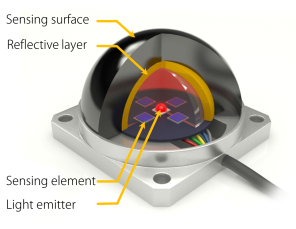
\includegraphics[scale=0.8]{Figures/OptoforceBuild}
	\caption{Figure showing construction of the 3d optical force used in thesis \cite{OptoforceFig}}
	\label{fig:OptoforceBuild}
\end{figure}
\FloatBarrier

The sensor consists of a light emitter (LED) and four sensing elements (photodiodes) which is wrapped within two layers; a reflective layer and a sensing surface. The four photodiodes obtain the force by measuring the infrared light reflected by the reflective layer. If a force is applied on the sensing surface, the amount of reflected light to each photodiodes will change accordingly. The forces in x- and y-direction are measured from the difference in amount of reflected light between the two opposing photodiodes for each direction, while the force in z-direction is the average of the four measurements. Where each directions are is shown in figure \ref{fig:OptoforceAxis}. Optoforce sensor is a relative new sensor (2015), and the manufacturer claim the sensor can guarantee precise measurements even up to 200\% overload \cite{Optoforce2}. Several works where the sensor was used can be found in \cite{7803326,7759112,7849467}.


\begin{figure}[h]
	\centering
	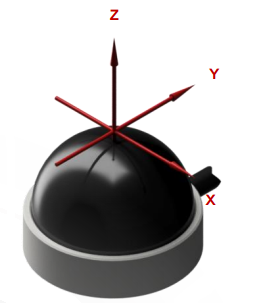
\includegraphics[scale=0.8]{Figures/OptoforceAxis3}
	\caption{Figure showing the x,y and z-direction for the 3d optical force used in this thesis \cite{OptoforceSheet}.}
	\label{fig:OptoforceAxis}
\end{figure}

\section{Robot} \label{sec:robot}
A Quadruped robot developed at the University of Oslo is shown in figure \ref{fig:robot}. The legs are about 45 cm long and mounted with optical force sensors. Four different gait is made by evolutionary algorithm and is developed by Nygaard et al. \cite{7850167}. The algorithm provides five types of gaits which is of either single-objective or multi-objective. 


\begin{figure}[h]
	\centering
	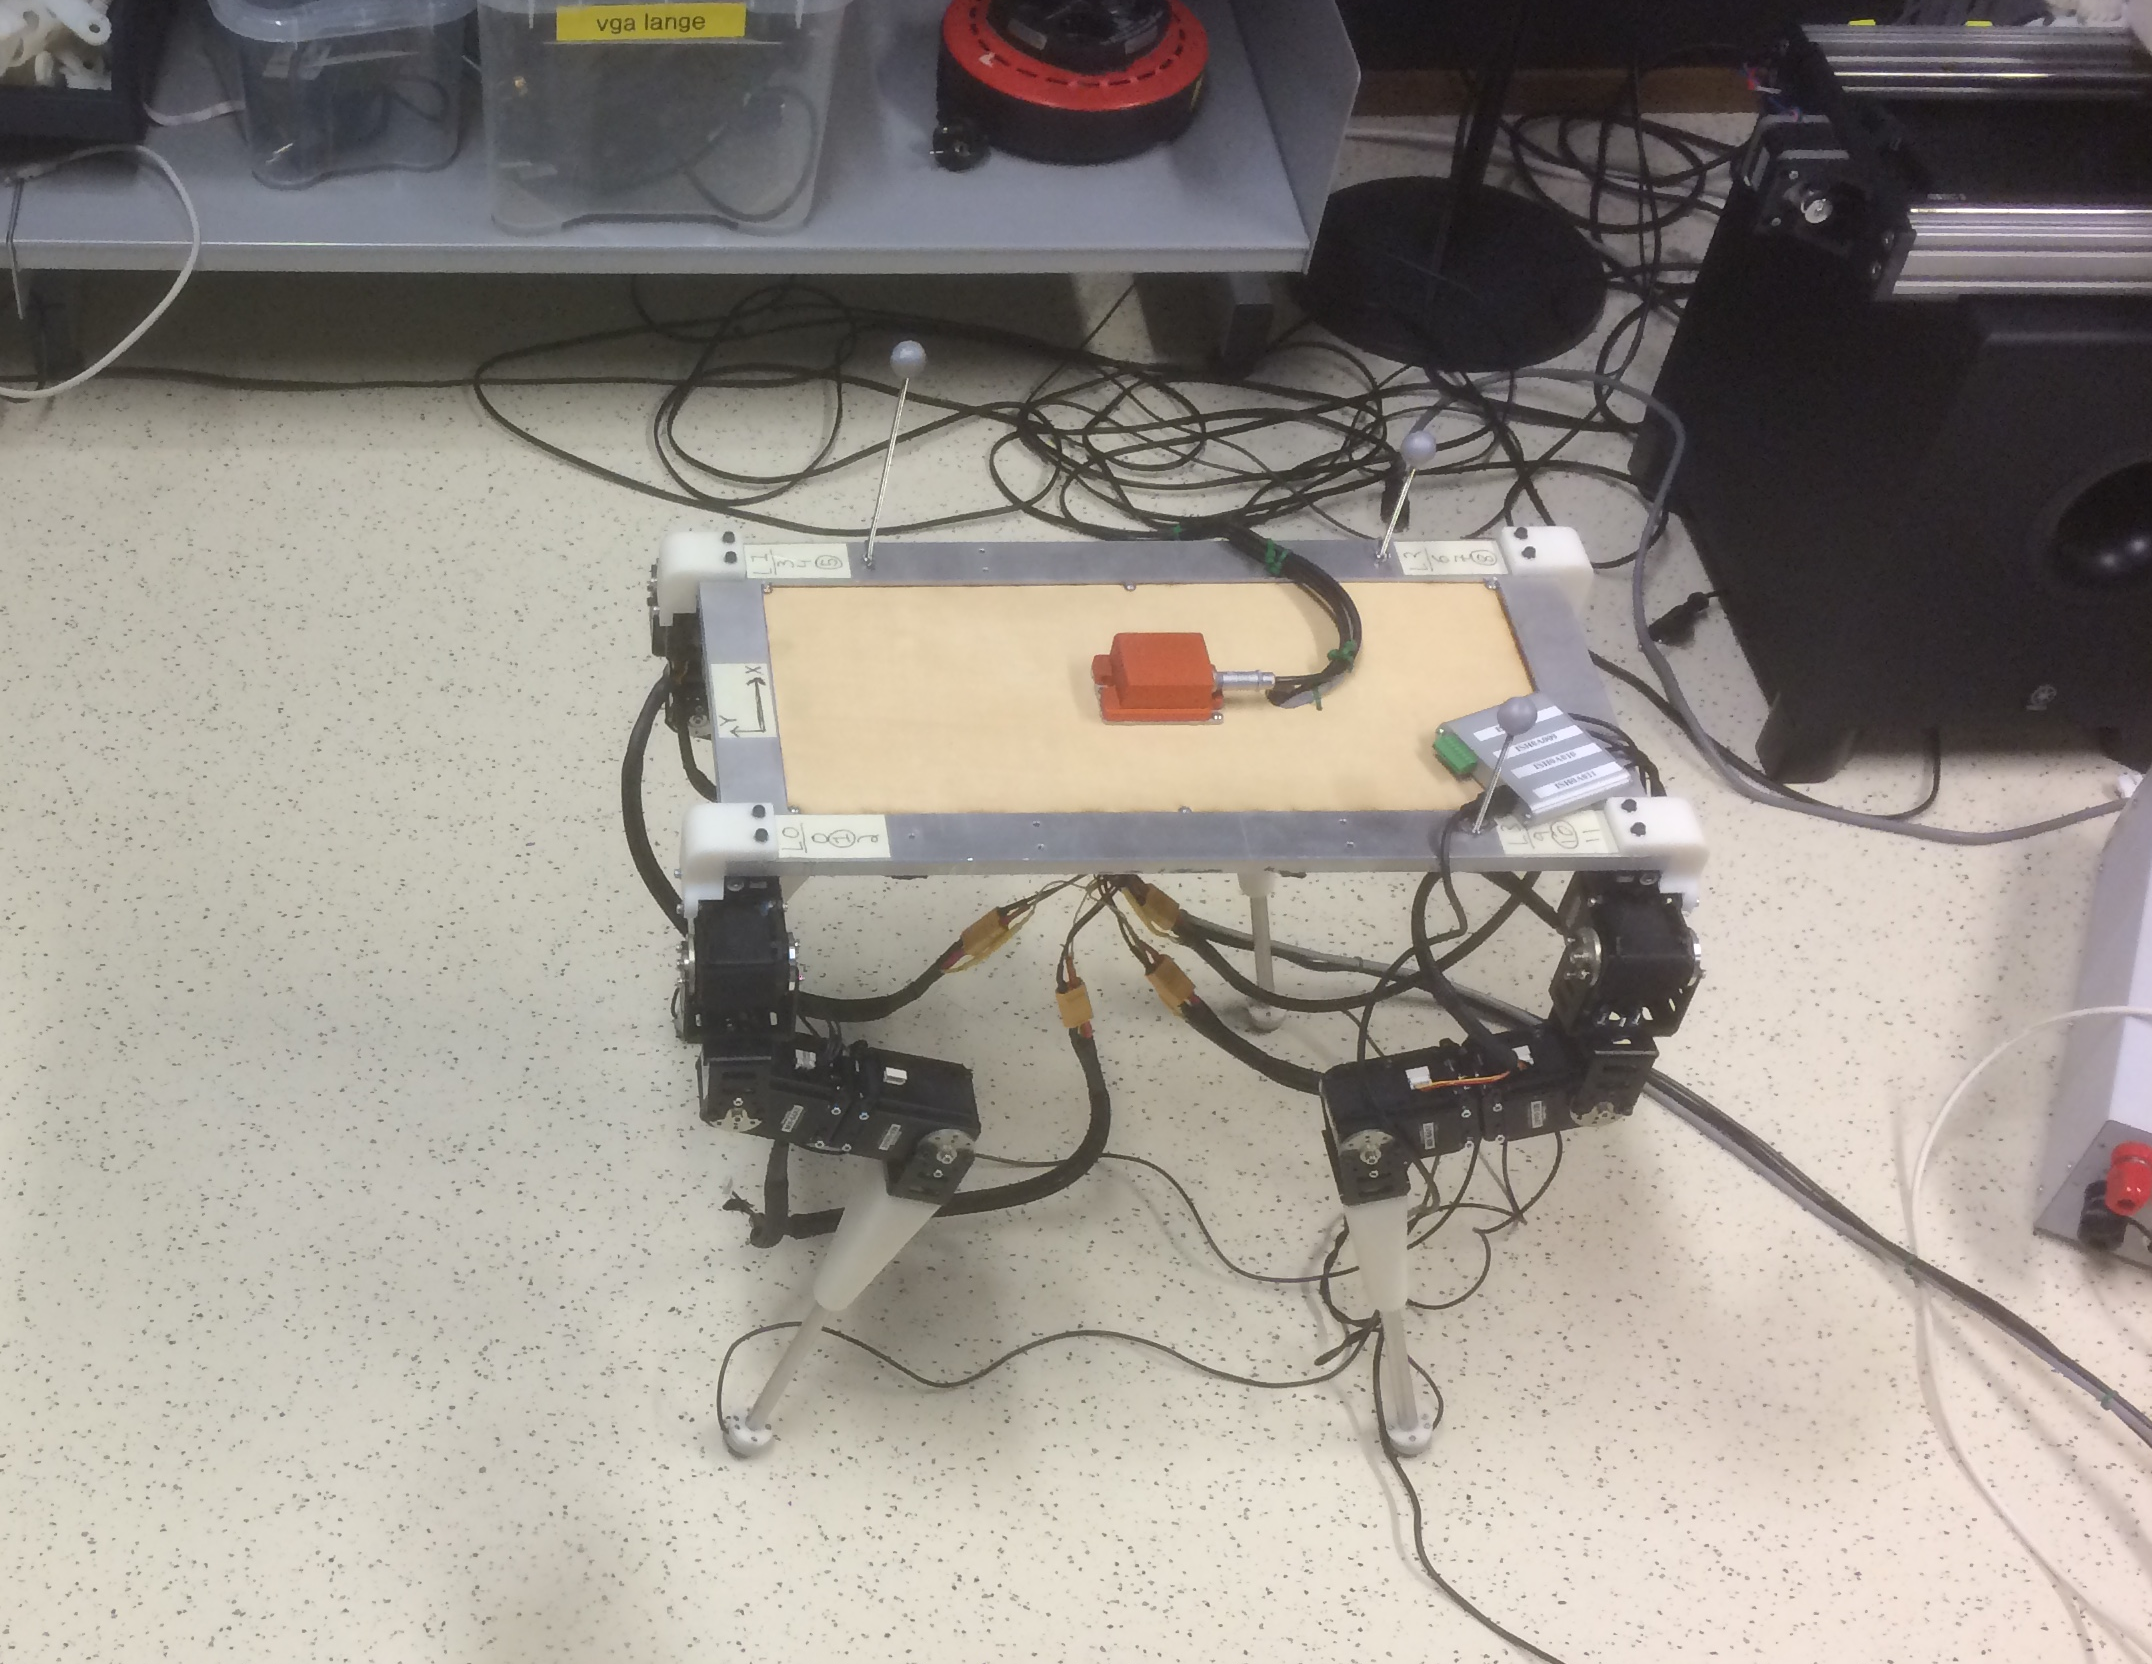
\includegraphics[width=\textwidth,height=\textheight,keepaspectratio]{Figures/Robot3}
	\caption{Figure showing the Quadruped Robot developed at the University of Oslo, which was used in all experiments}
	\label{fig:robot}
\end{figure}
\FloatBarrier


\section{Robot operating system}
The robot mentioned in section \ref{sec:robot}, operates on a Robot operating system (ROS) \cite{ROSintro}. ROS is an open source software framework and used to create robot applications. ROS consists of nodes that can be grouped into packages and be shared and distributed. A node is a process that perform computation. For instance a node could be controlling the robot, while the other one control prediction of terrain. This allow parallel execution of the data collection and class prediction in real time. Currently, the most compatible programming language are Python, C++, and Lisp.

\subsection{Messages and topics}
A message is a data structure which could be integer, floating point, arrays etc. Nodes can use the message to send out a message by publishing it a given topic \cite{ROSconcept}. The topic is used to identify the content of the message where a node has the possibility to subscribe to the appropriate topic. This can be seen as many-to-many one-way transport.

\subsection{Services}
When a many-to-many one-way communication is not appropriate, service and client provide a request and reply interaction \cite{ROSconcept}. A service can be either requesting or replying to the client. The client calls the service by sending the request message and awaiting the reply.


\subsection{Bag}
Rosbag is a package for recording and playing back ROS message data \cite{ROSconcept}. This has the benefit of storing sensor data which is necessary for developing and testing algorithms.


\subsection{ROS driver for the Optoforce sensor}  
A ROS driver for optical force sensor is from \cite{optoRos}. The node is able to read data from the sensor with 100Hz and will publish the data stream as floats to a topic. 


\section{Algorithms libraries}
Python provide lots of libraries which reduce developing time. The libraries are well-documented and have the freedom to customize each algorithm to use.

\paragraph{Scikit-learn}
Scikit-learn \cite{scikit-learn} is an open source library that provide tools for data mining and data analysis. The library is dependent on numpy, scipy and matplotlib. All of classifiers, and preprocessing data tool can be found in this library. 

\paragraph{Runstats}
Runstats \cite{runstats} is used to compute statistics, such as max, mean, skew, variance and standard deviation where some of them is described in section \ref{sub:statical}.


\chapter{Implementation}\label{ch:implementation}        %% ... or ??
This chapter intends to explain the various choices which has been made to create machine learning models.

\section{Environment setup}	
Four different terrains are used in the experiments: floor, carpet, soft mat, and hard mat as shown in figure \ref{fig:terrains}. A reason for choosing these is to get a more challenging task for classifier to distinguish them, because of similar properties. The intuition is that if the algorithm manages to discriminate between floor and carpet, it should be able to distinguish other terrains as well. Floor, carpet and hard mat has the most similar properties, and is also the most difficult to distinguish. They are all slippery, and has nearly equally hardness. Soft mat differ from the other with its softness and high friction. The experiments will be investigating whether the classifier can distinguish these terrains with minor differences.
\\
\\
The quadruped robot and the mounted optical force sensor used in this thesis are mentioned in chapter \ref{chap:software}. Only one gait is used in this project, which is a balanced multi-objective gait which let the robot have a straight locomotion. The reason is that the other gaits had issues when walking on the soft mat. The robot either got stuck with slow gait, or fell with fast gait. 

\begin{figure*}[h]
	\centering
	\begin{subfigure}[b]{0.475\textwidth}
		\centering
		\includegraphics[width=\textwidth]{Figures/Gulv2}
		\caption[Floor]%
		{{\small Floor}}    
		\label{fig:mean and std of net14}
	\end{subfigure}
	\hfill
	\begin{subfigure}[b]{0.475\textwidth}  
		\centering 
		\includegraphics[width=\textwidth]{Figures/Teppe2}
		\caption[]%
		{{\small Carpet}}    
		\label{fig:mean and std of net24}
	\end{subfigure}
	\vskip\baselineskip
	\begin{subfigure}[b]{0.475\textwidth}   
		\centering 
		\includegraphics[width=\textwidth]{Figures/MykMatte2}
		\caption[]%
		{{\small Soft mat}}    
		\label{fig:mean and std of net34}
	\end{subfigure}
	\quad
	\begin{subfigure}[b]{0.475\textwidth}   
		\centering 
		\includegraphics[width=\textwidth]{Figures/Hardmatte2}
		\caption[]%
		{{\small Hard mat}}    
		\label{fig:mean and std of net44}
	\end{subfigure}
	\caption[ ]
	{\small Four different terrain used for classification} 
	\label{fig:terrains}
\end{figure*}
\FloatBarrier

\section{Choice of implementation language}
Since the robot operating on ROS, and ROS is currently compatible with C++, Python or Lisp. Segmentation of data, described later in section \ref{subseq:segmentation}, is implemented in C++, due to fast computation. However, C++ does not provide many learning libraries, hence the learning algorithm is implemented in Python. 
			
\section{Data from optical force sensor}
This section will first describe how the measurement from sensor gathered. Next, it will present how the data is segmented into sequences and used as the basis for creating feature vectors.
	
\subsection{Data collection}
Data was gathered by having the robot walking 10 steps on each terrain. The runs were recorded into rosbag, which makes it possible to re-simulate the runs. Five runs for each terrain, and in total 20 runs were recorded. This gives in total 200 steps on each terrain for one sensor, and 800 steps with all four sensors together. However, in this thesis, only data from left front foot of the robot is used.
	
\subsection{Analyzing data from sensor}\label{sec:analyzopto}
Analyzing the data is to find common characteristics, and be able to segment desired data. Sensor data arrives in a stream as shown in figure \ref{fig:gtmgraf}. The periodic sequences is for each step. A common characteristic for all terrain is when the foot is in the air, it gives a minor change, almost constant, in x,y, z-direction. This characteristic will be used to segment desired data described in next section \ref{subseq:segmentation}. 


\begin{figure}[h]
	\centering
	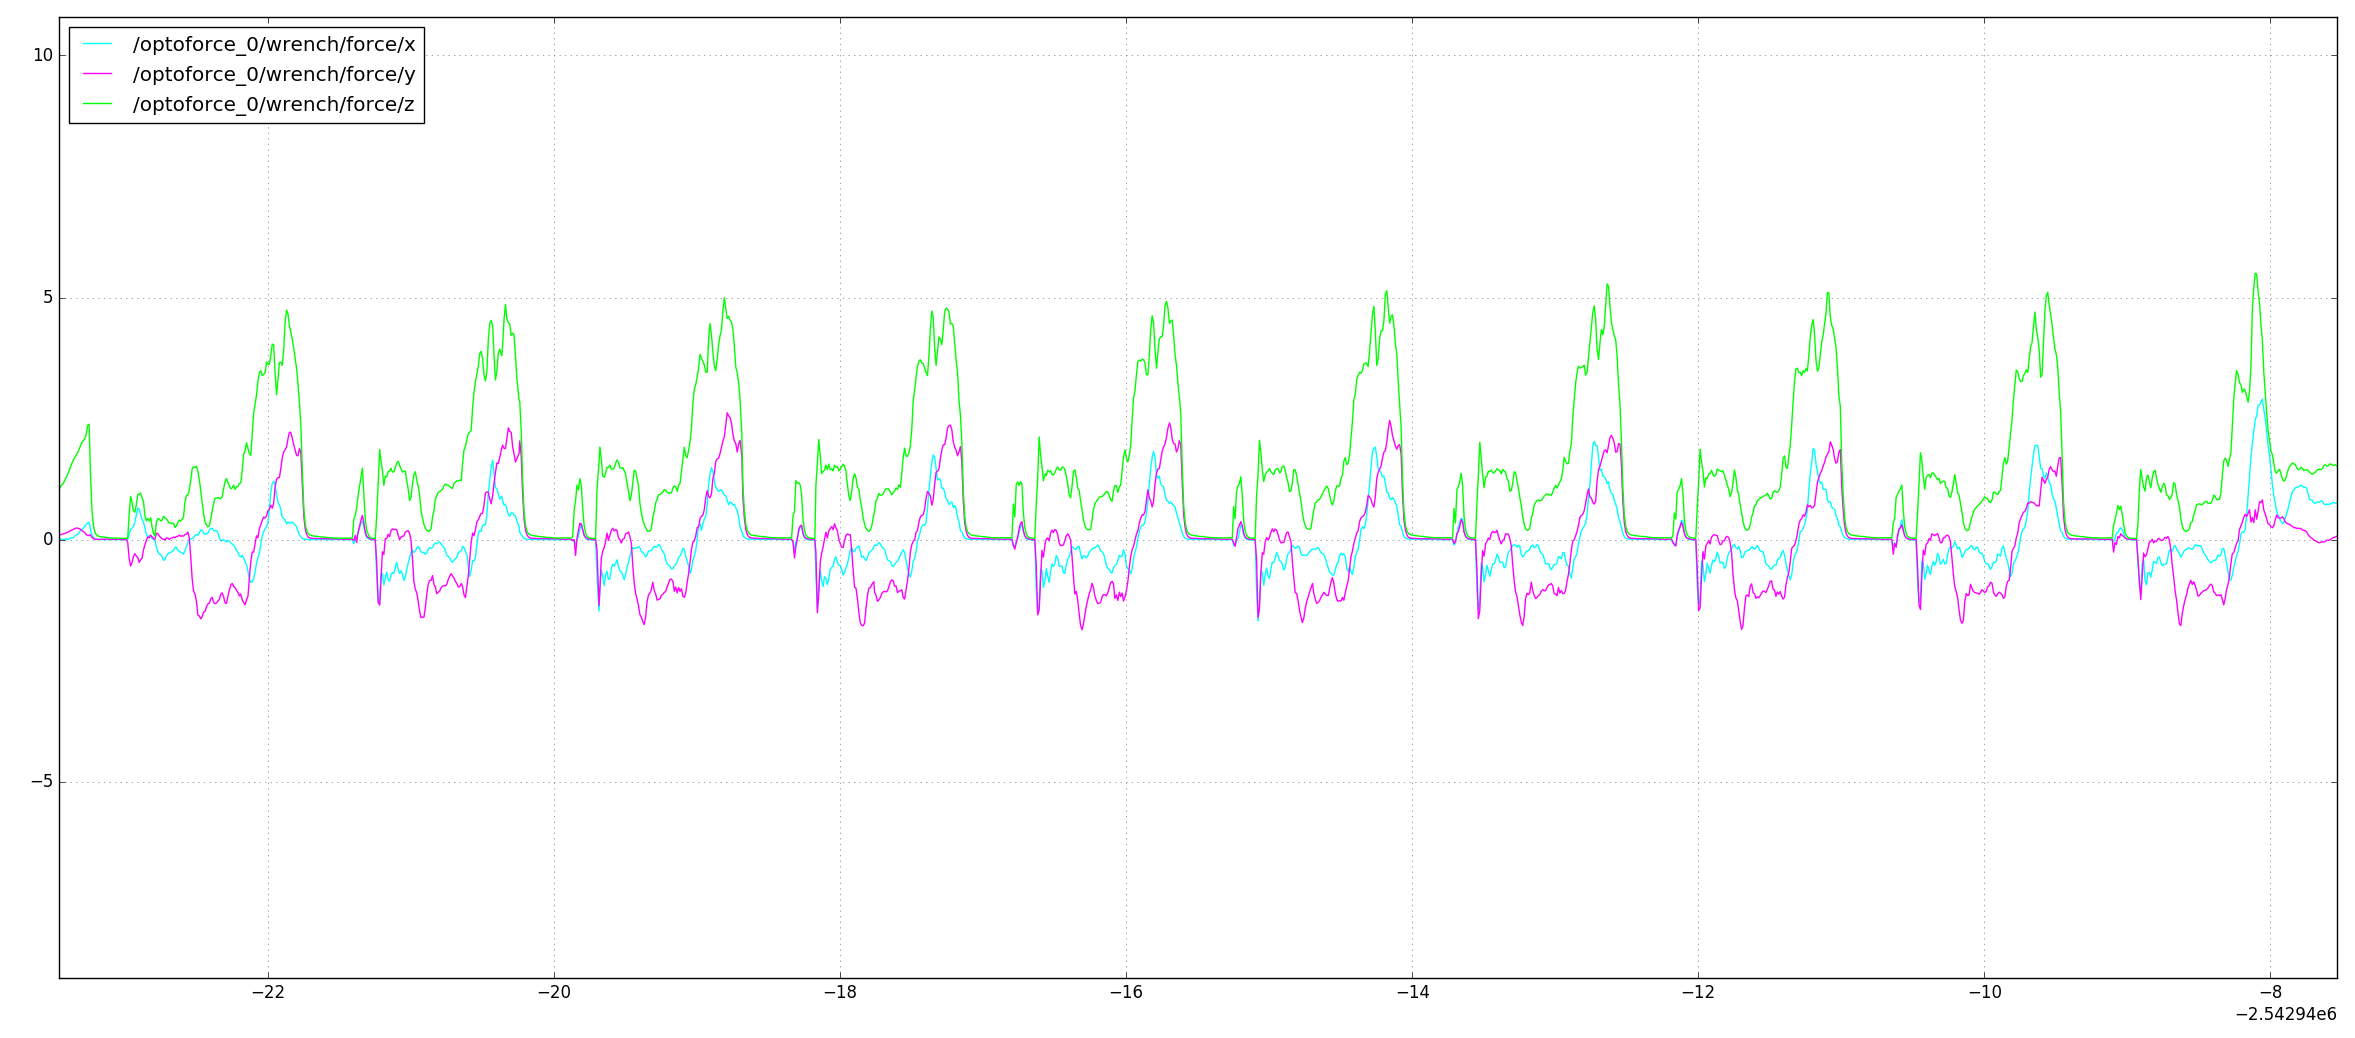
\includegraphics[width=\textwidth,height=\textheight,keepaspectratio]{Figures/gulvgraf}
	\captionsetup{labelformat=empty}
	\caption{(a) Floor}
	\label{fig:gulvgraf}
\end{figure}

\begin{figure}[h]
	\centering
	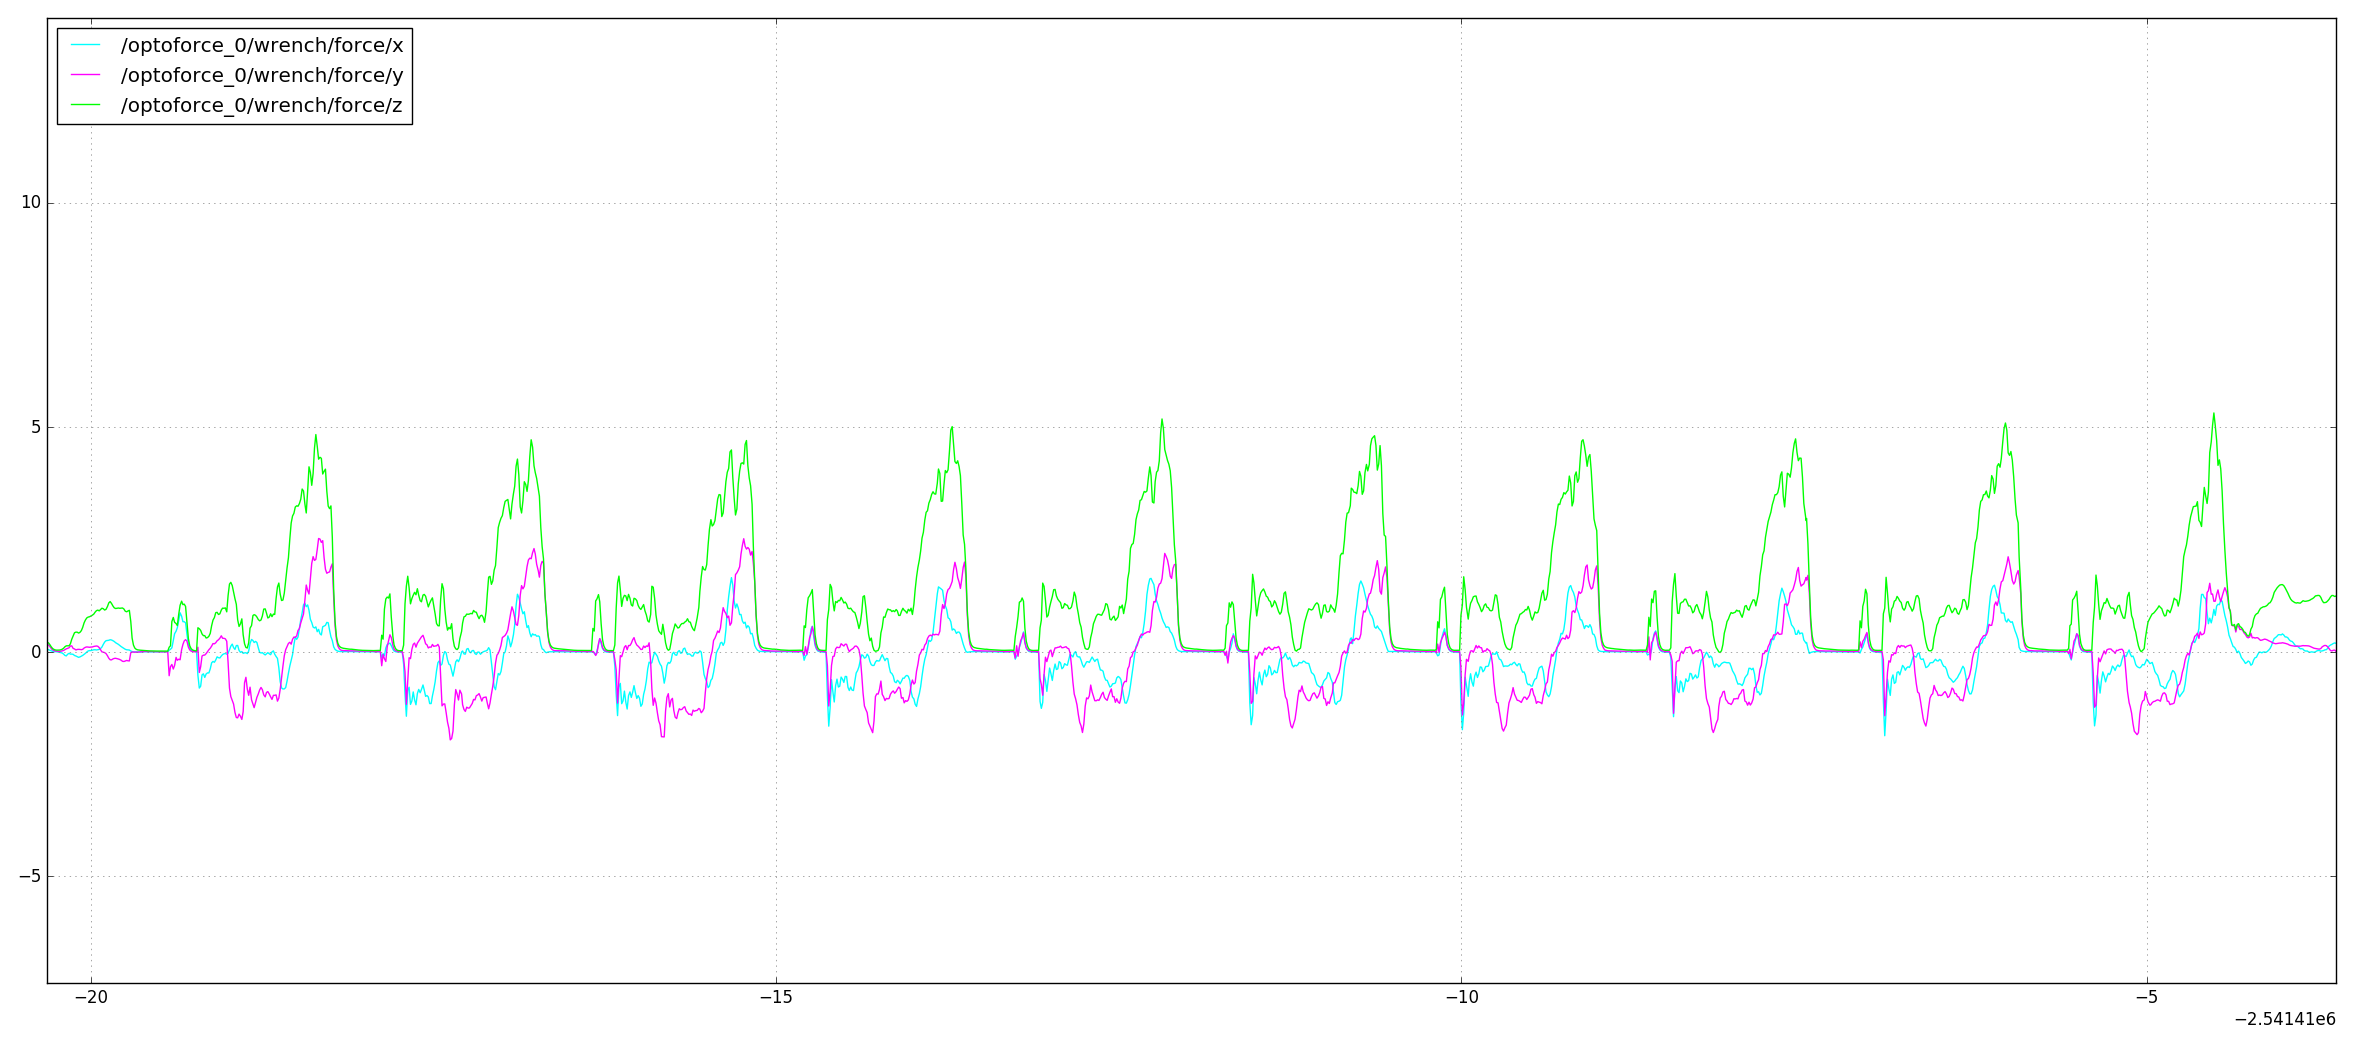
\includegraphics[width=\textwidth,height=\textheight,keepaspectratio]{Figures/teppegraf}
	\captionsetup{labelformat=empty}
	\caption{(b) Carpet}
	\label{fig:teppegraf}
\end{figure}

\begin{figure}[h]
	\centering
	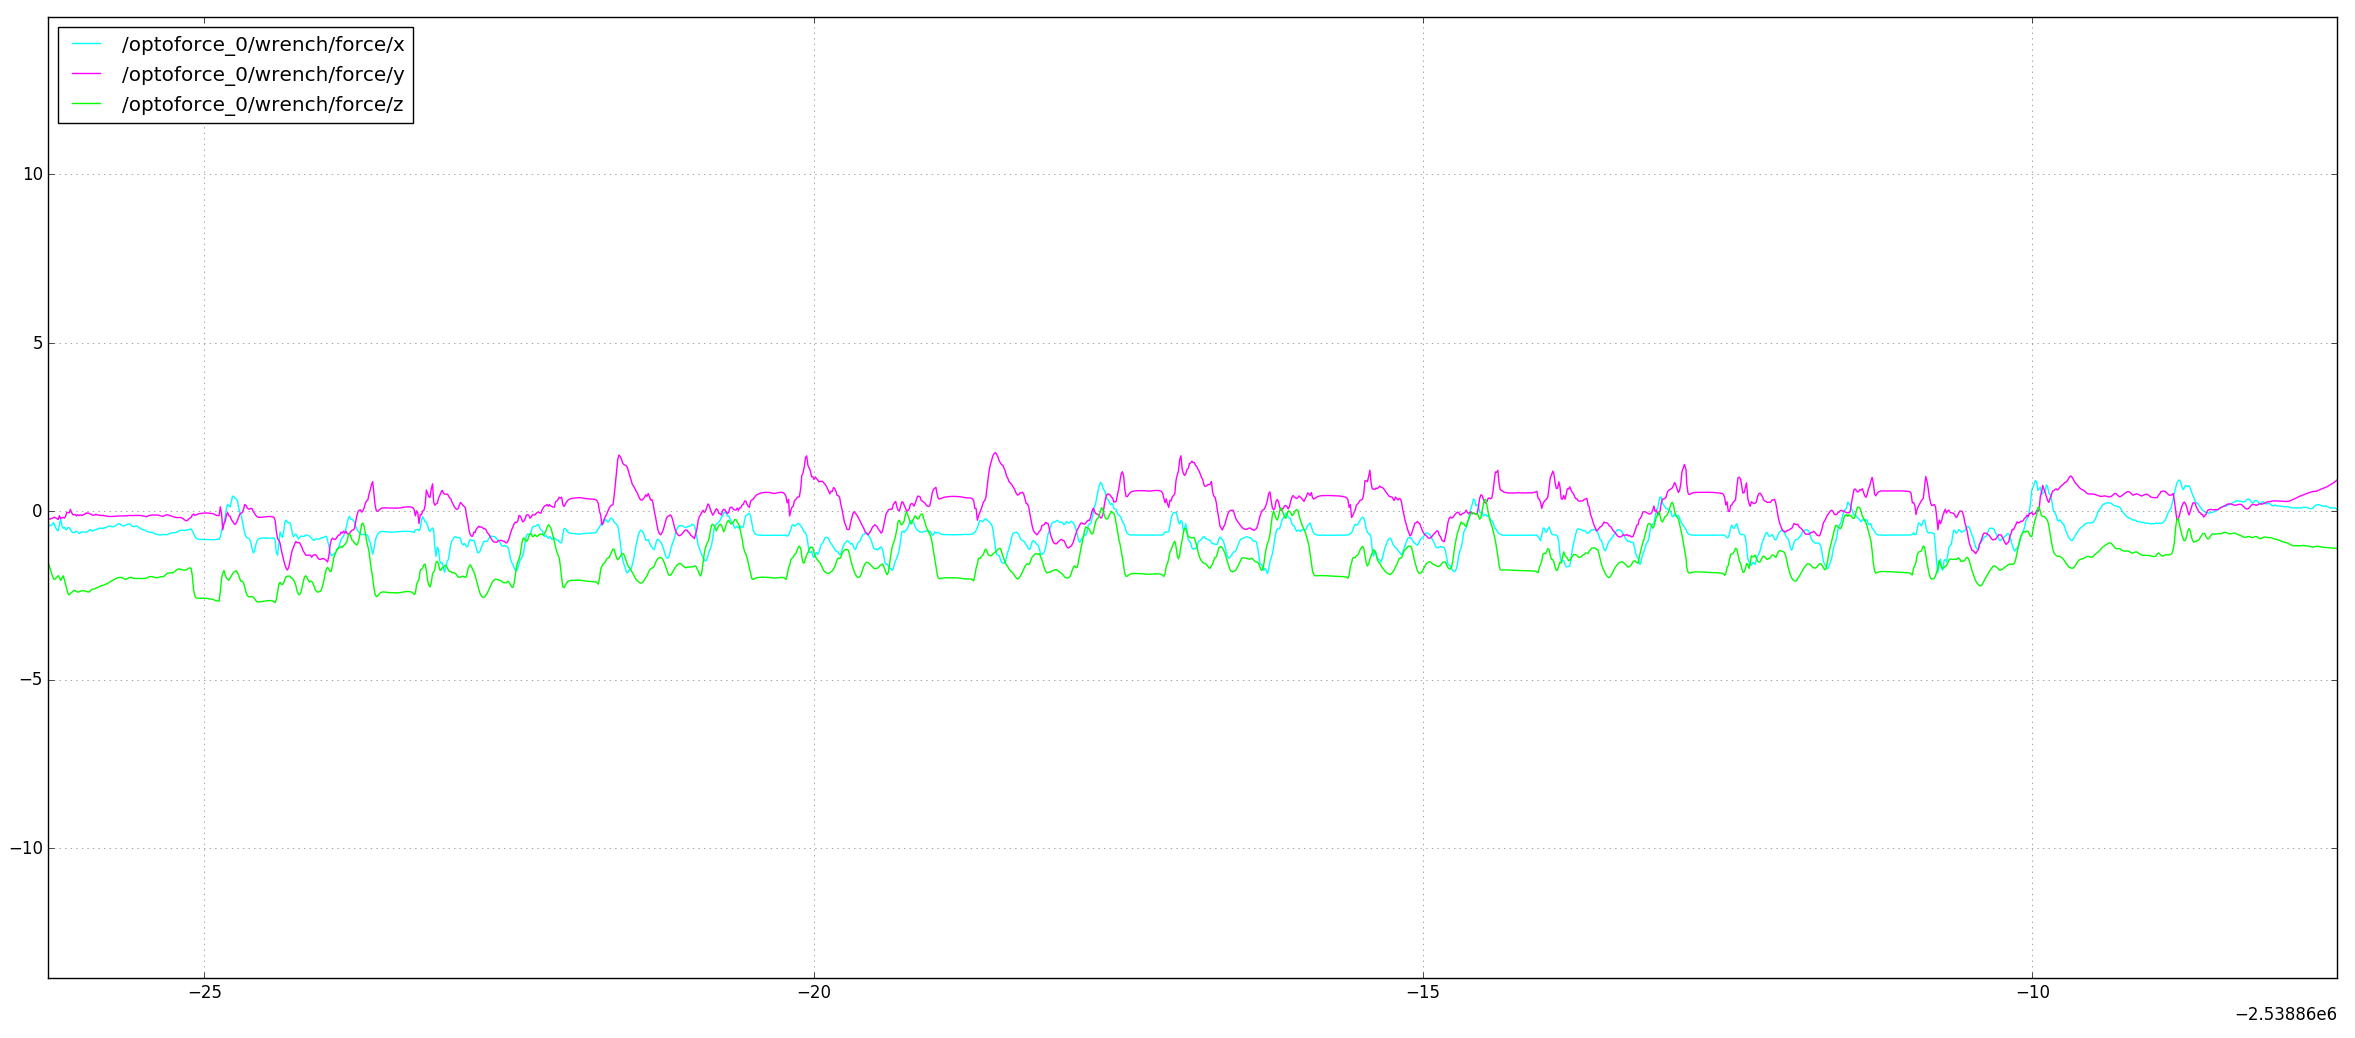
\includegraphics[width=\textwidth,height=\textheight,keepaspectratio]{Figures/mykmattegraf}
	\captionsetup{labelformat=empty}
	\caption{(c) Soft mat}
	\label{fig:mykmattegraf}
\end{figure}

\setcounter{figure}{0}
\begin{figure}[h]
	\centering
	\begin{subfigure}[t]{\textwidth}
		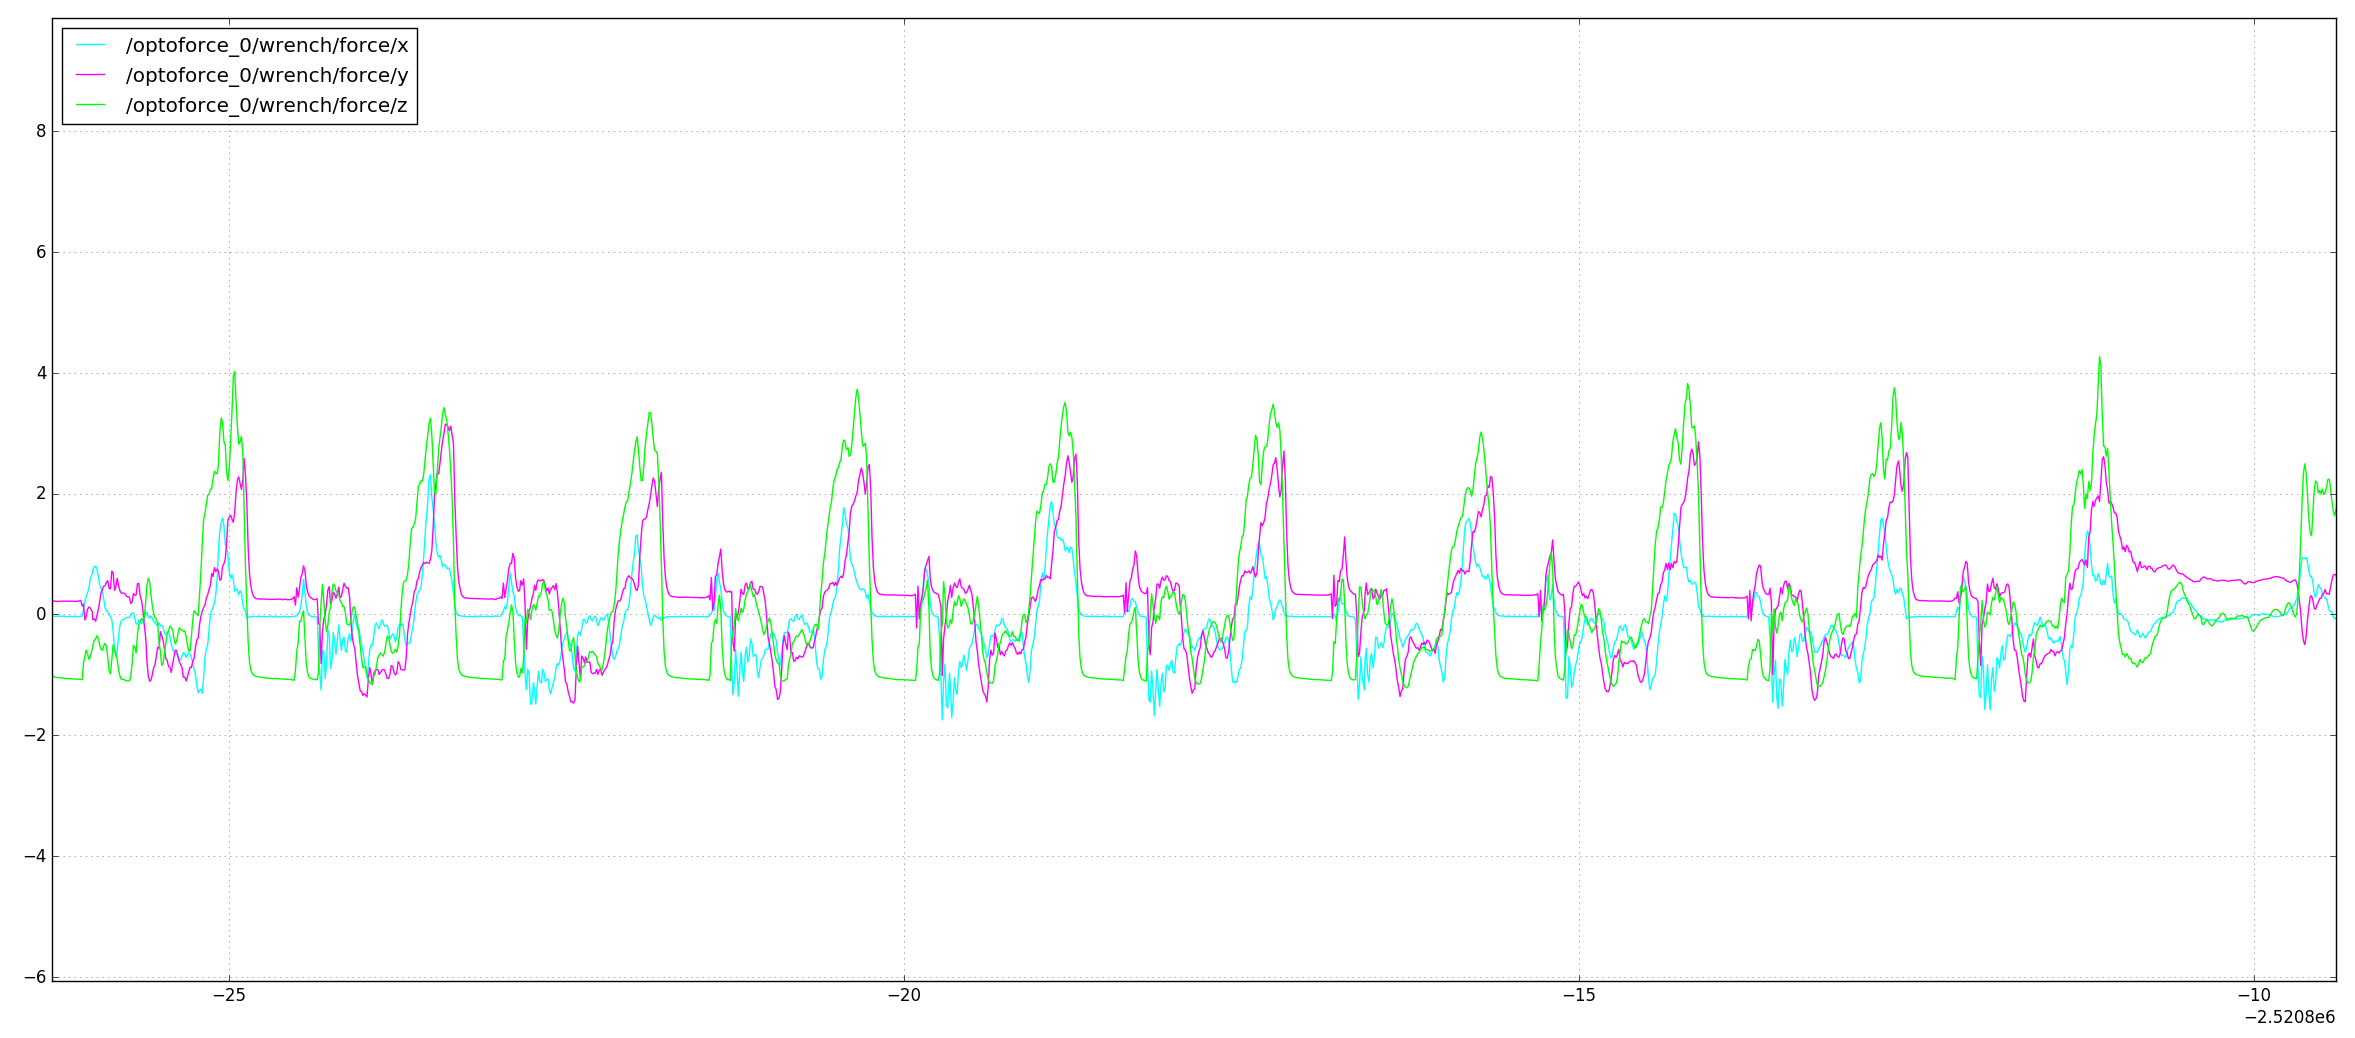
\includegraphics[width=\textwidth,height=\textheight,keepaspectratio]{Figures/mattebgraf}
		\captionsetup{labelformat=empty}
		\caption{(d) Hard mat}
		\label{fig:mattebgraf} 
	\end{subfigure}
	\caption{Figure showing an example data stream for each terrain. (a) floor (b) carpet (c) hard mat (d) soft mat.}
	\label{fig:gtmgraf}
\end{figure}
\FloatBarrier

\subsection{Data segmentation} \label{subseq:segmentation}
An appropriate method to segment data is by sliding window algorithm, however, difficulty to decide an acceptable size of the window, difficulty of determining whether the data is relevant from the window, and too big window size is not efficient. Thus, a custom algorithm to segment data was created. 
\\
\\
In the thesis, it is considered that the most informative data of terrain is from when the foot is on the ground. The custom algorithm will be storing the data sequences when the foot is on the ground, and stops when it is not on the ground. As mentioned in section \ref{sec:analyzopto}, a characteristic for all terrain when a foot is in the air, is that the x, y, and z-direction to a sensor has minor change in their values within a short sequence. Using this property gives the possibility to determine when a foot is either in air or on ground. In the implementation, two thresholds have to be sets; one for consider the minor change in each direction, one for consider minimum length of the minor change sequence, and they are set to 0.009 and 15 respectively. That is, when the data sequence consists at least 15 elements, and the difference between the currently data and its neighbor do not exceed 0.009, it is considered that the foot is in the air. When a foot reach the ground, there will be a big change in each direction for the sensor, and the program will start to store the data from sensor into an array until it is in the air again. Each step will be used as a sample in training and test set. The source code of segmenting desired data for one sensor can be found in appendix \ref{ap:code}.

\section{Feature sets}\label{sec:featuresets}
As mentioned in section \ref{features}, a good classifier is dependent of good features. As mostly of previous work have been extracting features both in time domain and frequency domain, this thesis will also be extracting in both domains. Five different feature set will be created and used to learn and evaluate each of classifiers. The following paragraphs will be introducing each sets.

\paragraph{Feature set one - raw data} 
This feature set use all data from each step in x, y and z-direction. As the length vary, the feature vector is decimated in front and end of the sequence to achieve a fixed length, in this case 125.  Choices of the sequence length and method of decimating is described in next section \ref{subseq:FixLength}. The feature vector set will look like:
	

\begin{align}\label{eq:f1}
f_{set1} &= \left\{ x_1,\dotsc,x_{125}, \right.\nonumber\\
&\qquad \left. {} y_1, \dotsc,y_{125}, \right.\nonumber\\
&\qquad \left. {} z_1,\dotsc,z_{125} \right\}
\end{align}


The vector contain 125 features from each 3 directions, which is in total 375 features.
	

		
		
	
\paragraph{Feature set two - statistical features} 
This feature set extracts statistical features from the dataset. As mentioned in section \ref{sub:relatedfeatures}, much of early work has been extracting the features with statistical metrics. Thus, this thesis will be using similar features. Calculation of some statistical metrics are described in section \ref{sub:statical}. The features created in this set will be from each direction, x,y and z in time domain: 
	
	%This is using some of the features from this article \cite{Hoffmann20141790}. 
	
	\begin{enumerate}
		\item The maximum value of the dataset in time domain
		\item The minimum value of the dataset in time domain
		\item The mean of the dataset in time domain
		\item The variance of the data set in time domain
		\item Skew in time domain
		\item Kurtosis in time domain 
		\item Standard deviation in time domain
	\end{enumerate}
	
The feature set will be look like:
	
\begin{align}
	f_{set2} &= \left\{ x_{max},x_{min},x_{skew},x_{kuortosis},x_{std},x_{var},x_{mean}, \right.\nonumber\\
	&\qquad \left. {} y_{max},y_{min},y_{skew},y_{kuortosis},y_{std},y_{var},y_{mean}, \right.\nonumber\\
	&\qquad \left. {} z_{max},z_{min},z_{skew},z_{kuortosis},z_{std},z_{var},z_{mean} \right\}
\end{align}
The vector contains 7 features from each direction, which is in total 21 features. 
	
\paragraph{Feature set three - complete frequency spectrum} 
Previous work has shown that using frequency has given good results. In this feature set, the raw data from time domain is transformed into the frequency domain by fast Fourier transform. After transformation, a decimation is used to achieve a fixed length. Since the minimum of length in time domain is 125, and the fast Fourier transform is symmetric, the minimum length of entire spectrum will be 62.5, however in this approach will be decimating to a length of 61. Contrary to decimate in front and end of the sequence, it is considered that data at end of the sequence is less important than in front, hence, these features will be discarded.
	
\begin{align}\label{eq:f1}
f_{set3} &= \left\{ fx_1,\dotsc,fx_{61}, \right.\nonumber\\
&\qquad \left. {} fy_1, \dotsc,fy_{61}, \right.\nonumber\\
&\qquad \left. {} fz_1,\dotsc,fz_{61}\right\}
\end{align}

The vector contains 61 features from each direction, which is in total 183 features. 
	
\paragraph{Feature set four - statistical features} 
This feature set compute the statistical metrics similar to feature set two, but in frequency domain. Additionally the energy of the spectrum suggested in \cite{26b23e912c654fe4b7478fd910130195}, by calculating the sum of the squares of the amplitudes is also used.
	
\begin{enumerate}
		\item The maximum value of the dataset in frequency domain
		\item The minimum value of the dataset in frequency domain
		\item The mean of the dataset in frequency domain
		\item The variance of the data set in frequency domain
		\item Skew in frequency domain
		\item Kurtosis in frequency domain 
		\item Standard deviation in frequency domain
		\item Energy 
\end{enumerate}
The feature vector which will be fed into the classifier:
\begin{align}
	f_{set3} &= \left\{ fx_{max},fx_{min},fx_{skew},fx_{kuortosis},fx_{std},fx_{var},fx_{mean},fx_{E}, \right.\nonumber\\
	&\qquad \left. {} fy_{max},fy_{min},fy_{skew},fy_{kuortosis},fy_{std},fy_{var},fy_{mean}fy_{E}, \right.\nonumber\\
	&\qquad \left. {} fz_{max},fz_{min},fz_{skew},fz_{kuortosis},fz_{std},fz_{var},fz_{mean},fz_{E} \right\}
	\end{align}
The vector contains 8 features from each direction, which is in total 24 features. 
	
\paragraph{Feature set five - set two and four} 
Good features might come from different feature sets. This set will collect feature set two and four into one unified set:
	\begin{align}
	f_{set5} &= \left\{ x_{max},x_{min},x_{skew},x_{kuortosis},x_{std},x_{var},x_{mean}, \right.\nonumber\\
	&\qquad \left. {}   y_{max},y_{min},y_{skew},y_{kuortosis},y_{std},y_{var},y_{mean}, \right.\nonumber\\
	&\qquad \left. {}  z_{max},z_{min},z_{skew},z_{kuortosis},z_{std},z_{var},z_{mean}, \right.\nonumber\\
	&\qquad \left. {} fx_{max},fx_{min},fx_{skew},fx_{kuortosis},fx_{std},fx_{var},fx_{mean},fx_{E}, \right.\nonumber\\
	&\qquad \left. {} fy_{max},fy_{min},fy_{skew},fy_{kuortosis},fy_{std},fy_{var},fy_{mean}fy_{E}, \right.\nonumber\\
	&\qquad \left. {} fz_{max},fz_{min},fz_{skew},fz_{kuortosis},fz_{std},fz_{var},fz_{mean},fz_{E} \right\}
	\end{align}
	
The vector contains 15 features from each direction, which is in total 45 features. 
	
\subsection{Achieving a fixed length of the sequences} \label{subseq:FixLength}
In order to use raw data as input, a fixed length is required. After many runs the length of data sequence vary between 125 to 135. Thus, the steps will be decimated to a constant length of 125. A simplified method for achieving fixed length is in listing \ref{lst:fix_length}. Note the technique is simplified to one-dimensional array, while in thesis use a 3-dimensional array, but the intention is same. Contrary to discard the data either in front or end of the sequence, this technique will be discarding on both sides, to retain the data in middle, which is considered as more informative data.
	
\lstinputlisting[language=Python, caption={A simplified method to achieve a fixed length of data sequence},captionpos=b,label={lst:fix_length},frame=single,breaklines=true]{code/fix_length.py}
	

	
%\newpage
\section{Learning approach}
The procedure of learning approach is divided into two processes: collecting data samples into files and the learning process.
	
\subsection{Collecting samples}
The first process is to gather data for each terrain and will be stored into files. Those files will be collected into a single file, and used as training and test samples in the next process. The procedure is shown in figure \ref{fig:createsamples}.
	
\begin{figure}[h]
	\centering
	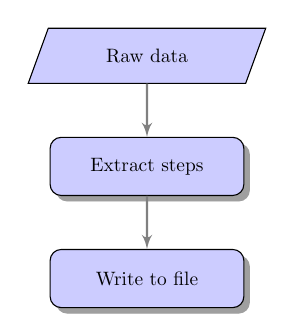
\begin{tikzpicture}[scale=0.7,transform shape]
		
	% Draw diagram elements
	\path \io{1}{Raw data};
		
	\path (p1.south)+(0,-1.5) \etape{2}{Extract steps};
	\path (p2.south)+(0.0,-1.5) \etape{3}{Write to file};
	

	%  \node [below=of p5] (p6-7) {};
	
	% Draw arrows between elements
	\path [line] (p1.south) -- node [above] {} (p2);
	\path [line] (p2.south) -- node [above] {} (p3);
	\end{tikzpicture}
	
	\caption{The figure showing process of creating a training file.} \label{fig:createsamples}
\end{figure}
	
\subsubsection{Procedure of creating samples} \label{sub:createsamples}
	\begin{enumerate}
		\item \textbf{\underline{Raw data}}
		\\
		The dataset is retrieved from the optical force sensor.
		
		\item \textbf{\underline{Extract steps}}
		\\
		Raw data will be partitioned into samples as described in section \ref{subseq:segmentation}.
		
		\item \textbf{\underline{Write to file}}
		\\
		This step will write each of data sequence into file with label of the terrain name.
		
		
\end{enumerate}
\clearpage

\subsection{Learning process} \label{subsec:learningProc}
When the data samples of each terrain is unified into a single file, the learning process is shown in figure \ref{fig:learningProcess}, is to evaluate each classifier. Rectangles are a processes that takes an given input and produces an output. The dashed rectangles are processes that can be omitted.
\begin{figure}[h]
	\centering
	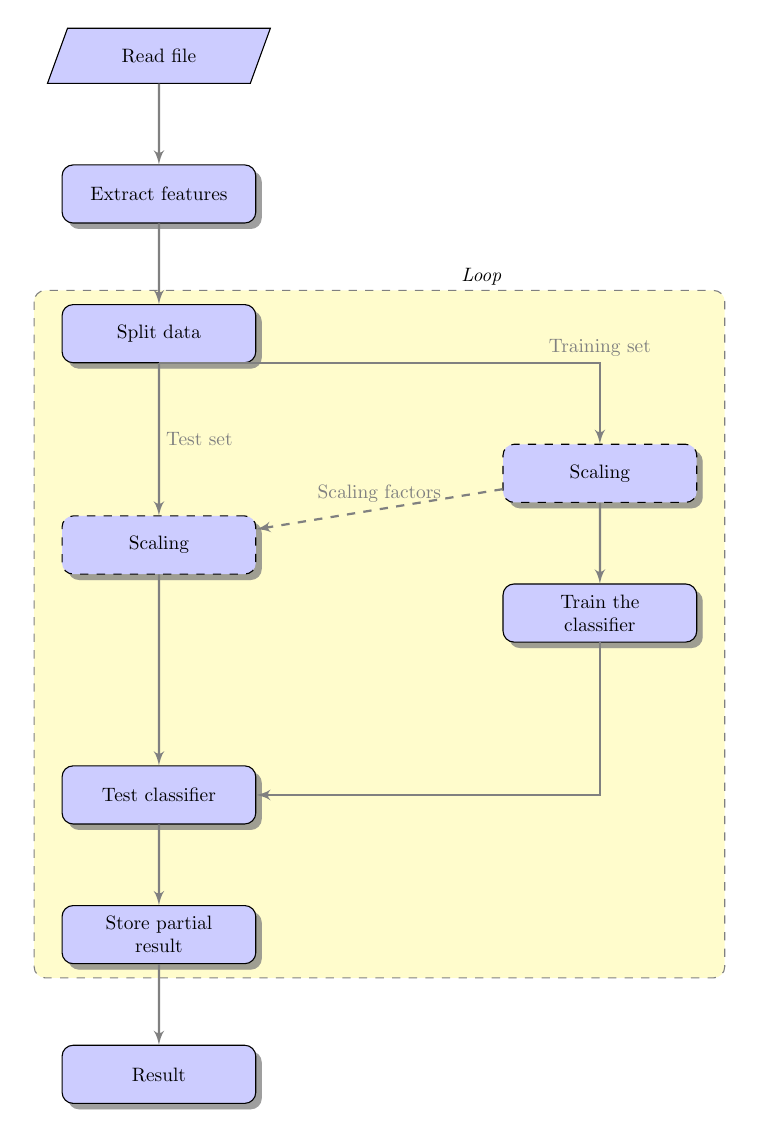
\begin{tikzpicture}[scale=0.7,transform shape]
	
	% Draw diagram elements
	%  \path \io{1}{Raw data};
	\path \io{2}{Read file};
	%  \path (p1.south)+(0,-1.5) \etape{2}{Extract steps};
	\path (p2.south)+(0.0,-2) \etape{3}{Extract features};	
	\path (p3.south)+(0.0,-2) \etape{4}{Split data};
	\path (p4.south)+(8,-2.0) \etapeTo{5}{Scaling};
	\path (p5.south)+(0,-2) \etape{6}{Train the classifier};
	\path (p4.south)+(0,-3.3) \etapeTo{9}{Scaling};
	\path (p9.south)+(0,-4.0) \etape{7}{Test classifier};		
	\path (p7.south)+(0,-2) \etape{10}{Store partial result};
	\path (p10.south)+(0,-2) \etape{8}{Result};
	
	%  \node [below=of p5] (p6-7) {};
	
	% Draw arrows between elements
	% \path [line] (p1.south) -- node [above] {} (p2);
	\path [line] (p2.south) -- node [above] {} (p3);
	\path [line] (p3.south) -- node [above] {} (p4);
	\path [line] (p4.south) -| node [above] {Training set} (p5);
	
	\path [line] (p5.south) -- node [above] {} (p6);
	\path [line] (p6.south) |- node [above] {} (p7);
	\path [line] (p4.south) -- node [right] {Test set} (p9);
	\path [line] (p7.south) -- node [above] {} (p10);
	\path [line] (p10.south) -- node [above] {} (p8);
	\path [line] (p9.south) -- node [above] {} (p7);
	%  \path [line] (p5.south) -- node [above] {Feature} (p9);
	\path [line,dashed] (p5) -- node [above]{Scaling factors} (p9);
	\background{p3}{p4}{p5}{p10}{Loop} 
	
	\end{tikzpicture}
	
	\caption{Figure showing process to evaluate a certain classifier.} \label{fig:learningProcess}
\end{figure}

\FloatBarrier
	\clearpage
\subsubsection{Details of the learning process} \label{sub:learningprocess}
\begin{enumerate}
\item \textbf{\underline{Reading file}}
\\
This step will take a file as input, created from section \ref{sub:createsamples}.
		
\item \textbf{\underline{Extract features}}
\\
This step will create one of the five feature sets as mentioned in section \ref{sec:featuresets}.
		
\item \textbf{\underline{Loop}}
		
\begin{enumerate} 
\item \textbf{\underline{Split data}} \label{en:loop}
\\
The extracted feature vectors is partitioned into a training and testing set. The cross validation is LOOCV, thus the training set consists of 199 samples and one test sample.
			
\item \textbf{\underline{Scaling}}
\\
This step takes the training set as input and standardize the data as mention in section \ref{subsec:scaling}. The scaling factor will used on the test data.
			
\item \textbf{\underline{Train the classifier}}
\\
The classifier will take the training set as input and train.
			
\item \textbf{\underline{Test classifier}} 
\\
This step use the model to predict the test set.

\item \textbf{\underline{Store partial result}} 
\\
This step will store the partial result of the test sample. If there are still more data to be predicted start from \ref{en:loop}.
\end{enumerate}	
		
\item \textbf{\underline{Result}}
\\
This step will compute the overall results as mentioned in section \ref{subsec:evalclf}, of performance to a certain chosen classifier. 
\end{enumerate}
	
\clearpage
\subsection{The evaluation}
To finding optimal feature combination and algorithm to the optical sensor, following steps will be investigated:

\begin{enumerate}
	\item Evaluate the performance of each five classifiers with different feature sets. Additionally, investigate whether a feature scaling is appropriate.  
	\item The learning process will be integrating with two different feature selection methods to achieve a better performance. 
	\item \label{it:data} Some of the top performer classifier along with the feature set will be further tested on new data samples.
	\item Selecting two best performer and use grid search with the training samples to find best parameters, and test on data samples collected in step \ref{it:data}.
	\item The best performed classifier will be used to evaluate the performance when the robot walks through two different terrains.
	\item Lastly, will test whether it is appropriate to use training sample from the one sensor to predict the other sensors. 
\end{enumerate}


\chapter{Experiments and results}                     %% ... or ??
The chapter presents results of all models in the previous chapter. This chapter is divided into 6 main sections, where each of them is the experiments. The first section will present the result of each classifier with the different sets of features. The second section will present a modified implementation to increase the performance. The third section will use top performed classifiers with its feature set to evaluated on new set of data samples. The fourth section will use a grid search to tune parameters to two top performed classifier, and compare to default values. The fifth section presents a real time implementation used to evaluate the performance of the best classifier when the robot walks on different terrains. Last section shows the possibility to use training samples from the one sensor to predict the other.
 
 
\section{Performance of each classifier}\label{result_exp1}
This section will present the results of each classifier along with an analysis.
	
\subsection{Results}
Table \ref{exp1} shows the result of each classifier when using the learning approach described in \ref{sub:learningprocess}. 
	
\begin{table}[h]
	\centering
	\resizebox{\textwidth}{!} & 83\% \\ \cmidrule(l){2-4} 
			\multicolumn{1}{l|}{} & \multicolumn{1}{l|}{Decision tree} & \multicolumn{1}{l|}{94\%} & 96\% \\ \cmidrule(l){2-4} 
			\multicolumn{1}{l|}{} & \multicolumn{1}{l|}{KNN} & \multicolumn{1}{l|}{89\%} & 91\% \\ \cmidrule(l){2-4} 
			\multicolumn{1}{l|}{} & \multicolumn{1}{l|}{Neural network} & \multicolumn{1}{l|}{95\%} & 96\% \\ \cmidrule(l){2-4} 
			\multicolumn{1}{l|}{} & \multicolumn{1}{l|}{SVM} & \multicolumn{1}{l|}{89\%} & 93\% \\ \midrule
			\multicolumn{1}{l|}{\multirow{5}{*}{\begin{tabular}[c]{@{}l@{}}Set two - \\ statistical features in \\ time domain\end{tabular}}} & \multicolumn{1}{l|}{Bayes Navies} & \multicolumn{1}{l|}{82\%} & 82\% \\ \cmidrule(l){2-4} 
			\multicolumn{1}{l|}{} & \multicolumn{1}{l|}{Decision tree} & \multicolumn{1}{l|}{83\%} & 84\% \\ \cmidrule(l){2-4} 
			\multicolumn{1}{l|}{} & \multicolumn{1}{l|}{KNN} & \multicolumn{1}{l|}{84\%} & 84\% \\ \cmidrule(l){2-4} 
			\multicolumn{1}{l|}{} & \multicolumn{1}{l|}{Neural network} & \multicolumn{1}{l|}{83\%} & 88\% \\ \cmidrule(l){2-4} 
			\multicolumn{1}{l|}{} & \multicolumn{1}{l|}{SVM} & \multicolumn{1}{l|}{76\%} & 85\% \\ \midrule
			\multicolumn{1}{l|}{\multirow{5}{*}{\begin{tabular}[c]{@{}l@{}}Set three - \\ complete frequency \\ domain\end{tabular}}} & \multicolumn{1}{l|}{Bayes Navies} & \multicolumn{1}{l|}{91\%} & 91\% \\ \cmidrule(l){2-4} 
			\multicolumn{1}{l|}{} & \multicolumn{1}{l|}{Decision tree} & \multicolumn{1}{l|}{83\%} & 82\% \\ \cmidrule(l){2-4} 
			\multicolumn{1}{l|}{} & \multicolumn{1}{l|}{KNN} & \multicolumn{1}{l|}{91\%} & 88\% \\ \cmidrule(l){2-4} 
			\multicolumn{1}{l|}{} & \multicolumn{1}{l|}{Neural network} & \multicolumn{1}{l|}{93\%} & 93\% \\ \cmidrule(l){2-4} 
			\multicolumn{1}{l|}{} & \multicolumn{1}{l|}{SVM} & \multicolumn{1}{l|}{52\%} & 93\% \\ \midrule
			\multicolumn{1}{l|}{\multirow{5}{*}{\begin{tabular}[c]{@{}l@{}}Set four - \\ statistical features in \\ frequency domain\end{tabular}}} & \multicolumn{1}{l|}{Bayes Navies} & \multicolumn{1}{l|}{81\%} & 81\% \\ \cmidrule(l){2-4} 
			\multicolumn{1}{l|}{} & \multicolumn{1}{l|}{Decision tree} & \multicolumn{1}{l|}{80\%} & 82\% \\ \cmidrule(l){2-4} 
			\multicolumn{1}{l|}{} & \multicolumn{1}{l|}{KNN} & \multicolumn{1}{l|}{88\%} & 84\% \\ \cmidrule(l){2-4} 
			\multicolumn{1}{l|}{} & \multicolumn{1}{l|}{Neural network} & \multicolumn{1}{l|}{85\%} & 88\% \\ \cmidrule(l){2-4} 
			\multicolumn{1}{l|}{} & \multicolumn{1}{l|}{SVM} & \multicolumn{1}{l|}{83\%} & 86\% \\ \midrule
			\multicolumn{1}{l|}{\multirow{5}{*}{\begin{tabular}[c]{@{}l@{}}Set five - \\ set 2,4\end{tabular}}} & \multicolumn{1}{l|}{Bayes Navies} & \multicolumn{1}{l|}{82\%} & 82\% \\ \cmidrule(l){2-4} 
			\multicolumn{1}{l|}{} & \multicolumn{1}{l|}{Decision tree} & \multicolumn{1}{l|}{79\%} & 80\% \\ \cmidrule(l){2-4} 
			\multicolumn{1}{l|}{} & \multicolumn{1}{l|}{KNN} & \multicolumn{1}{l|}{88\%} & 84\% \\ \cmidrule(l){2-4} 
			\multicolumn{1}{l|}{} & \multicolumn{1}{l|}{Neural network} & \multicolumn{1}{l|}{87\%} & 89\% \\ \cmidrule(l){2-4} 
			\multicolumn{1}{l|}{} & \multicolumn{1}{l|}{SVM} & \multicolumn{1}{l|}{83\%} & 86\% \\ \bottomrule
		\end{tabular}%
	}
	\caption{Table showing the result after following the approach shown in figure \ref{fig:learningProcess}}
	\label{exp1}
\end{table}
\FloatBarrier
	
	
\subsection{Analysis}
The result shown that all classifier have an accuracy of at least 70\%. Top performed classifiers are, Decision tree and Neural Network with an accuracy of 96\%. 
\\
\\
Regarding the feature scaling, SVM and KNN which use distances in their computation, only SVM had the biggest effect. KNN on other hand, was slightly affected by scaling, but mostly gave smaller accuracy. Neural Network achieved small improvement, while Decision tree either performed best with scaled or not scaled dependent on feature set, and Bayes Navies did not have any effect. Since the feature scaling achieved an big improvement with the SVM and minor on the other classifier, scaled features will be used in further experiments.
\\
\\
Among the highest results are either from whole raw data sequence or complete frequency domain. Regarding statistics features extracted in both domain, it shows a relative similar performance of for all of them. In the next experiment will therefore using all of the feature again. 
\\
\\
Beside of looking at the performance of each classifiers, it is also interesting to look how data provided from the sensor respond to different terrain. In time domain, which can be seen in figure \ref{fig:meanxyz}, the soft mat differ the most among the terrains. Forces from floor, carpet and hard mat in x-direction are relative similar as shown in figure \ref{fig:meanx}. Forces in y-direction as seen in figure \ref{fig:meany} are more distinguish, but still quite similar. While forces in z-direction as seen in figure \ref{fig:meanz}, distinguish each terrains even clearly. The carpet and hard mat provide similar forces, but the floor has most similar with the shapes of curves. In frequency domain, again, soft mat differ the most among the other. In contrast to similar data from floor, carpet and hard mat in time domain, in frequency domain the floor has a bigger differences from the other as seen in figure \ref{fig:meanxyz}. The carpet and hard mat on other hand are almost equally. However, it can be seen slightly difference between them in y, and z-direction shown in figures \ref{fig:ffty}, and \ref{fig:fftz} respectively.

\begin{figure} [h]
	\centering
	\begin{subfigure}[b]{0.95\textwidth}
		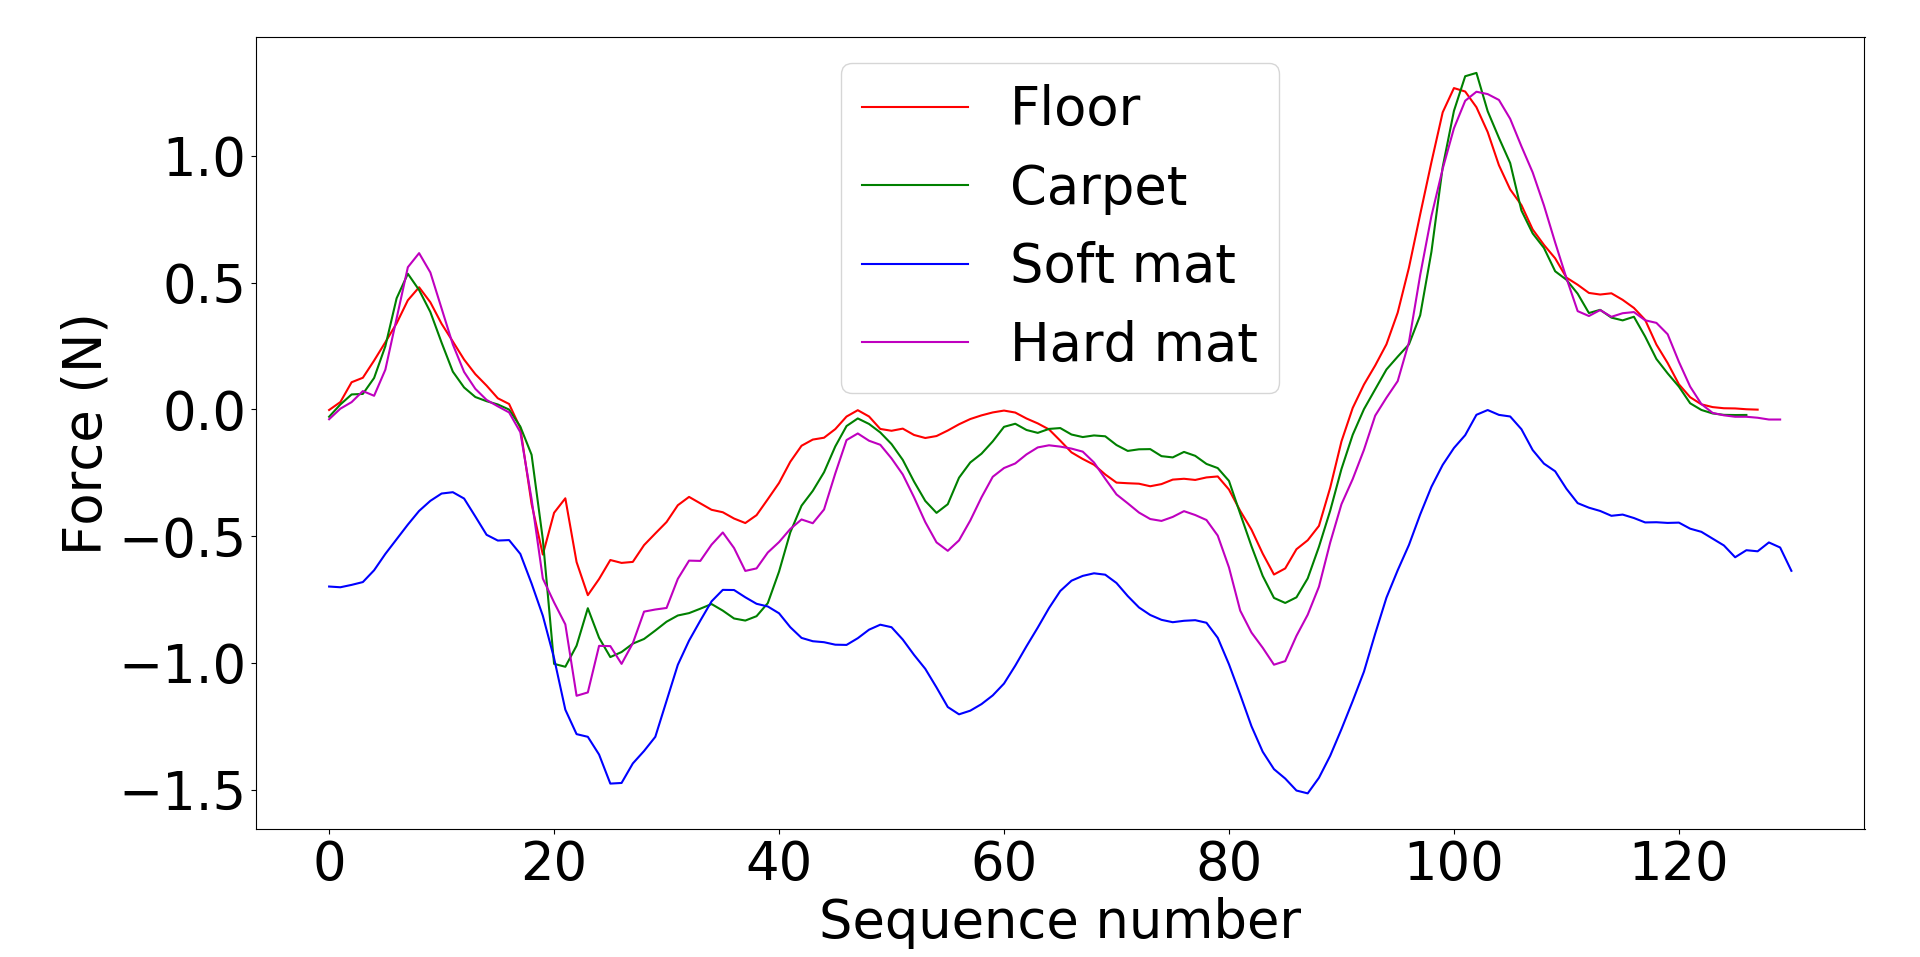
\includegraphics[width=\textwidth,height=\textheight,keepaspectratio]{Figures/x}
		\caption{Mean of 10 samples in x-direction}
		\label{fig:meanx} 
	\end{subfigure}
	
	\begin{subfigure}[b]{0.95\textwidth}
		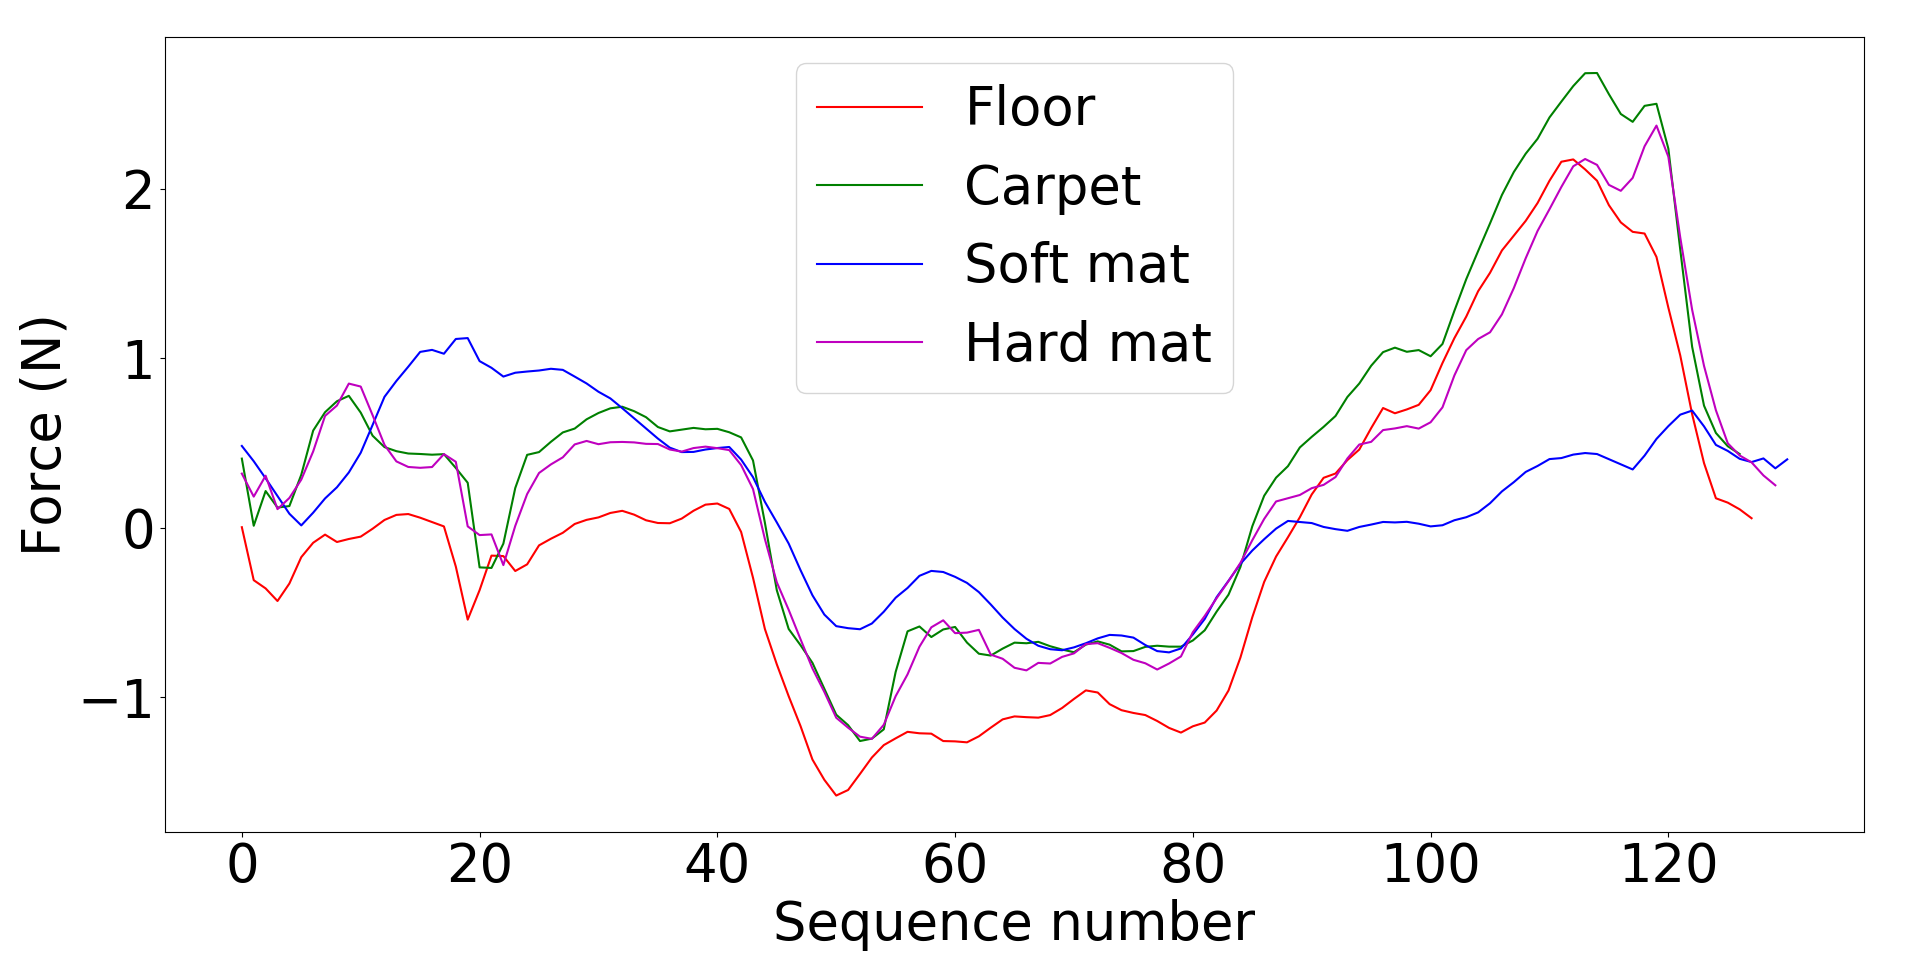
\includegraphics[width=\textwidth,height=\textheight,keepaspectratio]{Figures/y}
		\caption{Mean of 10 samples in y-direction}
		\label{fig:meany}
	\end{subfigure}
\end{figure}
\begin{figure}[h] \ContinuedFloat
	\begin{subfigure}[b]{0.95\textwidth}
		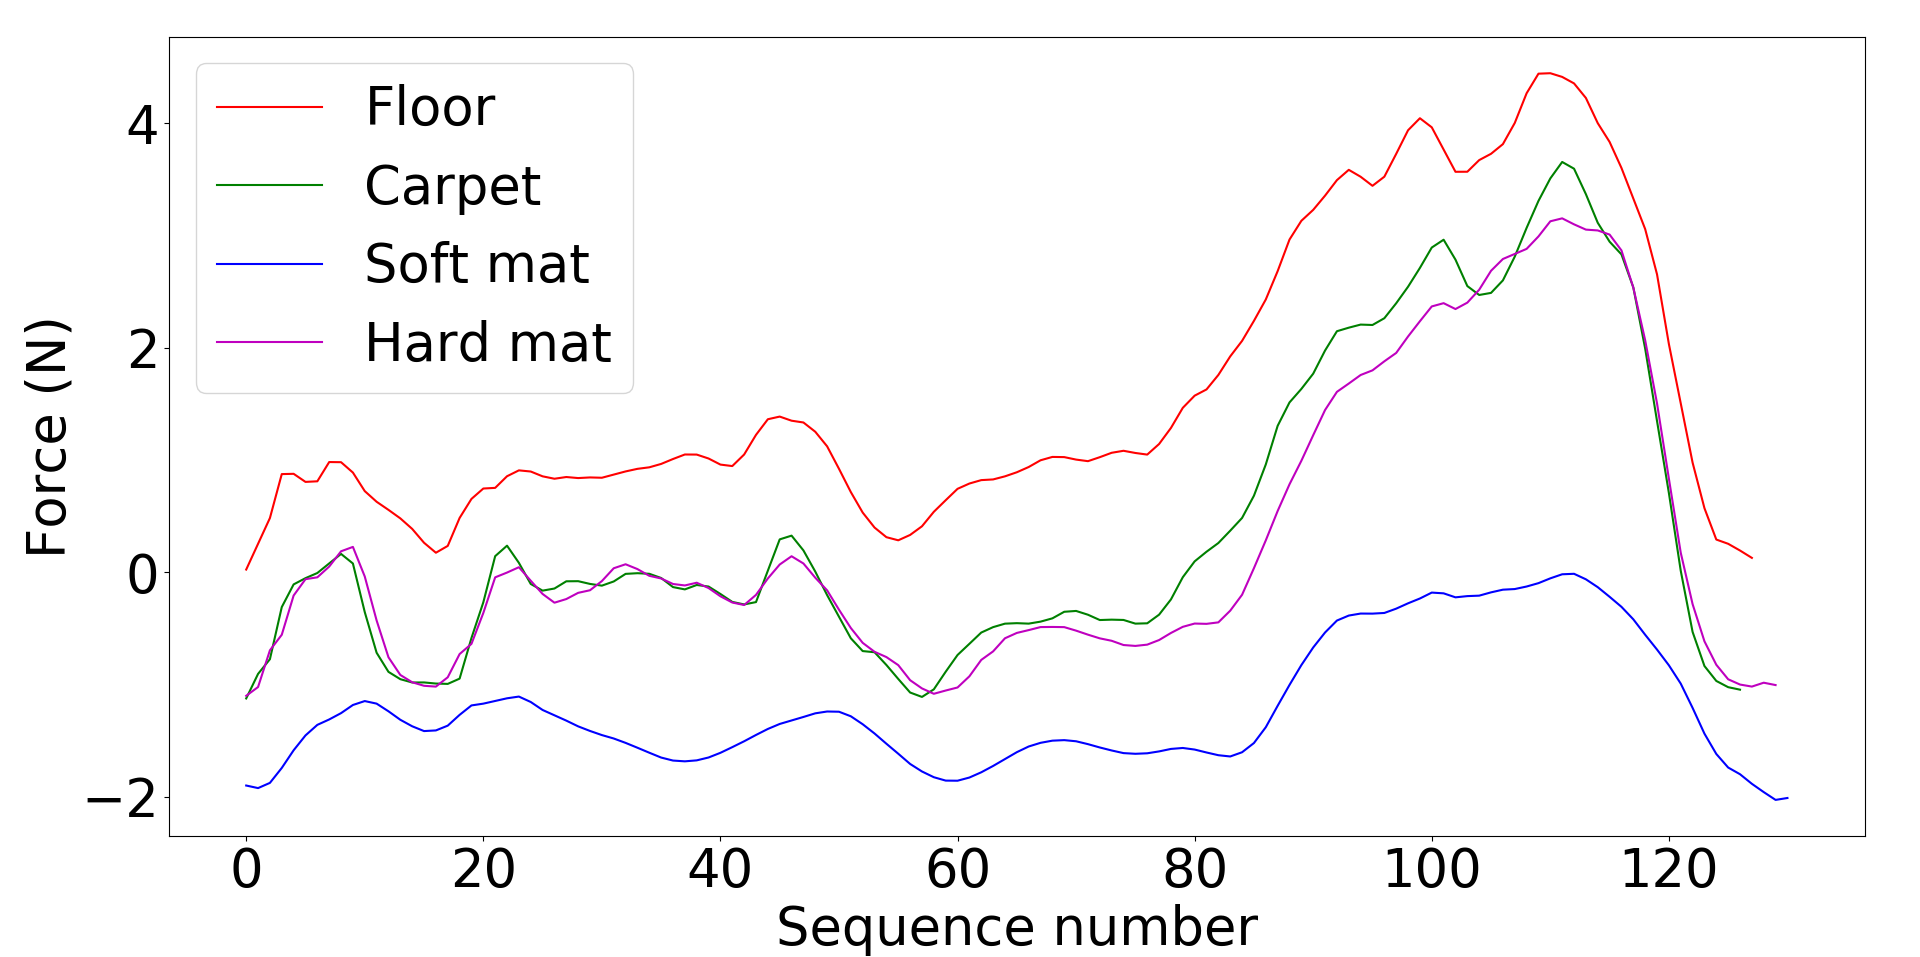
\includegraphics[width=\textwidth,height=\textheight,keepaspectratio]{Figures/z}
		\caption{Mean of 10 samples in z-direction}
		\label{fig:meanz}
	\end{subfigure}
	
	\caption[]{The figure showing the mean of 10 steps on each terrain different direction in time domain. (a) mean in the x-direction (b) mean in y-direction (c) in z-direction }
	\label{fig:meanxyz}
\end{figure}


\begin{figure}[h]
	\centering
	\begin{subfigure}[b]{0.95\textwidth}
		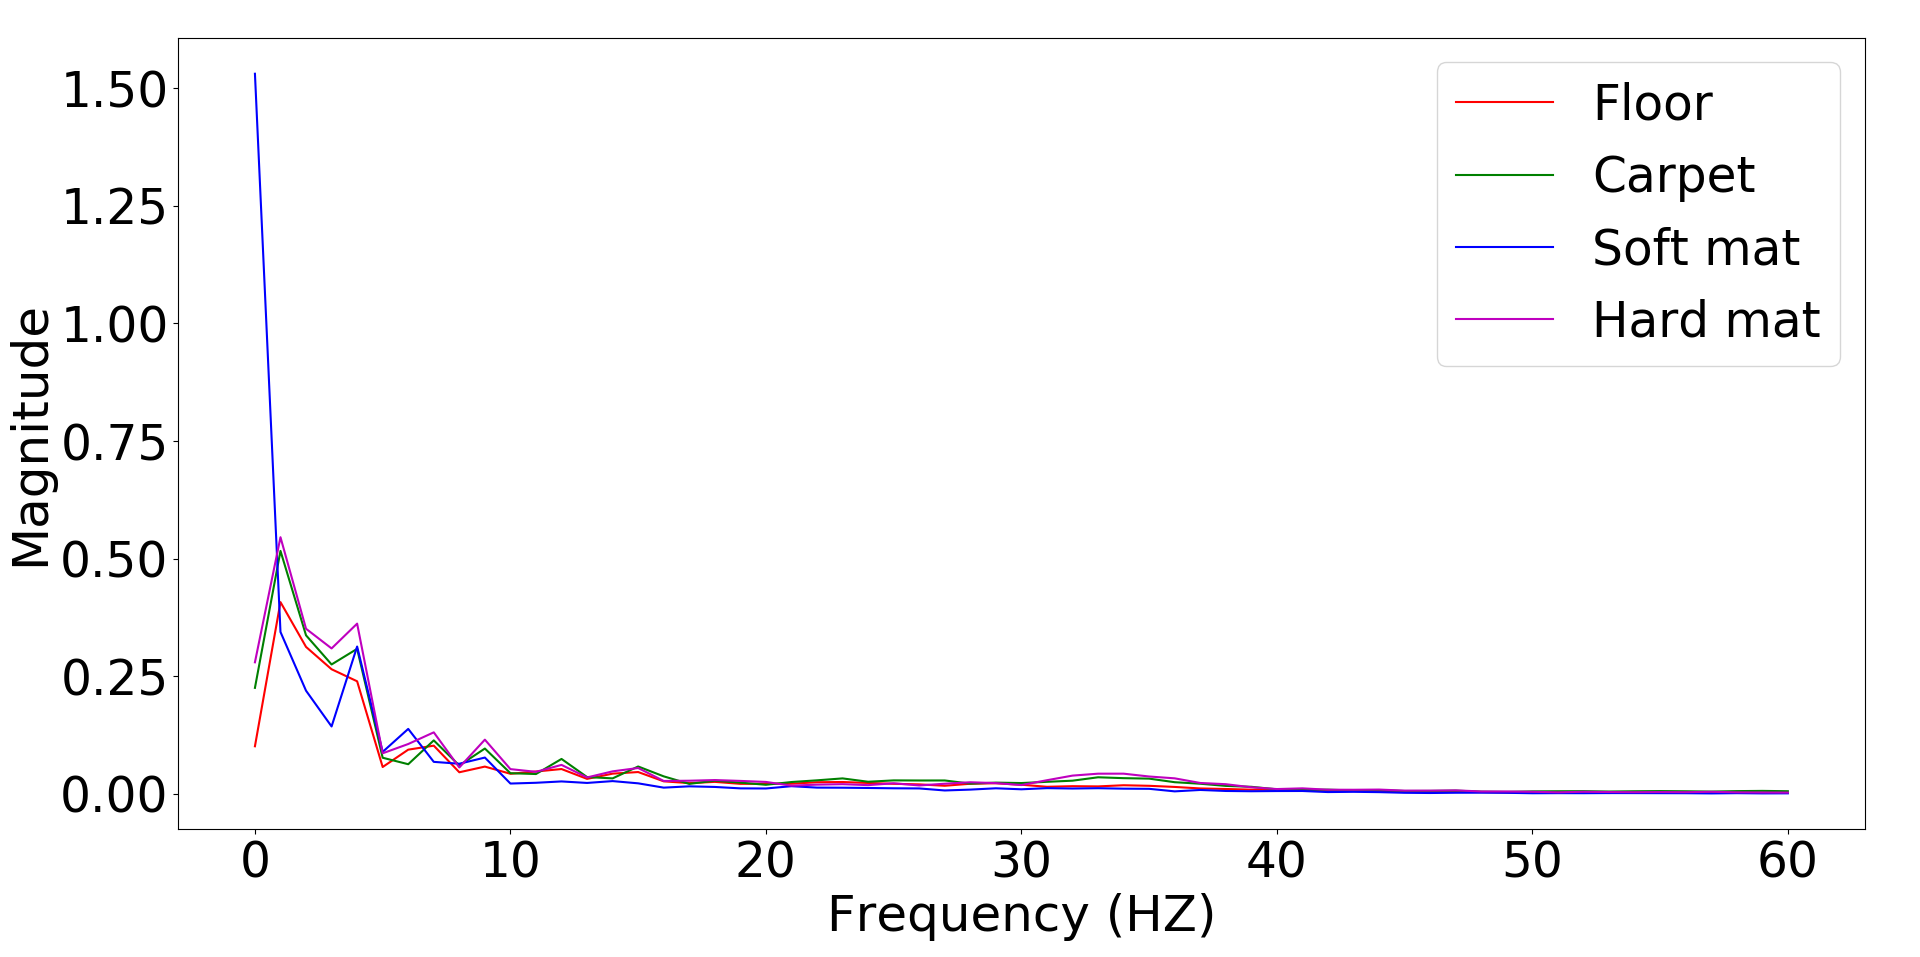
\includegraphics[width=1\linewidth]{Figures/fftx}
		\caption{Mean of 10 samples in x-direction}
		\label{fig:fftx} 
	\end{subfigure}
\end{figure}
\begin{figure}[h] \ContinuedFloat	
	\begin{subfigure}[b]{0.95\textwidth}
		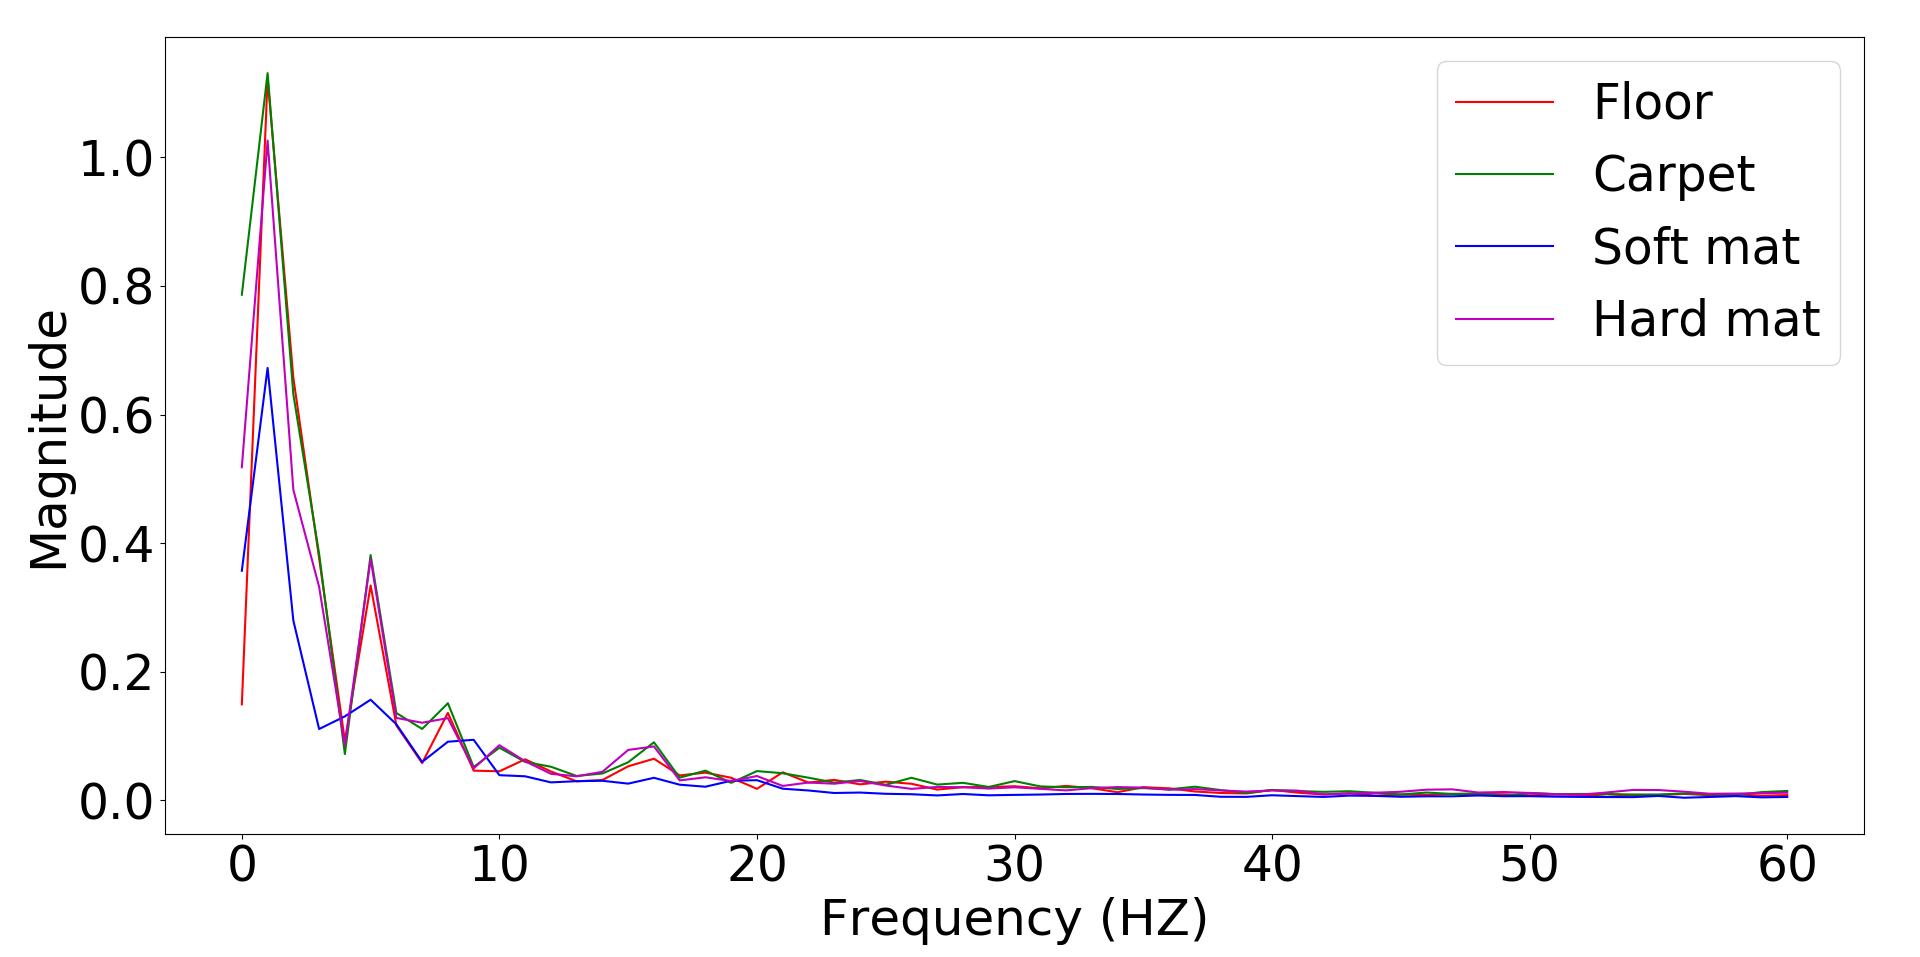
\includegraphics[width=1\linewidth]{Figures/ffty}
		\caption{Mean of 10 samples in y-direction}
		\label{fig:ffty}
	\end{subfigure}
	
	
	\begin{subfigure}[h]{0.95\textwidth}
		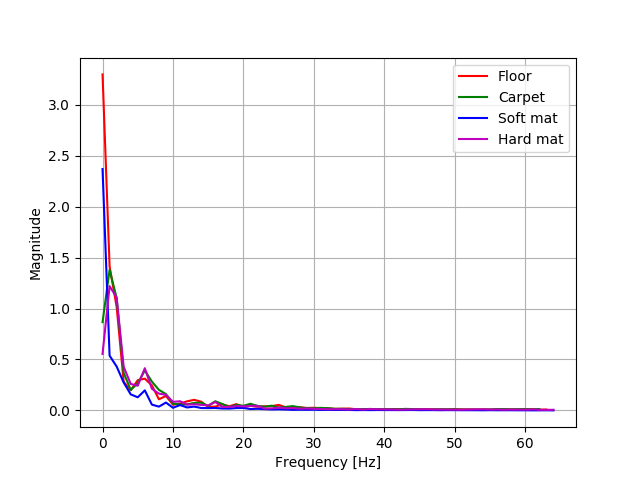
\includegraphics[width=1\linewidth]{Figures/fftz}
		\caption{Mean of 10 samples in z-direction}
		\label{fig:fftz}
	\end{subfigure}
	
	\caption[]{The figure showing the mean of each terrain different direction in frequency domain. (a) mean in the x-direction (b) mean in y-direction (c) in z-direction}
	\label{fig:fftxyz}
\end{figure}
\FloatBarrier

	
	
	
\section{Adding feature selection}
Even there are classifiers which outperform the other, there are still improvement potential. In the previous approach, the feature selection was not taken in account. The purpose of not using the feature selection was to see the performance without losing any features. In following experiment, the feature selection will be integrated on previous implementation to see if there any improvement. The modified implementation is shown in figure \ref{fig:approach2}, where the added component is marked as red. The filter and wrapper method will be used, and both are libraries provided by scikit-learn. The filter method will be removing features with low variance, while the wrapper method is recursive feature elimination and remove features to a desired number. A more detailed of each method can be found in appendix \ref{ap:featuresel}.

\paragraph{Removing features with low variance} \label{ap:variance}
This feature selection algorithm provided from Python removes all features whose variance does not meet some threshold. The default value will remove all features with the same values, which is most unlikely will occur in this experiment. Thus, in experiments the method will be removing feature when the variance is less than 0.2. 

\paragraph{Recursive feature elimination} \label{ap:rfe}
This feature selection algorithm will be using a supervised classifier to rank each features and remove features with low rank. The process is let a estimator to train of the features and weights thems. Features with smallest weights are pruned, and start to estimate with the currently features. This will be repeated until the desired number of features is reached.

	
\begin{figure}[h]
	\centering
	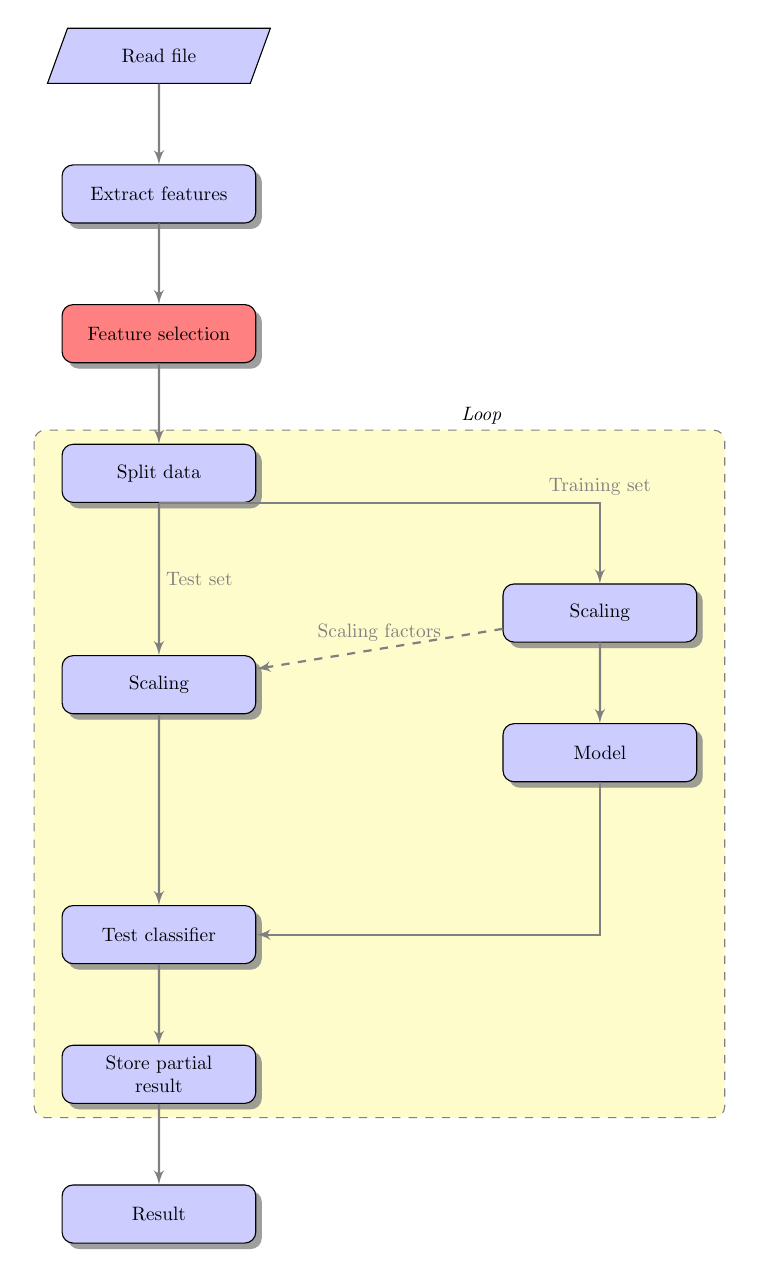
\begin{tikzpicture}[scale=0.7,transform shape]
		
		% Draw diagram elements
		%  \path \io{1}{Raw data};
		\path \io{2}{Read file};
		%  \path (p1.south)+(0,-1.5) \etape{2}{Extract steps};
		\path (p2.south)+(0.0,-2) \etape{3}{Extract features};
		\path (p3.south)+(0.0,-2) \etapeTre{11}{Feature selection};
		
		\path (p11.south)+(0.0,-2) \etape{4}{Split data};
		\path (p4.south)+(8,-2.0) \etape{5}{Scaling};
		\path (p5.south)+(0,-2) \etape{6}{Model};
		\path (p4.south)+(0,-3.3) \etape{9}{Scaling};
		\path (p9.south)+(0,-4.0) \etape{7}{Test classifier};		
		\path (p7.south)+(0,-2) \etape{10}{Store partial result};
		\path (p10.south)+(0,-2) \etape{8}{Result};
		
		%  \node [below=of p5] (p6-7) {};
		
		% Draw arrows between elements
		% \path [line] (p1.south) -- node [above] {} (p2);
		\path [line] (p2.south) -- node [above] {} (p3);
		\path [line] (p3.south) -- node [above] {} (p11);
		\path [line] (p11.south) -- node [above] {} (p4);
		\path [line] (p4.south) -| node [above] {Training set} (p5);
		
		\path [line] (p5.south) -- node [above] {} (p6);
		\path [line] (p6.south) |- node [above] {} (p7);
		\path [line] (p4.south) -- node [right] {Test set} (p9);
		\path [line] (p7.south) -- node [above] {} (p10);
		\path [line] (p10.south) -- node [above] {} (p8);
		\path [line] (p9.south) -- node [above] {} (p7);
		%  \path [line] (p5.south) -- node [above] {Feature} (p9);
		\path [line,dashed] (p5) -- node [above]{Scaling factors} (p9);
		\background{p3}{p4}{p5}{p10}{Loop} 
		
		\end{tikzpicture}
		
		\caption{Figure showing the new approach with added feature selection.} \label{fig:approach2}
	\end{figure}
\FloatBarrier
\newpage
\subsection{Results}
Table \ref{tab:exp2_1} shows the number of feature were removed for each sets. In table \ref{tab:exp2} shows the results for when feature selection is applied to the earlier learning approach and is compared previous implementation.	The five of top performing are marked with bold text, which is also be used in further experiments. 


\begin{table}[h]
	\centering
	\begin{tabular}{llll}
		\hline
		\textbf{Feature set} & \textbf{Old} & \textbf{Filter} & \textbf{Wrapper} \\ \hline
		Set 1 & 375 & 230 & 187 \\
		Set 2 & 21 & 8 & 10 \\
		Set 3 & 183 & 2 & 91 \\
		Set 4 & 24 & 11 & 12 \\
		Set 5 & 45 & 19 & 22 \\ \hline
	\end{tabular}
	\caption{Table showing new length of each features}
	\label{tab:exp2_1}
\end{table}
\FloatBarrier


\begin{table}[h]
	\centering
	\resizebox{\textwidth}{!} & \multicolumn{1}{l|}{{\color[HTML]{FE0000} 78\%}} & {\color[HTML]{FE0000} 81\%} \\ \cmidrule(l){2-5} 
			\multicolumn{1}{l|}{} & \multicolumn{1}{l|}{\textbf{Decision tree}} & \multicolumn{1}{l|}{\textbf{96\%}} & \multicolumn{1}{l|}{\textbf{96\%}} & {\color[HTML]{FE0000} 93\%} \\ \cmidrule(l){2-5} 
			\multicolumn{1}{l|}{} & \multicolumn{1}{l|}{KNN} & \multicolumn{1}{l|}{91\%} & \multicolumn{1}{l|}{{\color[HTML]{009901} 95\%}} & {\color[HTML]{009901} 93\%} \\ \cmidrule(l){2-5} 
			\multicolumn{1}{l|}{} & \multicolumn{1}{l|}{\textbf{Neural network}} & \multicolumn{1}{l|}{\textbf{96\%}} & \multicolumn{1}{l|}{{\color[HTML]{FE0000} 94\%}} & {\color[HTML]{FE0000} 95\%} \\ \cmidrule(l){2-5} 
			\multicolumn{1}{l|}{\multirow{-5}{*}{\textbf{\begin{tabular}[c]{@{}l@{}}Set one -\\ raw data\end{tabular}}}} & \multicolumn{1}{l|}{SVM} & \multicolumn{1}{l|}{93\%} & \multicolumn{1}{l|}{{\color[HTML]{FE0000} 91\%}} & {\color[HTML]{009901} 94\%} \\ \midrule
			\multicolumn{1}{l|}{} & \multicolumn{1}{l|}{Bayes Navies} & \multicolumn{1}{l|}{82\%} & \multicolumn{1}{l|}{{\color[HTML]{FE0000} 74\%}} & {\color[HTML]{009901} 84\%} \\ \cmidrule(l){2-5} 
			\multicolumn{1}{l|}{} & \multicolumn{1}{l|}{Decision tree} & \multicolumn{1}{l|}{84\%} & \multicolumn{1}{l|}{{\color[HTML]{FE0000} 79\%}} & {\color[HTML]{FE0000} 81\%} \\ \cmidrule(l){2-5} 
			\multicolumn{1}{l|}{} & \multicolumn{1}{l|}{KNN} & \multicolumn{1}{l|}{84\%} & \multicolumn{1}{l|}{{\color[HTML]{FE0000} 82\%}} & {\color[HTML]{FE0000} 82\%} \\ \cmidrule(l){2-5} 
			\multicolumn{1}{l|}{} & \multicolumn{1}{l|}{Neural network} & \multicolumn{1}{l|}{88\%} & \multicolumn{1}{l|}{{\color[HTML]{FE0000} 81\%}} & {\color[HTML]{FE0000} 84\%} \\ \cmidrule(l){2-5} 
			\multicolumn{1}{l|}{\multirow{-5}{*}{\begin{tabular}[c]{@{}l@{}}Set two - \\ statistical features in \\ time domain\end{tabular}}} & \multicolumn{1}{l|}{SVM} & \multicolumn{1}{l|}{85\%} & \multicolumn{1}{l|}{{\color[HTML]{FE0000} 80\%}} & {\color[HTML]{FE0000} 83\%} \\ \midrule
			\multicolumn{1}{l|}{} & \multicolumn{1}{l|}{Bayes Navies} & \multicolumn{1}{l|}{91\%} & \multicolumn{1}{l|}{{\color[HTML]{FE0000} 76\%}} & {\color[HTML]{FE0000} 94\%} \\ \cmidrule(l){2-5} 
			\multicolumn{1}{l|}{} & \multicolumn{1}{l|}{Decision tree} & \multicolumn{1}{l|}{82\%} & \multicolumn{1}{l|}{{\color[HTML]{FE0000} 76\%}} & {\color[HTML]{FE0000} 81\%} \\ \cmidrule(l){2-5} 
			\multicolumn{1}{l|}{} & \multicolumn{1}{l|}{KNN} & \multicolumn{1}{l|}{88\%} & \multicolumn{1}{l|}{{\color[HTML]{FE0000} 83\%}} & 88\% \\ \cmidrule(l){2-5} 
			\multicolumn{1}{l|}{} & \multicolumn{1}{l|}{Neural network} & \multicolumn{1}{l|}{93\%} & \multicolumn{1}{l|}{{\color[HTML]{FE0000} 78\%}} & {\color[HTML]{009901} 94\%} \\ \cmidrule(l){2-5} 
			\multicolumn{1}{l|}{\multirow{-5}{*}{\textbf{\begin{tabular}[c]{@{}l@{}}Set three - \\ complete frequency \\ domain\end{tabular}}}} & \multicolumn{1}{l|}{\textbf{SVM}} & \multicolumn{1}{l|}{93\%} & \multicolumn{1}{l|}{{\color[HTML]{FE0000} 79\%}} & {\color[HTML]{009901} \textbf{97\%}} \\ \midrule
			\multicolumn{1}{l|}{} & \multicolumn{1}{l|}{Bayes Navies} & \multicolumn{1}{l|}{81\%} & \multicolumn{1}{l|}{{\color[HTML]{FE0000} 75\%}} & {\color[HTML]{FE0000} 79\%} \\ \cmidrule(l){2-5} 
			\multicolumn{1}{l|}{} & \multicolumn{1}{l|}{Decision tree} & \multicolumn{1}{l|}{82\%} & \multicolumn{1}{l|}{82\%} & {\color[HTML]{FE0000} 81\%} \\ \cmidrule(l){2-5} 
			\multicolumn{1}{l|}{} & \multicolumn{1}{l|}{KNN} & \multicolumn{1}{l|}{84\%} & \multicolumn{1}{l|}{{\color[HTML]{009901} 85\%}} & {\color[HTML]{009901} 86\%} \\ \cmidrule(l){2-5} 
			\multicolumn{1}{l|}{} & \multicolumn{1}{l|}{Neural network} & \multicolumn{1}{l|}{88\%} & \multicolumn{1}{l|}{{\color[HTML]{FE0000} 84\%}} & {\color[HTML]{009901} 90\%} \\ \cmidrule(l){2-5} 
			\multicolumn{1}{l|}{\multirow{-5}{*}{\textbf{\begin{tabular}[c]{@{}l@{}}Set four - \\ staticial features in \\ frequency domain\end{tabular}}}} & \multicolumn{1}{l|}{SVM} & \multicolumn{1}{l|}{86\%} & \multicolumn{1}{l|}{{\color[HTML]{FE0000} 82\%}} & {\color[HTML]{009901} 86\%} \\ \midrule
			\multicolumn{1}{l|}{} & \multicolumn{1}{l|}{Bayes Navies} & \multicolumn{1}{l|}{82\%} & \multicolumn{1}{l|}{{\color[HTML]{FE0000} 74\%}} & {\color[HTML]{009901} 84\%} \\ \cmidrule(l){2-5} 
			\multicolumn{1}{l|}{} & \multicolumn{1}{l|}{Decision tree} & \multicolumn{1}{l|}{80\%} & \multicolumn{1}{l|}{{\color[HTML]{009901} 82\%}} & {\color[HTML]{009901} 82\%} \\ \cmidrule(l){2-5} 
			\multicolumn{1}{l|}{} & \multicolumn{1}{l|}{\textbf{KNN}} & \multicolumn{1}{l|}{84\%} & \multicolumn{1}{l|}{{\color[HTML]{009901} 86\%}} & {\color[HTML]{009901} \textbf{86\%}} \\ \cmidrule(l){2-5} 
			\multicolumn{1}{l|}{} & \multicolumn{1}{l|}{Neural network} & \multicolumn{1}{l|}{89\%} & \multicolumn{1}{l|}{{\color[HTML]{FE0000} 81\%}} & {\color[HTML]{FE0000} 85\%} \\ \cmidrule(l){2-5} 
			\multicolumn{1}{l|}{\multirow{-5}{*}{\textbf{\begin{tabular}[c]{@{}l@{}}Set five - \\ set 2,4\end{tabular}}}} & \multicolumn{1}{l|}{SVM} & \multicolumn{1}{l|}{86\%} & \multicolumn{1}{l|}{{\color[HTML]{FE0000} 83\%}} & {\color[HTML]{009901} 84\%} \\ \bottomrule
		\end{tabular}%
	}
	\caption{Table showing the results after following integrating  feature selection to the learning approach}
	\label{tab:exp2}
\end{table}
\FloatBarrier
	
\subsection{Analysis}
From table \ref{tab:exp2}, one can see that adding the feature selection has decreased performance of most classifiers. The filter method on feature set three gave poorest performance, as it can be seen it also only has two feature from table \ref{tab:exp2_1}. The wrapper selection, on the other hand, also have some classifier which performed less accurately, but the difference between old result is less than filter. Some of classifier has improved significant, particularly the SVM with feature set three with 97\% accuracy which is also top performed classifier.
\\
\\
It will be interesting to investigate the feature selected from each method. However, this thesis will only present features from the highest accuracy which is wrapper on feature set 3. Other selected features can be seen in appendix \ref{ap:self}. Thus, a mean of feature in time domain with mean is shown in figure \ref{fig:wrapperset5}. It can be seen big variance between the first features. When the frequency is higher less variance is it between each features.


\begin{figure} [h]
	\centering
	\begin{subfigure}[b]{\textwidth}
		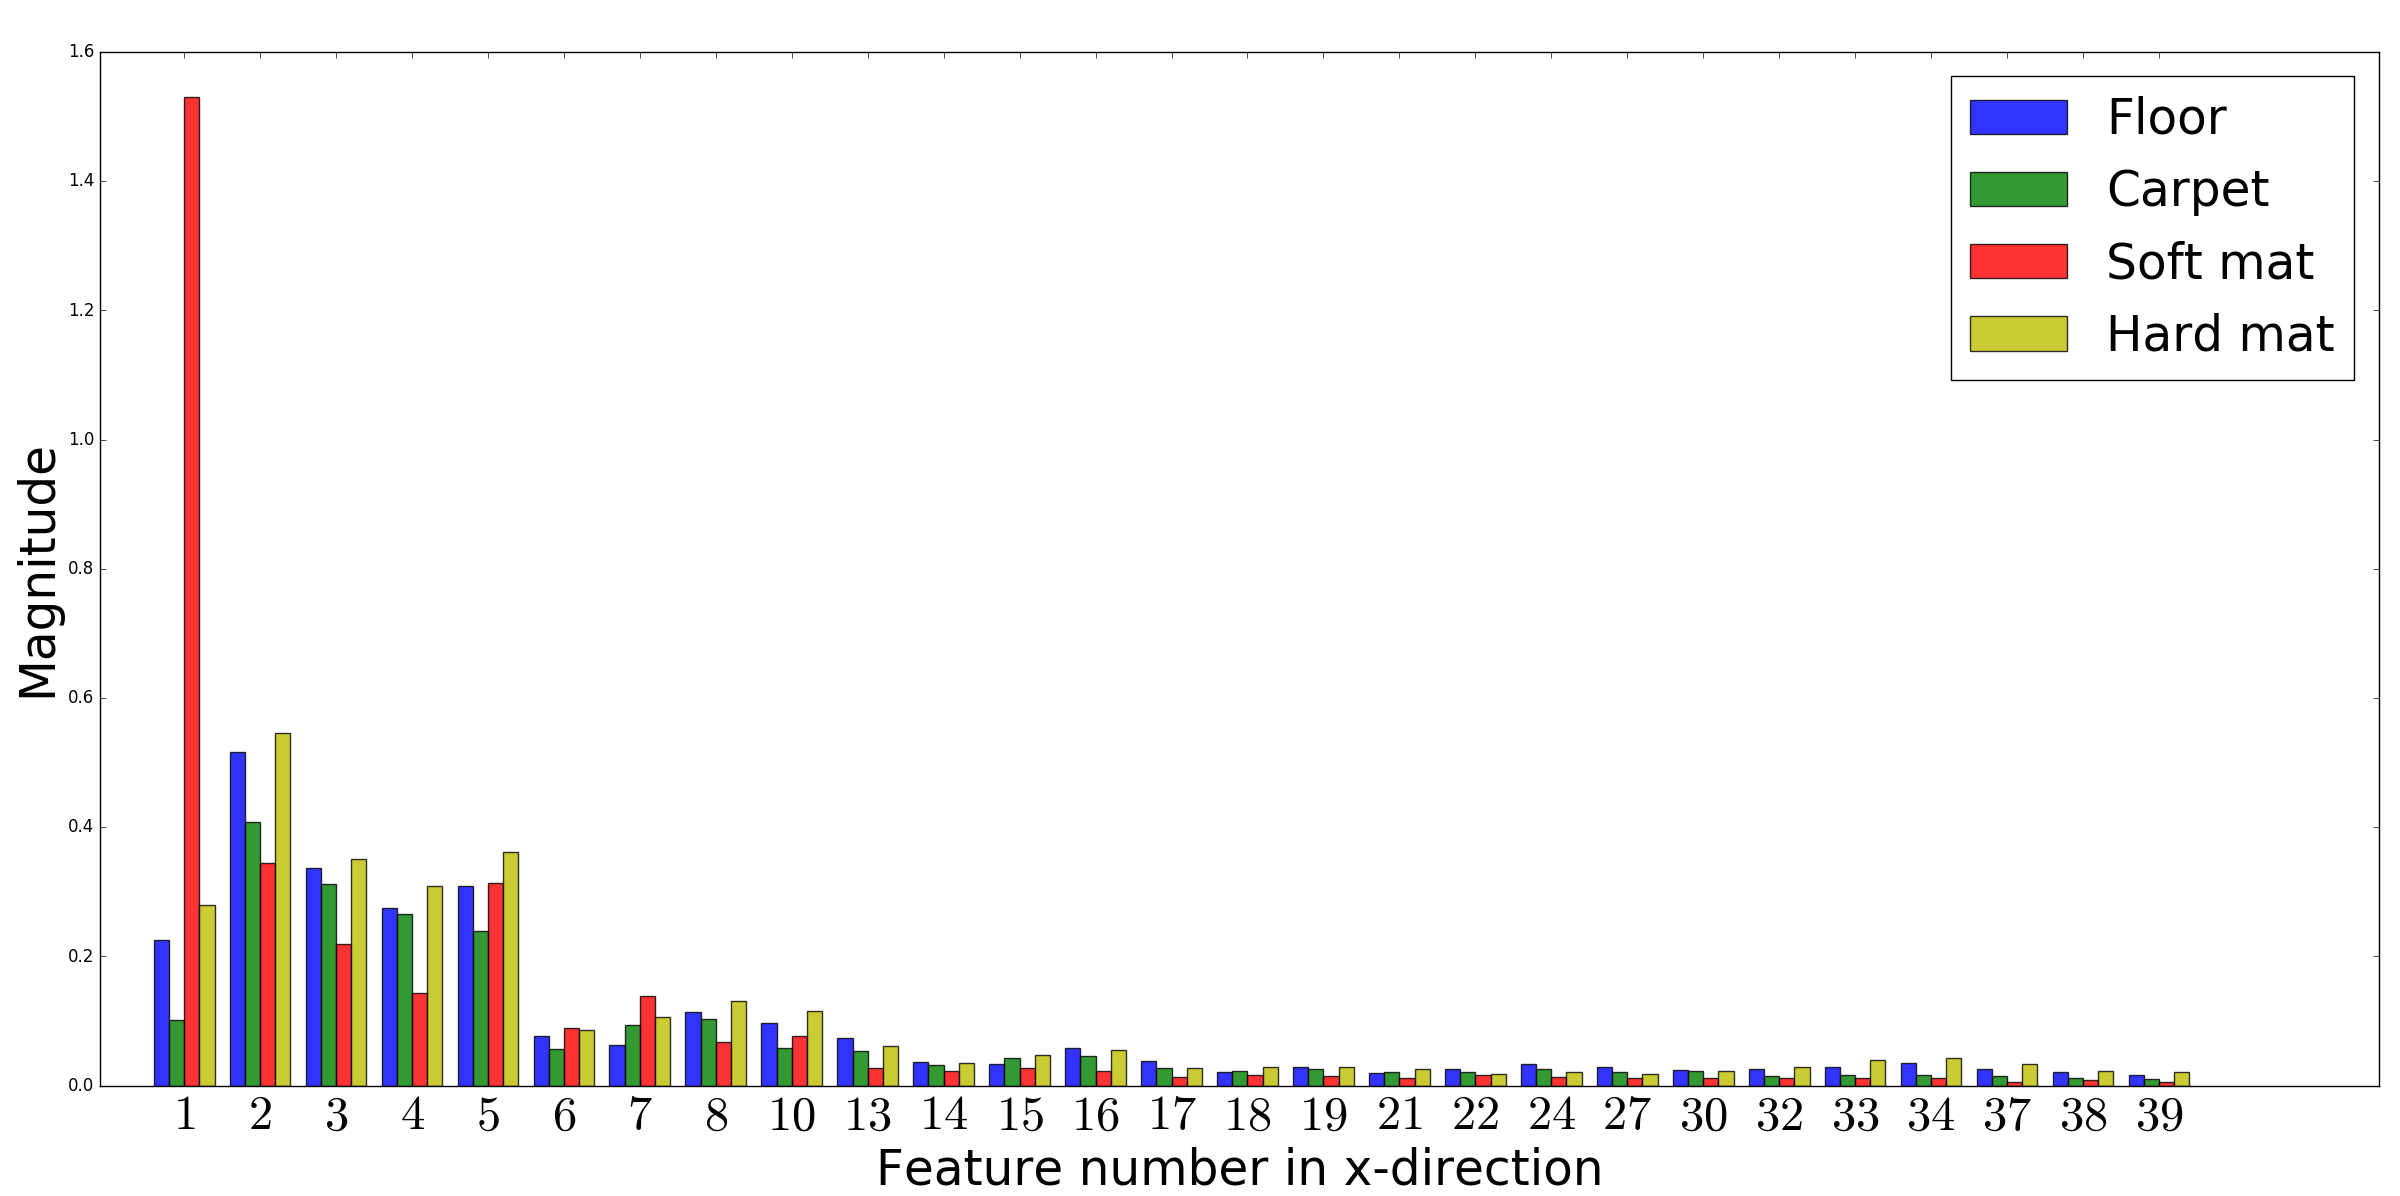
\includegraphics[width=\textwidth,height=\textheight,keepaspectratio]{Figures/featureselx}
		\caption{Features in x-direction}
		\label{fig:featurex} 
	\end{subfigure}
	
	\begin{subfigure}[b]{\textwidth}
		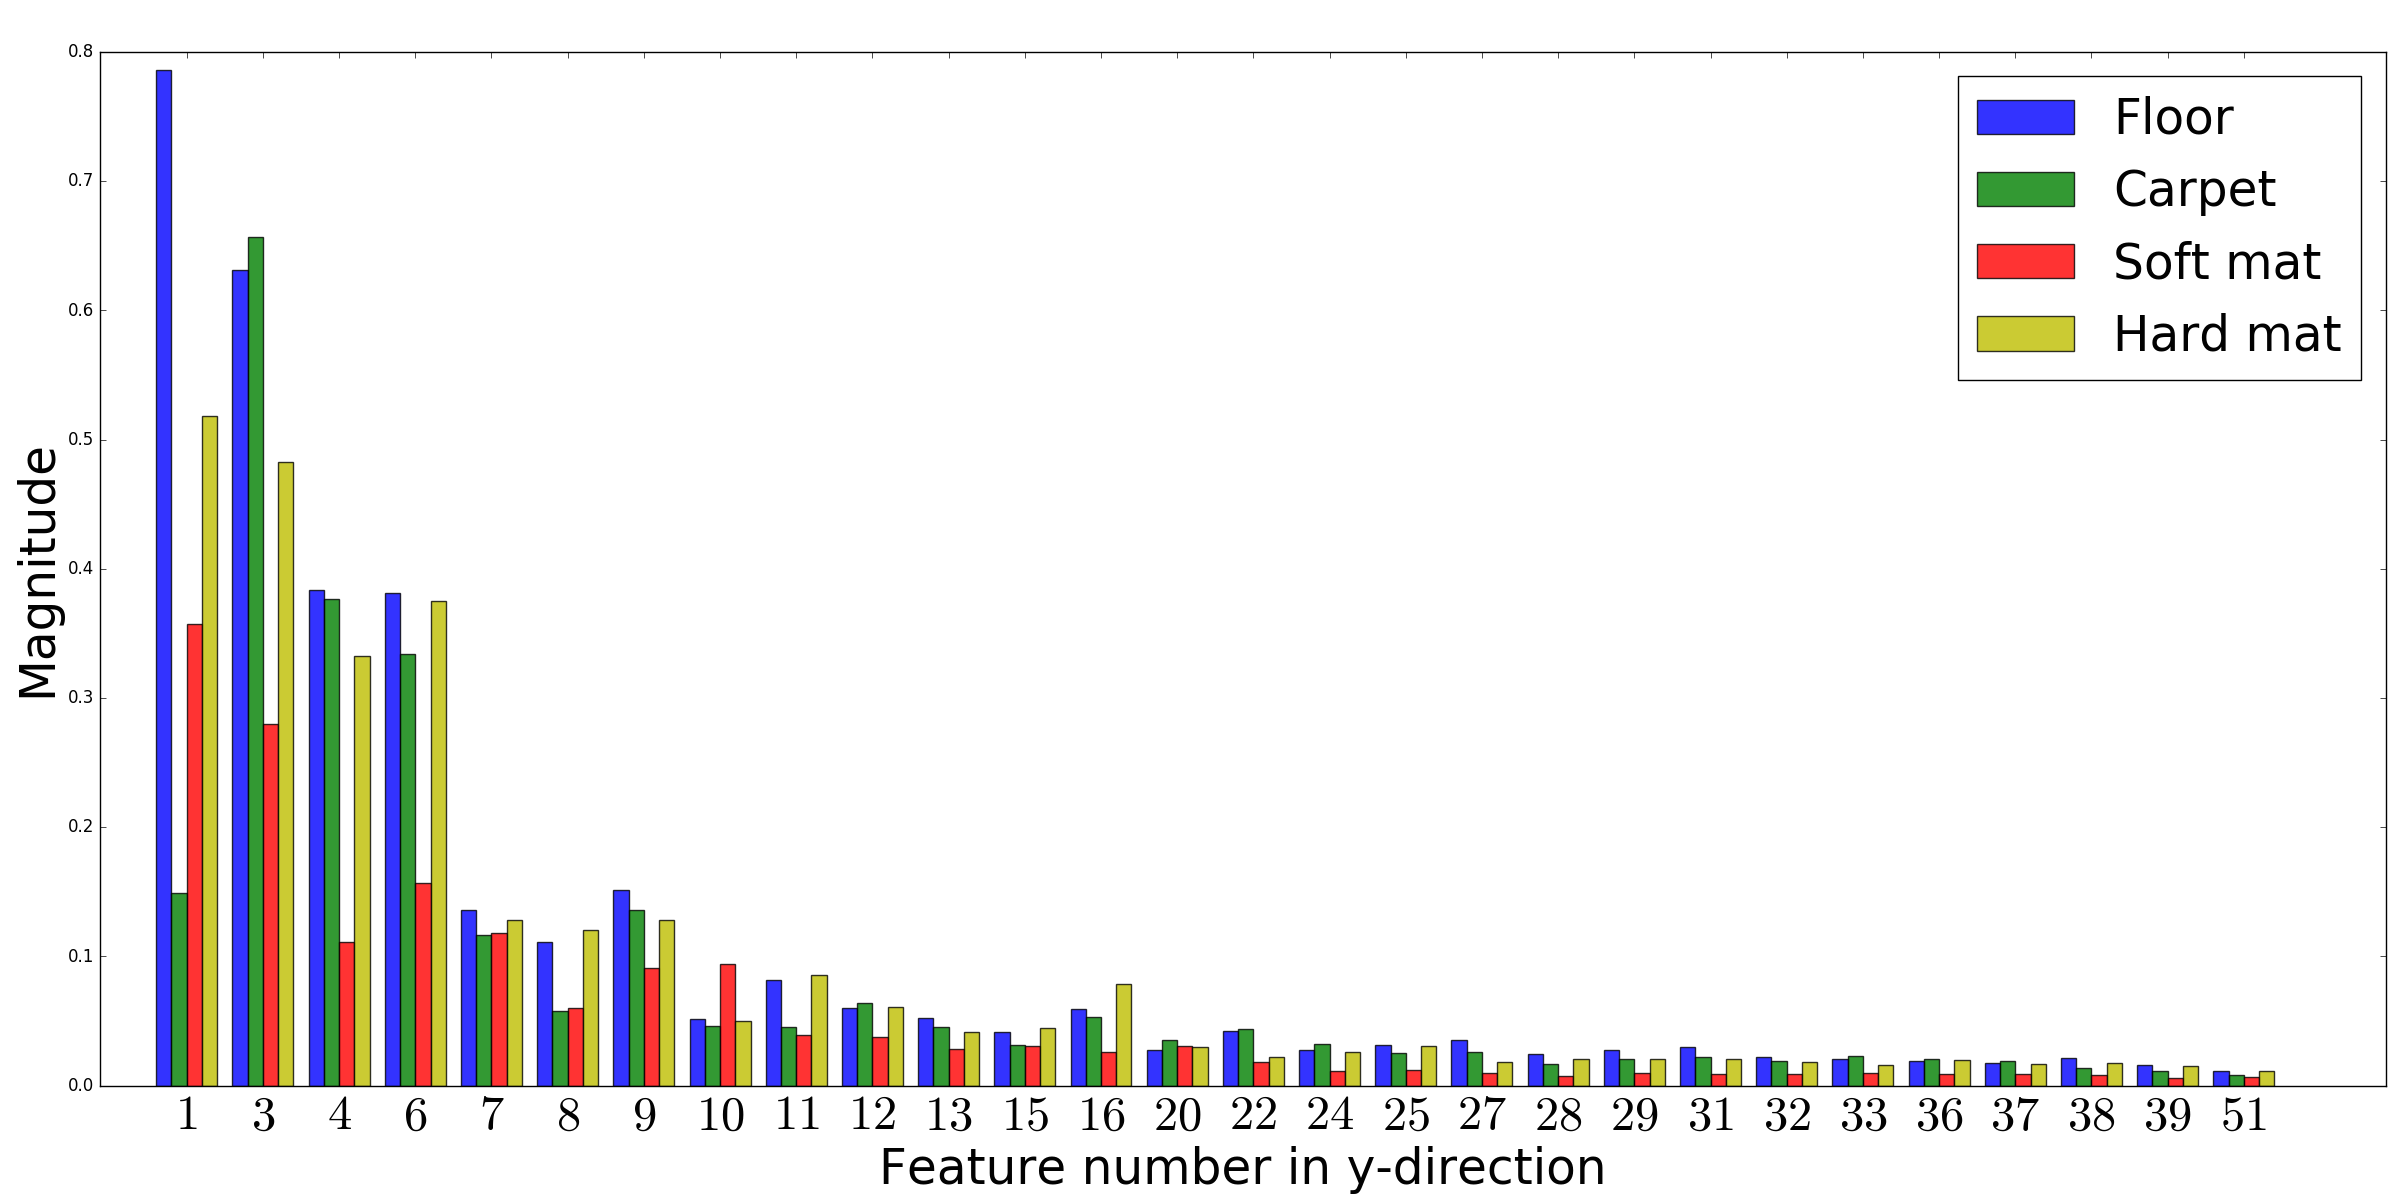
\includegraphics[width=\textwidth,height=\textheight,keepaspectratio]{Figures/featuresely}
		\caption{Features in y-direction}
		\label{fig:featurey}
	\end{subfigure}
	
	\begin{subfigure}[h]{\textwidth}
		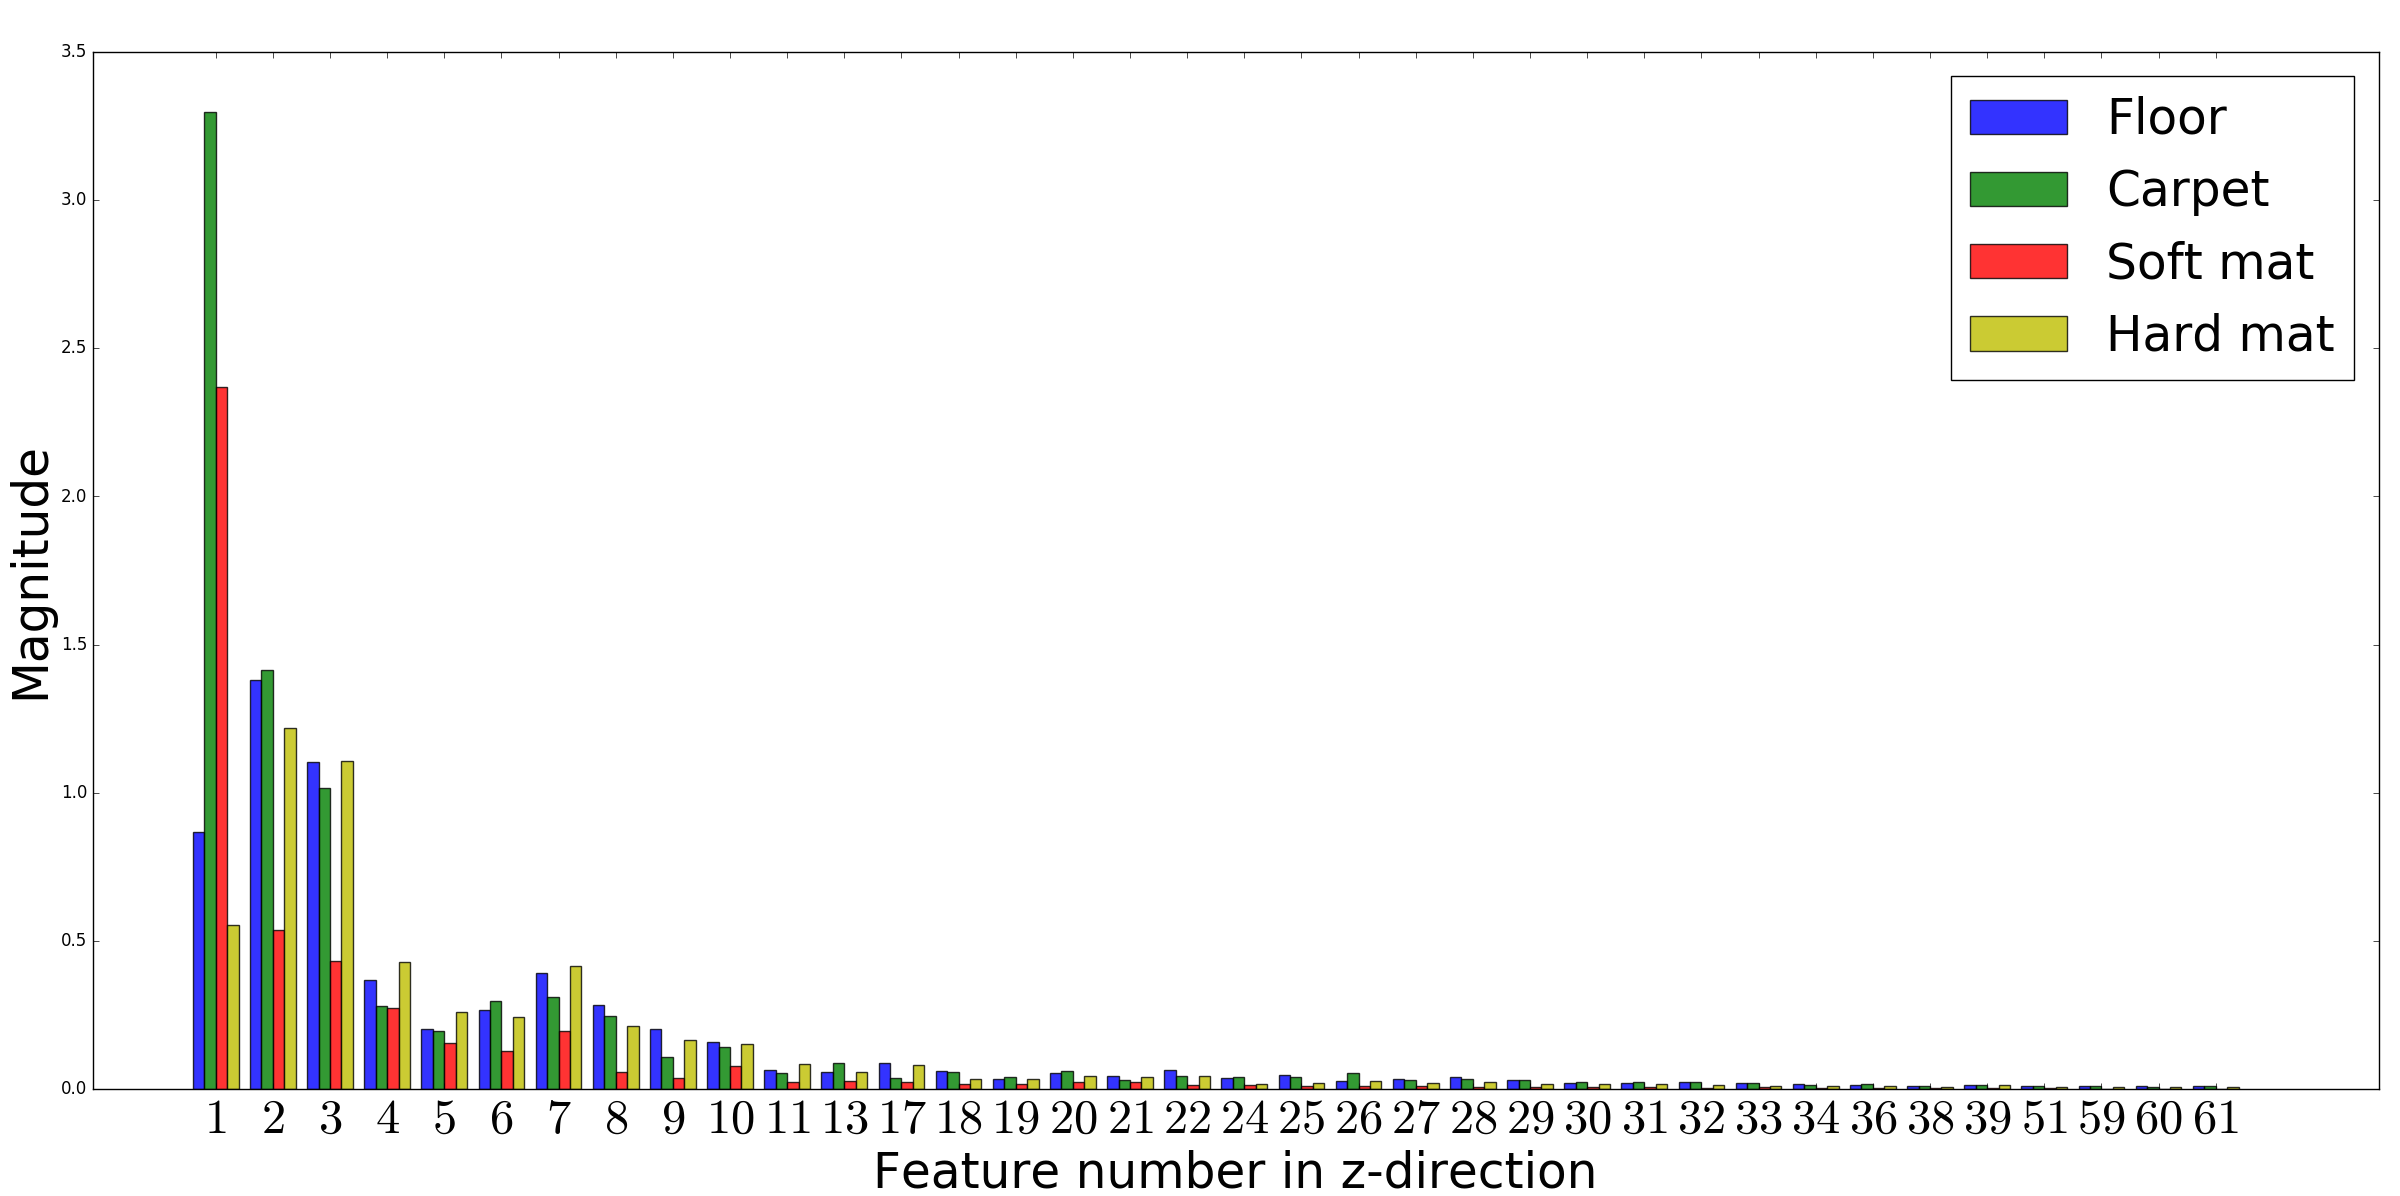
\includegraphics[width=\textwidth,height=\textheight,keepaspectratio]{Figures/featureselz}
		\caption{Features in z-direction}
		\label{fig:featurez}
	\end{subfigure}

	\caption{Figure showing comparison of each features for each terrain on feature set three}
	\label{fig:wrapperset5}
\end{figure}
\FloatBarrier

\section{Cross validation with unseen data} \label{seq:crossunseen}
Note that the k-fold validation test using always use the same single set both for training and testing, which make it referring to themselves has the risk of not generalizing the classifier. In this case results from \ref{tab:exp2} only gives an estimation on how well a classifier is, but does not tell how well it predict on unseen data. One way to avoid this issue is make the training and testing set independent to each other, so the prediction will be based on new and unseen data \cite{26b23e912c654fe4b7478fd910130195}. The following experiment will be using two highest performed classifier shown in \ref{tab:exp2}. As there are three shared second best classifier, all of them will be in further experiments. Additionally, Neural Network without selection method with feature set five achieved a satisfied result which will also be further investigated. The reason is among the four best performed classifier is only using either the entire raw data or frequency domain. Thus, it will be interesting to compare a classifier with extracted features.
\\
\\
In this experiment 50 new samples for each terrain is collected. In the cross validation it will use the old dataset as training set, while the new collected samples will be used as test file. The cross validation is still LOOCV. To achieve a reliable performance estimation can be done by run the cross-validation multiple times \cite{Refaeilzadeh2009}. Thus, the training and test set will be randomly shuffled before each round of cross-validation, and this will be done five times.

	\begin{enumerate}
		\item SVM with wrapper and use feature set two
		\item Neural Network and use feature set one.
		\item Decision tree with feature set one
		\item Decision tree with filter and use feature set one
		\item KNN with wrapper and feature set five
	\end{enumerate}

\subsection{Results}
An overview of the performance is shown as box plot in figure \ref{fig:boxexp}. Again, the top performing is the SVM, while the other classifier has decreased their accuracy in their performance.

\begin{figure}[h]
	\centering
	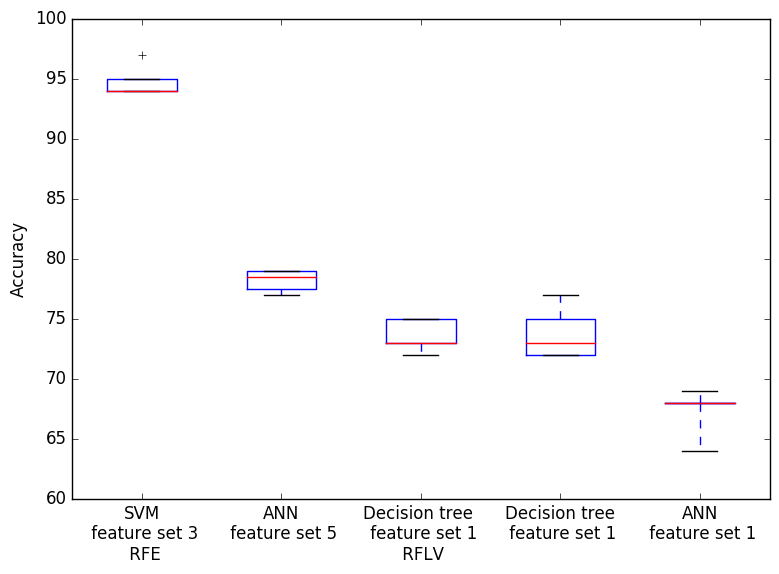
\includegraphics[width=\textwidth,height=\textheight,keepaspectratio]{Figures/compareUnseen}
	\caption{Figure showing data stream from sensor when the robot walked from floor to carpet.}
	\label{fig:boxexp}
\end{figure}
\FloatBarrier
\subsection{Analysis}
In this section it will present a more detailed of each classifier. The order is starting with the best performed classifier and bad in the end.
\newpage
\subsubsection{SVM - Wrapper - Feature set two}
In the table \ref{svmexp} showing accuracy of each run. The average performance of the classifier is at 94.8\%. The classifier easily predicts floor, carpet, and soft mat, while it has some difficulties to predict hard mat. When the robot is on hard mat it has an average predicting correct of 84\%, it tend to predict it as carpet. Cause of hard mat tend to predict other terrains, the f-score for floor and carpet is decreased a little as seen in table \ref{fscoresvm}. The hard mat and carpet has relative equally f-score. However the carpet got a lower recall, but higher precision, while the hard mat got higher recall, but lower precision. 

\begin{table}[h]
	\centering
	\begin{tabular}{@{}llllll@{}}
		\toprule
		\multirow{2}{*}{\textbf{Run}} & \multirow{2}{*}{\textbf{Accuracy}} & \multicolumn{4}{c}{\textbf{Confusion matrix}} \\ \cmidrule(l){3-6} 
			&  & \multicolumn{1}{l|}{\textbf{Floor}} & \multicolumn{1}{l|}{\textbf{Carpet}} & \multicolumn{1}{l|}{\textbf{Soft mat}} & \textbf{Hard mat} \\ \midrule
			\multicolumn{1}{l|}{\multirow{4}{*}{1}} & \multicolumn{1}{l|}{\multirow{4}{*}{94\%}} & \multicolumn{1}{l|}{50} & \multicolumn{1}{l|}{0} & \multicolumn{1}{l|}{0} & 0 \\ \cmidrule(l){3-6} 
			\multicolumn{1}{l|}{} & \multicolumn{1}{l|}{} & \multicolumn{1}{l|}{3} & \multicolumn{1}{l|}{47} & \multicolumn{1}{l|}{0} & 0 \\ \cmidrule(l){3-6} 
			\multicolumn{1}{l|}{} & \multicolumn{1}{l|}{} & \multicolumn{1}{l|}{0} & \multicolumn{1}{l|}{0} & \multicolumn{1}{l|}{50} & 0 \\ \cmidrule(l){3-6} 
			\multicolumn{1}{l|}{} & \multicolumn{1}{l|}{} & \multicolumn{1}{l|}{2} & \multicolumn{1}{l|}{7} & \multicolumn{1}{l|}{0} & 41 \\ \midrule
			\multicolumn{1}{l|}{\multirow{4}{*}{2}} & \multicolumn{1}{l|}{\multirow{4}{*}{97\%}} & \multicolumn{1}{l|}{50} & \multicolumn{1}{l|}{0} & \multicolumn{1}{l|}{0} & 0 \\ \cmidrule(l){3-6} 
			\multicolumn{1}{l|}{} & \multicolumn{1}{l|}{} & \multicolumn{1}{l|}{2} & \multicolumn{1}{l|}{48} & \multicolumn{1}{l|}{0} & 0 \\ \cmidrule(l){3-6} 
			\multicolumn{1}{l|}{} & \multicolumn{1}{l|}{} & \multicolumn{1}{l|}{0} & \multicolumn{1}{l|}{0} & \multicolumn{1}{l|}{50} & 0 \\ \cmidrule(l){3-6} 
			\multicolumn{1}{l|}{} & \multicolumn{1}{l|}{} & \multicolumn{1}{l|}{2} & \multicolumn{1}{l|}{1} & \multicolumn{1}{l|}{0} & 47 \\ \midrule
			\multicolumn{1}{l|}{\multirow{4}{*}{3}} & \multicolumn{1}{l|}{\multirow{4}{*}{94\%}} & \multicolumn{1}{l|}{50} & \multicolumn{1}{l|}{0} & \multicolumn{1}{l|}{0} & 0 \\ \cmidrule(l){3-6} 
			\multicolumn{1}{l|}{} & \multicolumn{1}{l|}{} & \multicolumn{1}{l|}{2} & \multicolumn{1}{l|}{48} & \multicolumn{1}{l|}{0} & 0 \\ \cmidrule(l){3-6} 
			\multicolumn{1}{l|}{} & \multicolumn{1}{l|}{} & \multicolumn{1}{l|}{0} & \multicolumn{1}{l|}{0} & \multicolumn{1}{l|}{50} & 0 \\ \cmidrule(l){3-6} 
			\multicolumn{1}{l|}{} & \multicolumn{1}{l|}{} & \multicolumn{1}{l|}{2} & \multicolumn{1}{l|}{7} & \multicolumn{1}{l|}{0} & 41 \\ \midrule
			\multicolumn{1}{l|}{\multirow{4}{*}{4}} & \multicolumn{1}{l|}{\multirow{4}{*}{94\%}} & \multicolumn{1}{l|}{50} & \multicolumn{1}{l|}{0} & \multicolumn{1}{l|}{0} & 0 \\ \cmidrule(l){3-6} 
			\multicolumn{1}{l|}{} & \multicolumn{1}{l|}{} & \multicolumn{1}{l|}{2} & \multicolumn{1}{l|}{48} & \multicolumn{1}{l|}{0} & 0 \\ \cmidrule(l){3-6} 
			\multicolumn{1}{l|}{} & \multicolumn{1}{l|}{} & \multicolumn{1}{l|}{0} & \multicolumn{1}{l|}{0} & \multicolumn{1}{l|}{50} & 0 \\ \cmidrule(l){3-6} 
			\multicolumn{1}{l|}{} & \multicolumn{1}{l|}{} & \multicolumn{1}{l|}{2} & \multicolumn{1}{l|}{8} & \multicolumn{1}{l|}{0} & 40 \\ \midrule
			\multicolumn{1}{l|}{\multirow{4}{*}{5}} & \multicolumn{1}{l|}{\multirow{4}{*}{95\%}} & \multicolumn{1}{l|}{50} & \multicolumn{1}{l|}{0} & \multicolumn{1}{l|}{0} & 0 \\ \cmidrule(l){3-6} 
			\multicolumn{1}{l|}{} & \multicolumn{1}{l|}{} & \multicolumn{1}{l|}{1} & \multicolumn{1}{l|}{49} & \multicolumn{1}{l|}{0} & 0 \\ \cmidrule(l){3-6} 
			\multicolumn{1}{l|}{} & \multicolumn{1}{l|}{} & \multicolumn{1}{l|}{0} & \multicolumn{1}{l|}{0} & \multicolumn{1}{l|}{50} & 0 \\ \cmidrule(l){3-6} 
			\multicolumn{1}{l|}{} & \multicolumn{1}{l|}{} & \multicolumn{1}{l|}{2} & \multicolumn{1}{l|}{7} & \multicolumn{1}{l|}{0} & 41 \\ \bottomrule
		\end{tabular}
		\caption{Table showing the accuracy and confusion matrix for SVM with wrapper and feature set two. The row show the actual terrains and the columns is predicted terrain}
		\label{svmexp}
	\end{table}
	\FloatBarrier
	\begin{table}[h]
		\centering
		\begin{tabular}{@{}llllll@{}}
			\toprule
			\multirow{2}{*}{\textbf{Terrain}} & \multicolumn{5}{c}{\textbf{Run}} \\ \cmidrule(l){2-6} 
			& \multicolumn{1}{l|}{\textbf{1}} & \multicolumn{1}{l|}{\textbf{2}} & \multicolumn{1}{l|}{\textbf{3}} & \multicolumn{1}{l|}{\textbf{4}} & \textbf{5} \\ \midrule
			\multicolumn{1}{l|}{Floor} & \multicolumn{1}{l|}{100\%} & \multicolumn{1}{l|}{100\%} & \multicolumn{1}{l|}{100\%} & \multicolumn{1}{l|}{100\%} & 100\% \\ \midrule
			\multicolumn{1}{l|}{Carpet} & \multicolumn{1}{l|}{94\%} & \multicolumn{1}{l|}{96\%} & \multicolumn{1}{l|}{96\%} & \multicolumn{1}{l|}{96\%} & 98\% \\ \midrule
			\multicolumn{1}{l|}{Soft mat} & \multicolumn{1}{l|}{100\%} & \multicolumn{1}{l|}{100\%} & \multicolumn{1}{l|}{100\%} & \multicolumn{1}{l|}{100\%} & 100\% \\ \midrule
			\multicolumn{1}{l|}{Hard mat} & \multicolumn{1}{l|}{82\%} & \multicolumn{1}{l|}{94\%} & \multicolumn{1}{l|}{82\%} & \multicolumn{1}{l|}{80\%} & 82\% \\ \bottomrule
		\end{tabular}
		\caption{Table shows precision of SVM}
		\label{pressvm}
	\end{table}
	\FloatBarrier
	
	\begin{table}[h]
		\centering
		\begin{tabular}{@{}llllll@{}}
			\toprule
			\multirow{2}{*}{\textbf{Terrain}} & \multicolumn{5}{c}{\textbf{Run}} \\ \cmidrule(l){2-6} 
			& \multicolumn{1}{l|}{\textbf{1}} & \multicolumn{1}{l|}{\textbf{2}} & \multicolumn{1}{l|}{\textbf{3}} & \multicolumn{1}{l|}{\textbf{4}} & \textbf{5} \\ \midrule
			\multicolumn{1}{l|}{Floor} & \multicolumn{1}{l|}{90.9\%} & \multicolumn{1}{l|}{92.6\%} & \multicolumn{1}{l|}{92.6\%} & \multicolumn{1}{l|}{92.6\%} & 87.5\% \\ \midrule
			\multicolumn{1}{l|}{Carpet} & \multicolumn{1}{l|}{87\%} & \multicolumn{1}{l|}{98\%} & \multicolumn{1}{l|}{87.2\%} & \multicolumn{1}{l|}{85.7\%} & 98\% \\ \midrule
			\multicolumn{1}{l|}{Soft mat} & \multicolumn{1}{l|}{100\%} & \multicolumn{1}{l|}{100\%} & \multicolumn{1}{l|}{100\%} & \multicolumn{1}{l|}{100\%} & 100\% \\ \midrule
			\multicolumn{1}{l|}{Hard mat} & \multicolumn{1}{l|}{100\%} & \multicolumn{1}{l|}{100\%} & \multicolumn{1}{l|}{100\%} & \multicolumn{1}{l|}{100\%} & 100\% \\ \bottomrule
		\end{tabular}
		\caption{Table shows recall of SVM}
		\label{recallsvm}
	\end{table}
	\FloatBarrier
	
	\begin{table}[h]
		\centering
		\begin{tabular}{@{}llllll@{}}
			\toprule
			\multirow{2}{*}{\textbf{Terrain}} & \multicolumn{5}{c}{\textbf{Run}} \\ \cmidrule(l){2-6} 
			& \multicolumn{1}{l|}{\textbf{1}} & \multicolumn{1}{l|}{\textbf{2}} & \multicolumn{1}{l|}{\textbf{3}} & \multicolumn{1}{l|}{\textbf{4}} & \textbf{5} \\ \midrule
			\multicolumn{1}{l|}{Floor} & \multicolumn{1}{l|}{95.2\%} & \multicolumn{1}{l|}{96.2\%} & \multicolumn{1}{l|}{96.2\%} & \multicolumn{1}{l|}{96.2\%} & 98\% \\ \midrule
			\multicolumn{1}{l|}{Carpet} & \multicolumn{1}{l|}{90.4\%} & \multicolumn{1}{l|}{97\%} & \multicolumn{1}{l|}{91.4\%} & \multicolumn{1}{l|}{90.6\%} & 97\% \\ \midrule
			\multicolumn{1}{l|}{Soft mat} & \multicolumn{1}{l|}{100\%} & \multicolumn{1}{l|}{100\%} & \multicolumn{1}{l|}{100\%} & \multicolumn{1}{l|}{100\%} & 100\% \\ \midrule
			\multicolumn{1}{l|}{Hard mat} & \multicolumn{1}{l|}{90.1\%} & \multicolumn{1}{l|}{96.9\%} & \multicolumn{1}{l|}{90.1\%} & \multicolumn{1}{l|}{88\%} & 90.1\% \\ \bottomrule
		\end{tabular}
		\caption{Table shows f-score of SVM}
		\label{fscoresvm}
	\end{table}
	\FloatBarrier
\newpage

\subsubsection{Neuarl Network - Feature set one}
In the table \ref{nn2} showing accuracy of each run. The average performance of predicting unseen data has an accuracy of 67.4\%, and compared to the old result from \ref{tab:exp2} it has decreased with 28.6\%. It has no difficulties of predicting soft mat and carpet. However, the carpet has a low recall cause of when the robot is on either floor or hard mat, it tend to predict it as carpet. Most difficult is predicting the hard mat, which has an average precision on 21.2\%. Second hard terrain to predict is the floor with a precision of 49.6\%. Floor and hard mat tend to predict it as carpet, which is also why the carpet had low recall under 50\%. However, the classifier does predict correct when the robot is on carpet with a precision at least 94\%.


	\begin{table}[h]
		\centering
		\begin{tabular}{@{}llllll@{}}
			\toprule
			\multirow{2}{*}{\textbf{Run}} & \multirow{2}{*}{\textbf{Accuracy}} & \multicolumn{4}{c}{\textbf{Confusion matrix}} \\ \cmidrule(l){3-6} 
			&  & \multicolumn{1}{l|}{\textbf{Floor}} & \multicolumn{1}{l|}{\textbf{Carpet}} & \multicolumn{1}{l|}{\textbf{Soft mat}} & \textbf{Hard mat} \\ \midrule
			\multicolumn{1}{l|}{\multirow{4}{*}{1}} & \multicolumn{1}{l|}{\multirow{4}{*}{68\%}} & \multicolumn{1}{l|}{25} & \multicolumn{1}{l|}{25} & \multicolumn{1}{l|}{0} & 0 \\ \cmidrule(l){3-6} 
			\multicolumn{1}{l|}{} & \multicolumn{1}{l|}{} & \multicolumn{1}{l|}{1} & \multicolumn{1}{l|}{49} & \multicolumn{1}{l|}{0} & 0 \\ \cmidrule(l){3-6} 
			\multicolumn{1}{l|}{} & \multicolumn{1}{l|}{} & \multicolumn{1}{l|}{0} & \multicolumn{1}{l|}{0} & \multicolumn{1}{l|}{50} & 0 \\ \cmidrule(l){3-6} 
			\multicolumn{1}{l|}{} & \multicolumn{1}{l|}{} & \multicolumn{1}{l|}{11} & \multicolumn{1}{l|}{28} & \multicolumn{1}{l|}{0} & 11 \\ \midrule
			\multicolumn{1}{l|}{\multirow{4}{*}{2}} & \multicolumn{1}{l|}{\multirow{4}{*}{68\%}} & \multicolumn{1}{l|}{26} & \multicolumn{1}{l|}{24} & \multicolumn{1}{l|}{0} & 0 \\ \cmidrule(l){3-6} 
			\multicolumn{1}{l|}{} & \multicolumn{1}{l|}{} & \multicolumn{1}{l|}{1} & \multicolumn{1}{l|}{48} & \multicolumn{1}{l|}{0} & 1 \\ \cmidrule(l){3-6} 
			\multicolumn{1}{l|}{} & \multicolumn{1}{l|}{} & \multicolumn{1}{l|}{0} & \multicolumn{1}{l|}{0} & \multicolumn{1}{l|}{50} & 0 \\ \cmidrule(l){3-6} 
			\multicolumn{1}{l|}{} & \multicolumn{1}{l|}{} & \multicolumn{1}{l|}{9} & \multicolumn{1}{l|}{30} & \multicolumn{1}{l|}{0} & 11 \\ \midrule
			\multicolumn{1}{l|}{\multirow{4}{*}{3}} & \multicolumn{1}{l|}{\multirow{4}{*}{64\%}} & \multicolumn{1}{l|}{20} & \multicolumn{1}{l|}{30} & \multicolumn{1}{l|}{0} & 0 \\ \cmidrule(l){3-6} 
			\multicolumn{1}{l|}{} & \multicolumn{1}{l|}{} & \multicolumn{1}{l|}{0} & \multicolumn{1}{l|}{48} & \multicolumn{1}{l|}{0} & 2 \\ \cmidrule(l){3-6} 
			\multicolumn{1}{l|}{} & \multicolumn{1}{l|}{} & \multicolumn{1}{l|}{0} & \multicolumn{1}{l|}{0} & \multicolumn{1}{l|}{50} & 0 \\ \cmidrule(l){3-6} 
			\multicolumn{1}{l|}{} & \multicolumn{1}{l|}{} & \multicolumn{1}{l|}{11} & \multicolumn{1}{l|}{29} & \multicolumn{1}{l|}{0} & 10 \\ \midrule
			\multicolumn{1}{l|}{\multirow{4}{*}{4}} & \multicolumn{1}{l|}{\multirow{4}{*}{68\%}} & \multicolumn{1}{l|}{27} & \multicolumn{1}{l|}{23} & \multicolumn{1}{l|}{0} & 0 \\ \cmidrule(l){3-6} 
			\multicolumn{1}{l|}{} & \multicolumn{1}{l|}{} & \multicolumn{1}{l|}{0} & \multicolumn{1}{l|}{49} & \multicolumn{1}{l|}{0} & 1 \\ \cmidrule(l){3-6} 
			\multicolumn{1}{l|}{} & \multicolumn{1}{l|}{} & \multicolumn{1}{l|}{0} & \multicolumn{1}{l|}{0} & \multicolumn{1}{l|}{50} & 0 \\ \cmidrule(l){3-6} 
			\multicolumn{1}{l|}{} & \multicolumn{1}{l|}{} & \multicolumn{1}{l|}{9} & \multicolumn{1}{l|}{32} & \multicolumn{1}{l|}{0} & 9 \\ \midrule
			\multicolumn{1}{l|}{\multirow{4}{*}{5}} & \multicolumn{1}{l|}{\multirow{4}{*}{69\%}} & \multicolumn{1}{l|}{26} & \multicolumn{1}{l|}{24} & \multicolumn{1}{l|}{0} & 0 \\ \cmidrule(l){3-6} 
			\multicolumn{1}{l|}{} & \multicolumn{1}{l|}{} & \multicolumn{1}{l|}{0} & \multicolumn{1}{l|}{49} & \multicolumn{1}{l|}{0} & 1 \\ \cmidrule(l){3-6} 
			\multicolumn{1}{l|}{} & \multicolumn{1}{l|}{} & \multicolumn{1}{l|}{0} & \multicolumn{1}{l|}{0} & \multicolumn{1}{l|}{50} & 0 \\ \cmidrule(l){3-6} 
			\multicolumn{1}{l|}{} & \multicolumn{1}{l|}{} & \multicolumn{1}{l|}{10} & \multicolumn{1}{l|}{28} & \multicolumn{1}{l|}{0} & 12 \\ \bottomrule
		\end{tabular}
		\caption{Neural network - Feature set 1 without selection}
		\label{nn2}
	\end{table}
	\FloatBarrier
	\begin{table}[h]
		\centering
		\begin{tabular}{@{}llllll@{}}
			\toprule
			\multirow{2}{*}{\textbf{Terrain}} & \multicolumn{5}{c}{\textbf{Run}} \\ \cmidrule(l){2-6} 
			& \multicolumn{1}{l|}{\textbf{1}} & \multicolumn{1}{l|}{\textbf{2}} & \multicolumn{1}{l|}{\textbf{3}} & \multicolumn{1}{l|}{\textbf{4}} & \textbf{5} \\ \midrule
			\multicolumn{1}{l|}{Floor} & \multicolumn{1}{l|}{50\%} & \multicolumn{1}{l|}{52\%} & \multicolumn{1}{l|}{40\%} & \multicolumn{1}{l|}{54\%} & 52\% \\ \midrule
			\multicolumn{1}{l|}{Carpet} & \multicolumn{1}{l|}{98\%} & \multicolumn{1}{l|}{96\%} & \multicolumn{1}{l|}{96\%} & \multicolumn{1}{l|}{98\%} & 98\% \\ \midrule
			\multicolumn{1}{l|}{Soft mat} & \multicolumn{1}{l|}{100\%} & \multicolumn{1}{l|}{100\%} & \multicolumn{1}{l|}{100\%} & \multicolumn{1}{l|}{100\%} & 100\% \\ \midrule
			\multicolumn{1}{l|}{Hard mat} & \multicolumn{1}{l|}{22\%} & \multicolumn{1}{l|}{22\%} & \multicolumn{1}{l|}{20\%} & \multicolumn{1}{l|}{18\%} & 24\% \\ \bottomrule
		\end{tabular}
		\caption{Precision Neural Network}
		\label{nnPrecision}
	\end{table}
	\FloatBarrier
	
	\begin{table}[h]
		\centering
		\begin{tabular}{@{}llllll@{}}
			\toprule
			\multirow{2}{*}{\textbf{Terrain}} & \multicolumn{5}{c}{\textbf{Run}} \\ \cmidrule(l){2-6} 
			& \multicolumn{1}{l|}{\textbf{1}} & \multicolumn{1}{l|}{\textbf{2}} & \multicolumn{1}{l|}{\textbf{3}} & \multicolumn{1}{l|}{\textbf{4}} & \textbf{5} \\ \midrule
			\multicolumn{1}{l|}{Floor} & \multicolumn{1}{l|}{67.6\%} & \multicolumn{1}{l|}{72.2\%} & \multicolumn{1}{l|}{64.5\%} & \multicolumn{1}{l|}{75\%} & 72.2\% \\ \midrule
			\multicolumn{1}{l|}{Carpet} & \multicolumn{1}{l|}{48\%} & \multicolumn{1}{l|}{47.1\%} & \multicolumn{1}{l|}{44.9\%} & \multicolumn{1}{l|}{47\%} & 48.5\% \\ \midrule
			\multicolumn{1}{l|}{Soft mat} & \multicolumn{1}{l|}{100\%} & \multicolumn{1}{l|}{100\%} & \multicolumn{1}{l|}{100\%} & \multicolumn{1}{l|}{100\%} & 100\% \\ \midrule
			\multicolumn{1}{l|}{Hard mat} & \multicolumn{1}{l|}{100\%} & \multicolumn{1}{l|}{91.7\%} & \multicolumn{1}{l|}{83.3\%} & \multicolumn{1}{l|}{90\%} & 92.3\% \\ \bottomrule
		\end{tabular}
		\caption{Neural network recall}
		\label{nnrecall}
	\end{table}
	\FloatBarrier
	
	\begin{table}[h]
		\centering
		\begin{tabular}{@{}llllll@{}}
			\toprule
			\multirow{2}{*}{\textbf{Terrain}} & \multicolumn{5}{c}{\textbf{Run}} \\ \cmidrule(l){2-6} 
			& \multicolumn{1}{l|}{\textbf{1}} & \multicolumn{1}{l|}{\textbf{2}} & \multicolumn{1}{l|}{\textbf{3}} & \multicolumn{1}{l|}{\textbf{4}} & \textbf{5} \\ \midrule
			\multicolumn{1}{l|}{Floor} & \multicolumn{1}{l|}{57.5\%} & \multicolumn{1}{l|}{60.5\%} & \multicolumn{1}{l|}{49.4\%} & \multicolumn{1}{l|}{62.8\%} & 60.5\% \\ \midrule
			\multicolumn{1}{l|}{Carpet} & \multicolumn{1}{l|}{64.4\%} & \multicolumn{1}{l|}{63.2\%} & \multicolumn{1}{l|}{61.2\%} & \multicolumn{1}{l|}{63.5\%} & 64.9\% \\ \midrule
			\multicolumn{1}{l|}{Soft mat} & \multicolumn{1}{l|}{100\%} & \multicolumn{1}{l|}{100\%} & \multicolumn{1}{l|}{100\%} & \multicolumn{1}{l|}{100\%} & 100\% \\ \midrule
			\multicolumn{1}{l|}{Hard mat} & \multicolumn{1}{l|}{36.1\%} & \multicolumn{1}{l|}{35.5\%} & \multicolumn{1}{l|}{32.3\%} & \multicolumn{1}{l|}{30\%} & 38.1\% \\ \bottomrule
		\end{tabular}
		\caption{Neural network fscore}
		\label{nnfscore}
	\end{table}
	\FloatBarrier
\newpage
\subsubsection{Decision Tree - Feature set one}
In the table \ref{dt1e} showing accuracy of each run. The average performance of predicting unseen data has an accuracy at least 73.8\%, and compared to the old result from \ref{tab:exp2} it has decreased with 22.2\%. It has problems to predicting the hard mat, which is tend to predict it as carpet. Floor and carpet has variance of precision between 86\%-96\% and 76\%-82\% respectively. There is small confusion on the soft mat, but it has a relative high f-score on at least 90\%.



	
	
	\begin{table}[h]
		\centering
		\begin{tabular}{@{}llllll@{}}
			\toprule
			\multirow{2}{*}{\textbf{Run}} & \multirow{2}{*}{\textbf{Accuracy}} & \multicolumn{4}{c}{\textbf{Confusion matrix}} \\ \cmidrule(l){3-6} 
			&  & \multicolumn{1}{l|}{\textbf{Floor}} & \multicolumn{1}{l|}{\textbf{Carpet}} & \multicolumn{1}{l|}{\textbf{Soft mat}} & \textbf{Hard mat} \\ \midrule
			\multicolumn{1}{l|}{\multirow{4}{*}{1}} & \multicolumn{1}{l|}{\multirow{4}{*}{72\%}} & \multicolumn{1}{l|}{43} & \multicolumn{1}{l|}{5} & \multicolumn{1}{l|}{2} & 0 \\ \cmidrule(l){3-6} 
			\multicolumn{1}{l|}{} & \multicolumn{1}{l|}{} & \multicolumn{1}{l|}{4} & \multicolumn{1}{l|}{41} & \multicolumn{1}{l|}{2} & 3 \\ \cmidrule(l){3-6} 
			\multicolumn{1}{l|}{} & \multicolumn{1}{l|}{} & \multicolumn{1}{l|}{0} & \multicolumn{1}{l|}{0} & \multicolumn{1}{l|}{46} & 4 \\ \cmidrule(l){3-6} 
			\multicolumn{1}{l|}{} & \multicolumn{1}{l|}{} & \multicolumn{1}{l|}{8} & \multicolumn{1}{l|}{26} & \multicolumn{1}{l|}{2} & 14 \\ \midrule
			\multicolumn{1}{l|}{\multirow{4}{*}{2}} & \multicolumn{1}{l|}{\multirow{4}{*}{73\%}} & \multicolumn{1}{l|}{45} & \multicolumn{1}{l|}{4} & \multicolumn{1}{l|}{1} & 0 \\ \cmidrule(l){3-6} 
			\multicolumn{1}{l|}{} & \multicolumn{1}{l|}{} & \multicolumn{1}{l|}{5} & \multicolumn{1}{l|}{38} & \multicolumn{1}{l|}{2} & 5 \\ \cmidrule(l){3-6} 
			\multicolumn{1}{l|}{} & \multicolumn{1}{l|}{} & \multicolumn{1}{l|}{0} & \multicolumn{1}{l|}{0} & \multicolumn{1}{l|}{47} & 3 \\ \cmidrule(l){3-6} 
			\multicolumn{1}{l|}{} & \multicolumn{1}{l|}{} & \multicolumn{1}{l|}{8} & \multicolumn{1}{l|}{24} & \multicolumn{1}{l|}{1} & 17 \\ \midrule
			\multicolumn{1}{l|}{\multirow{4}{*}{3}} & \multicolumn{1}{l|}{\multirow{4}{*}{75\%}} & \multicolumn{1}{l|}{44} & \multicolumn{1}{l|}{3} & \multicolumn{1}{l|}{3} & 0 \\ \cmidrule(l){3-6} 
			\multicolumn{1}{l|}{} & \multicolumn{1}{l|}{} & \multicolumn{1}{l|}{5} & \multicolumn{1}{l|}{41} & \multicolumn{1}{l|}{0} & 4 \\ \cmidrule(l){3-6} 
			\multicolumn{1}{l|}{} & \multicolumn{1}{l|}{} & \multicolumn{1}{l|}{0} & \multicolumn{1}{l|}{0} & \multicolumn{1}{l|}{47} & 3 \\ \cmidrule(l){3-6} 
			\multicolumn{1}{l|}{} & \multicolumn{1}{l|}{} & \multicolumn{1}{l|}{7} & \multicolumn{1}{l|}{26} & \multicolumn{1}{l|}{0} & 17 \\ \midrule
			\multicolumn{1}{l|}{\multirow{4}{*}{4}} & \multicolumn{1}{l|}{\multirow{4}{*}{72\%}} & \multicolumn{1}{l|}{44} & \multicolumn{1}{l|}{2} & \multicolumn{1}{l|}{4} & 0 \\ \cmidrule(l){3-6} 
			\multicolumn{1}{l|}{} & \multicolumn{1}{l|}{} & \multicolumn{1}{l|}{6} & \multicolumn{1}{l|}{41} & \multicolumn{1}{l|}{0} & 3 \\ \cmidrule(l){3-6} 
			\multicolumn{1}{l|}{} & \multicolumn{1}{l|}{} & \multicolumn{1}{l|}{0} & \multicolumn{1}{l|}{0} & \multicolumn{1}{l|}{46} & 4 \\ \cmidrule(l){3-6} 
			\multicolumn{1}{l|}{} & \multicolumn{1}{l|}{} & \multicolumn{1}{l|}{8} & \multicolumn{1}{l|}{27} & \multicolumn{1}{l|}{1} & 14 \\ \midrule
			\multicolumn{1}{l|}{\multirow{4}{*}{5}} & \multicolumn{1}{l|}{\multirow{4}{*}{77\%}} & \multicolumn{1}{l|}{48} & \multicolumn{1}{l|}{0} & \multicolumn{1}{l|}{2} & 0 \\ \cmidrule(l){3-6} 
			\multicolumn{1}{l|}{} & \multicolumn{1}{l|}{} & \multicolumn{1}{l|}{5} & \multicolumn{1}{l|}{39} & \multicolumn{1}{l|}{2} & 4 \\ \cmidrule(l){3-6} 
			\multicolumn{1}{l|}{} & \multicolumn{1}{l|}{} & \multicolumn{1}{l|}{0} & \multicolumn{1}{l|}{0} & \multicolumn{1}{l|}{49} & 1 \\ \cmidrule(l){3-6} 
			\multicolumn{1}{l|}{} & \multicolumn{1}{l|}{} & \multicolumn{1}{l|}{8} & \multicolumn{1}{l|}{21} & \multicolumn{1}{l|}{3} & 18 \\ \bottomrule
		\end{tabular}
		\caption{ecision tree precision without filter}
		\label{dt1e}
	\end{table}
	\FloatBarrier
	\begin{table}[h]
		\centering
		\begin{tabular}{@{}llllll@{}}
			\toprule
			\multirow{2}{*}{\textbf{Terrain}} & \multicolumn{5}{c}{\textbf{Run}} \\ \cmidrule(l){2-6} 
			& \multicolumn{1}{l|}{\textbf{1}} & \multicolumn{1}{l|}{\textbf{2}} & \multicolumn{1}{l|}{\textbf{3}} & \multicolumn{1}{l|}{\textbf{4}} & \textbf{5} \\ \midrule
			\multicolumn{1}{l|}{Floor} & \multicolumn{1}{l|}{86\%} & \multicolumn{1}{l|}{90\%} & \multicolumn{1}{l|}{88\%} & \multicolumn{1}{l|}{88\%} & 96\% \\ \midrule
			\multicolumn{1}{l|}{Carpet} & \multicolumn{1}{l|}{82\%} & \multicolumn{1}{l|}{76\%} & \multicolumn{1}{l|}{82\%} & \multicolumn{1}{l|}{82\%} & 78\% \\ \midrule
			\multicolumn{1}{l|}{Soft mat} & \multicolumn{1}{l|}{92\%} & \multicolumn{1}{l|}{94\%} & \multicolumn{1}{l|}{94\%} & \multicolumn{1}{l|}{92\%} & 98\% \\ \midrule
			\multicolumn{1}{l|}{Hard mat} & \multicolumn{1}{l|}{28\%} & \multicolumn{1}{l|}{34\%} & \multicolumn{1}{l|}{34\%} & \multicolumn{1}{l|}{28\%} & 36\% \\ \bottomrule
		\end{tabular}
		\caption{Decision tree precision without filter}
		\label{dt1Precision}
	\end{table}
	\FloatBarrier
	\begin{table}[h]
		\centering
		\begin{tabular}{@{}llllll@{}}
			\toprule
			\multirow{2}{*}{\textbf{Terrain}} & \multicolumn{5}{c}{\textbf{Run}} \\ \cmidrule(l){2-6} 
			& \multicolumn{1}{l|}{\textbf{1}} & \multicolumn{1}{l|}{\textbf{2}} & \multicolumn{1}{l|}{\textbf{3}} & \multicolumn{1}{l|}{\textbf{4}} & \textbf{5} \\ \midrule
			\multicolumn{1}{l|}{Floor} & \multicolumn{1}{l|}{78.1\%} & \multicolumn{1}{l|}{77.6\%} & \multicolumn{1}{l|}{78.6\%} & \multicolumn{1}{l|}{75.9\%} & 78.7\% \\ \midrule
			\multicolumn{1}{l|}{Carpet} & \multicolumn{1}{l|}{56.9\%} & \multicolumn{1}{l|}{57.6\%} & \multicolumn{1}{l|}{58.6\%} & \multicolumn{1}{l|}{58.6\%} & 65\% \\ \midrule
			\multicolumn{1}{l|}{Soft mat} & \multicolumn{1}{l|}{88.5\%} & \multicolumn{1}{l|}{92.2\%} & \multicolumn{1}{l|}{94\%} & \multicolumn{1}{l|}{90.2\%} & 87.5\% \\ \midrule
			\multicolumn{1}{l|}{Hard mat} & \multicolumn{1}{l|}{66.7\%} & \multicolumn{1}{l|}{68\%} & \multicolumn{1}{l|}{70.8\%} & \multicolumn{1}{l|}{66.7\%} & 78.3\% \\ \bottomrule
		\end{tabular}
		\caption{Decision tree recall without filter}
		\label{dt1recall}
	\end{table}
	\FloatBarrier
	
	\begin{table}[h]
		\centering
		\begin{tabular}{@{}llllll@{}}
			\toprule
			\multirow{2}{*}{\textbf{Terrain}} & \multicolumn{5}{c}{\textbf{Run}} \\ \cmidrule(l){2-6} 
			& \multicolumn{1}{l|}{\textbf{1}} & \multicolumn{1}{l|}{\textbf{2}} & \multicolumn{1}{l|}{\textbf{3}} & \multicolumn{1}{l|}{\textbf{4}} & \textbf{5} \\ \midrule
			\multicolumn{1}{l|}{Floor} & \multicolumn{1}{l|}{81.9\%} & \multicolumn{1}{l|}{83.3\%} & \multicolumn{1}{l|}{83\%} & \multicolumn{1}{l|}{81.5\%} & 86.5\% \\ \midrule
			\multicolumn{1}{l|}{Carpet} & \multicolumn{1}{l|}{67.2\%} & \multicolumn{1}{l|}{65.5\%} & \multicolumn{1}{l|}{68.4\%} & \multicolumn{1}{l|}{68.4\%} & 70.9\% \\ \midrule
			\multicolumn{1}{l|}{Soft mat} & \multicolumn{1}{l|}{90.2\%} & \multicolumn{1}{l|}{93.1\%} & \multicolumn{1}{l|}{94\%} & \multicolumn{1}{l|}{92\%} & 92.5\% \\ \midrule
			\multicolumn{1}{l|}{Hard mat} & \multicolumn{1}{l|}{39.4\%} & \multicolumn{1}{l|}{45.3\%} & \multicolumn{1}{l|}{45.9\%} & \multicolumn{1}{l|}{39.4\%} & 49.3\% \\ \bottomrule
		\end{tabular}
		\caption{Decision tree fscore without filter}
		\label{dtfscore}
	\end{table}
	\FloatBarrier
	\newpage
	
\subsubsection{Decision Tree - Filter - Feature set one}
In the table \ref{dt4} showing accuracy of each run. The average performance of predicting unseen data has an accuracy at least 73.6\%, and compared to the old result from \ref{tab:exp2} it has decreased with 22.4\%. Again, it has problems to predicting the hard mat, which is tend to predict it as carpet. Floor and soft mat have the highest precisions of at leas 88\%. The carpet has a high precision at least 78\%, but a low recall of under 58.6\%. 



	\begin{table}[h]
		\centering
		\begin{tabular}{@{}llllll@{}}
			\toprule
			\multirow{2}{*}{\textbf{Run}} & \multirow{2}{*}{\textbf{Accuracy}} & \multicolumn{4}{c}{\textbf{Confusion matrix}} \\ \cmidrule(l){3-6} 
			&  & \multicolumn{1}{l|}{\textbf{Floor}} & \multicolumn{1}{l|}{\textbf{Carpet}} & \multicolumn{1}{l|}{\textbf{Soft mat}} & \textbf{Hard mat} \\ \midrule
			\multicolumn{1}{l|}{\multirow{4}{*}{1}} & \multicolumn{1}{l|}{\multirow{4}{*}{73\%}} & \multicolumn{1}{l|}{47} & \multicolumn{1}{l|}{1} & \multicolumn{1}{l|}{2} & 0 \\ \cmidrule(l){3-6} 
			\multicolumn{1}{l|}{} & \multicolumn{1}{l|}{} & \multicolumn{1}{l|}{5} & \multicolumn{1}{l|}{39} & \multicolumn{1}{l|}{1} & 5 \\ \cmidrule(l){3-6} 
			\multicolumn{1}{l|}{} & \multicolumn{1}{l|}{} & \multicolumn{1}{l|}{0} & \multicolumn{1}{l|}{3} & \multicolumn{1}{l|}{44} & 3 \\ \cmidrule(l){3-6} 
			\multicolumn{1}{l|}{} & \multicolumn{1}{l|}{} & \multicolumn{1}{l|}{7} & \multicolumn{1}{l|}{26} & \multicolumn{1}{l|}{1} & 16 \\ \midrule
			\multicolumn{1}{l|}{\multirow{4}{*}{2}} & \multicolumn{1}{l|}{\multirow{4}{*}{75\%}} & \multicolumn{1}{l|}{47} & \multicolumn{1}{l|}{3} & \multicolumn{1}{l|}{0} & 0 \\ \cmidrule(l){3-6} 
			\multicolumn{1}{l|}{} & \multicolumn{1}{l|}{} & \multicolumn{1}{l|}{6} & \multicolumn{1}{l|}{41} & \multicolumn{1}{l|}{0} & 3 \\ \cmidrule(l){3-6} 
			\multicolumn{1}{l|}{} & \multicolumn{1}{l|}{} & \multicolumn{1}{l|}{0} & \multicolumn{1}{l|}{2} & \multicolumn{1}{l|}{47} & 1 \\ \cmidrule(l){3-6} 
			\multicolumn{1}{l|}{} & \multicolumn{1}{l|}{} & \multicolumn{1}{l|}{8} & \multicolumn{1}{l|}{28} & \multicolumn{1}{l|}{0} & 14 \\ \midrule
			\multicolumn{1}{l|}{\multirow{4}{*}{3}} & \multicolumn{1}{l|}{\multirow{4}{*}{75\%}} & \multicolumn{1}{l|}{44} & \multicolumn{1}{l|}{3} & \multicolumn{1}{l|}{3} & 0 \\ \cmidrule(l){3-6} 
			\multicolumn{1}{l|}{} & \multicolumn{1}{l|}{} & \multicolumn{1}{l|}{5} & \multicolumn{1}{l|}{41} & \multicolumn{1}{l|}{0} & 4 \\ \cmidrule(l){3-6} 
			\multicolumn{1}{l|}{} & \multicolumn{1}{l|}{} & \multicolumn{1}{l|}{0} & \multicolumn{1}{l|}{0} & \multicolumn{1}{l|}{47} & 3 \\ \cmidrule(l){3-6} 
			\multicolumn{1}{l|}{} & \multicolumn{1}{l|}{} & \multicolumn{1}{l|}{7} & \multicolumn{1}{l|}{26} & \multicolumn{1}{l|}{0} & 17 \\ \midrule
			\multicolumn{1}{l|}{\multirow{4}{*}{4}} & \multicolumn{1}{l|}{\multirow{4}{*}{73\%}} & \multicolumn{1}{l|}{45} & \multicolumn{1}{l|}{4} & \multicolumn{1}{l|}{0} & 3 \\ \cmidrule(l){3-6} 
			\multicolumn{1}{l|}{} & \multicolumn{1}{l|}{} & \multicolumn{1}{l|}{6} & \multicolumn{1}{l|}{41} & \multicolumn{1}{l|}{0} & 3 \\ \cmidrule(l){3-6} 
			\multicolumn{1}{l|}{} & \multicolumn{1}{l|}{} & \multicolumn{1}{l|}{0} & \multicolumn{1}{l|}{3} & \multicolumn{1}{l|}{45} & 2 \\ \cmidrule(l){3-6} 
			\multicolumn{1}{l|}{} & \multicolumn{1}{l|}{} & \multicolumn{1}{l|}{8} & \multicolumn{1}{l|}{27} & \multicolumn{1}{l|}{0} & 15 \\ \midrule
			\multicolumn{1}{l|}{\multirow{4}{*}{5}} & \multicolumn{1}{l|}{\multirow{4}{*}{72\%}} & \multicolumn{1}{l|}{45} & \multicolumn{1}{l|}{2} & \multicolumn{1}{l|}{3} & 0 \\ \cmidrule(l){3-6} 
			\multicolumn{1}{l|}{} & \multicolumn{1}{l|}{} & \multicolumn{1}{l|}{6} & \multicolumn{1}{l|}{40} & \multicolumn{1}{l|}{0} & 4 \\ \cmidrule(l){3-6} 
			\multicolumn{1}{l|}{} & \multicolumn{1}{l|}{} & \multicolumn{1}{l|}{0} & \multicolumn{1}{l|}{1} & \multicolumn{1}{l|}{47} & 2 \\ \cmidrule(l){3-6} 
			\multicolumn{1}{l|}{} & \multicolumn{1}{l|}{} & \multicolumn{1}{l|}{6} & \multicolumn{1}{l|}{32} & \multicolumn{1}{l|}{0} & 12 \\ \bottomrule
		\end{tabular}
		\caption{Decision tree}
		\label{dt4}
	\end{table}
	\FloatBarrier
	
	\begin{table}[h]
		\centering
		\begin{tabular}{@{}llllll@{}}
			\toprule
			\multirow{2}{*}{\textbf{Terrain}} & \multicolumn{5}{c}{\textbf{Run}} \\ \cmidrule(l){2-6} 
			& \multicolumn{1}{l|}{\textbf{1}} & \multicolumn{1}{l|}{\textbf{2}} & \multicolumn{1}{l|}{\textbf{3}} & \multicolumn{1}{l|}{\textbf{4}} & \textbf{5} \\ \midrule
			\multicolumn{1}{l|}{Floor} & \multicolumn{1}{l|}{94\%} & \multicolumn{1}{l|}{94\%} & \multicolumn{1}{l|}{88\%} & \multicolumn{1}{l|}{90\%} & 90\% \\ \midrule
			\multicolumn{1}{l|}{Carpet} & \multicolumn{1}{l|}{78\%} & \multicolumn{1}{l|}{82\%} & \multicolumn{1}{l|}{82\%} & \multicolumn{1}{l|}{82\%} & 80\% \\ \midrule
			\multicolumn{1}{l|}{Soft mat} & \multicolumn{1}{l|}{88\%} & \multicolumn{1}{l|}{94\%} & \multicolumn{1}{l|}{94\%} & \multicolumn{1}{l|}{90\%} & 94\% \\ \midrule
			\multicolumn{1}{l|}{Hard mat} & \multicolumn{1}{l|}{32\%} & \multicolumn{1}{l|}{28\%} & \multicolumn{1}{l|}{34\%} & \multicolumn{1}{l|}{30\%} & 24\% \\ \bottomrule
		\end{tabular}
		\caption{Decision tree filter - precision}
		\label{dtfilterprecision}
	\end{table}
	\FloatBarrier
	
	\begin{table}[h]
		\centering
		\begin{tabular}{@{}llllll@{}}
			\toprule
			\multirow{2}{*}{\textbf{Terrain}} & \multicolumn{5}{c}{\textbf{Run}} \\ \cmidrule(l){2-6} 
			& \multicolumn{1}{l|}{\textbf{1}} & \multicolumn{1}{l|}{\textbf{2}} & \multicolumn{1}{l|}{\textbf{3}} & \multicolumn{1}{l|}{\textbf{4}} & \textbf{5} \\ \midrule
			\multicolumn{1}{l|}{Floor} & \multicolumn{1}{l|}{79.7\%} & \multicolumn{1}{l|}{77\%} & \multicolumn{1}{l|}{78.6\%} & \multicolumn{1}{l|}{76.3\%} & 78.9\% \\ \midrule
			\multicolumn{1}{l|}{Carpet} & \multicolumn{1}{l|}{56.5\%} & \multicolumn{1}{l|}{55.4\%} & \multicolumn{1}{l|}{58.6\%} & \multicolumn{1}{l|}{54.7\%} & 53.3\% \\ \midrule
			\multicolumn{1}{l|}{Soft mat} & \multicolumn{1}{l|}{91.7\%} & \multicolumn{1}{l|}{100\%} & \multicolumn{1}{l|}{94\%} & \multicolumn{1}{l|}{100\%} & 94\% \\ \midrule
			\multicolumn{1}{l|}{Hard mat} & \multicolumn{1}{l|}{66.7\%} & \multicolumn{1}{l|}{77.8\%} & \multicolumn{1}{l|}{70.8\%} & \multicolumn{1}{l|}{65.2\%} & 66.7\% \\ \bottomrule
		\end{tabular}
		\caption{Decision tree filter recall}
		\label{dtfilterrecall}
	\end{table}
	\FloatBarrier
	
	\begin{table}[h]
		\centering
		\begin{tabular}{@{}llllll@{}}
			\toprule
			\multirow{2}{*}{\textbf{Terrain}} & \multicolumn{5}{c}{\textbf{Run}} \\ \cmidrule(l){2-6} 
			& \multicolumn{1}{l|}{\textbf{1}} & \multicolumn{1}{l|}{\textbf{2}} & \multicolumn{1}{l|}{\textbf{3}} & \multicolumn{1}{l|}{\textbf{4}} & \textbf{5} \\ \midrule
			\multicolumn{1}{l|}{Floor} & \multicolumn{1}{l|}{86.3\%} & \multicolumn{1}{l|}{84.7\%} & \multicolumn{1}{l|}{83\%} & \multicolumn{1}{l|}{82.6\%} & 84.1\% \\ \midrule
			\multicolumn{1}{l|}{Carpet} & \multicolumn{1}{l|}{65.5\%} & \multicolumn{1}{l|}{66.1\%} & \multicolumn{1}{l|}{68.4\%} & \multicolumn{1}{l|}{65.6\%} & 64\% \\ \midrule
			\multicolumn{1}{l|}{Soft mat} & \multicolumn{1}{l|}{89.8\%} & \multicolumn{1}{l|}{96.9\%} & \multicolumn{1}{l|}{94\%} & \multicolumn{1}{l|}{94.7\%} & 94\% \\ \midrule
			\multicolumn{1}{l|}{Hard mat} & \multicolumn{1}{l|}{43.3\%} & \multicolumn{1}{l|}{41.2\%} & \multicolumn{1}{l|}{45.9\%} & \multicolumn{1}{l|}{41.1\%} & 35.3\% \\ \bottomrule
		\end{tabular}
		\caption{Decision tree filter fscore}
		\label{dtfilterfscore}
	\end{table}
	\FloatBarrier
	
\newpage
	
\subsubsection{Neural network feature set 5}
In the table \ref{nnset5} showing accuracy of each run. The average performance of predicting unseen data has an accuracy at least 78.2\%, and compared to the old result from \ref{tab:exp2} it has decreased with 10.8\%. Again, it has problems to predicting the hard mat, and is tend to predict it as carpet. Soft mat is the easiest to recognize, however small amount of error in the recall when the robot is on the floor. It also has high precision on floor with at least 88\%. The carpet on other hand, has a precision of at least 78\%, however, the recall is under 63.5\%, while the hard mat has a higher recall of at least 71\%, and lower precision of approximately 41\%. 

\begin{table}[h]
	\centering
	\begin{tabular}{@{}llllll@{}}
		\toprule
		\multirow{2}{*}{\textbf{Run}} & \multirow{2}{*}{\textbf{Accuracy}} & \multicolumn{4}{c}{\textbf{Confusion matrix}} \\ \cmidrule(l){3-6} 
		&  & \multicolumn{1}{l|}{Floor} & \multicolumn{1}{l|}{Carpet} & \multicolumn{1}{l|}{Soft mat} & \textbf\{Hard mat\} \\ \midrule
		\multicolumn{1}{l|}{\multirow{4}{*}{1}} & \multicolumn{1}{l|}{\multirow{4}{*}{79\%}} & \multicolumn{1}{l|}{48} & \multicolumn{1}{l|}{2} & \multicolumn{1}{l|}{0} & 0 \\ \cmidrule(l){3-6} 
		\multicolumn{1}{l|}{} & \multicolumn{1}{l|}{} & \multicolumn{1}{l|}{4} & \multicolumn{1}{l|}{40} & \multicolumn{1}{l|}{0} & 6 \\ \cmidrule(l){3-6} 
		\multicolumn{1}{l|}{} & \multicolumn{1}{l|}{} & \multicolumn{1}{l|}{0} & \multicolumn{1}{l|}{0} & \multicolumn{1}{l|}{50} & 0 \\ \cmidrule(l){3-6} 
		\multicolumn{1}{l|}{} & \multicolumn{1}{l|}{} & \multicolumn{1}{l|}{9} & \multicolumn{1}{l|}{21} & \multicolumn{1}{l|}{0} & 20 \\ \midrule
		\multicolumn{1}{l|}{\multirow{4}{*}{2}} & \multicolumn{1}{l|}{\multirow{4}{*}{77.5\%}} & \multicolumn{1}{l|}{46} & \multicolumn{1}{l|}{4} & \multicolumn{1}{l|}{0} & 0 \\ \cmidrule(l){3-6} 
		\multicolumn{1}{l|}{} & \multicolumn{1}{l|}{} & \multicolumn{1}{l|}{3} & \multicolumn{1}{l|}{39} & \multicolumn{1}{l|}{0} & 8 \\ \cmidrule(l){3-6} 
		\multicolumn{1}{l|}{} & \multicolumn{1}{l|}{} & \multicolumn{1}{l|}{0} & \multicolumn{1}{l|}{0} & \multicolumn{1}{l|}{50} & 0 \\ \cmidrule(l){3-6} 
		\multicolumn{1}{l|}{} & \multicolumn{1}{l|}{} & \multicolumn{1}{l|}{9} & \multicolumn{1}{l|}{21} & \multicolumn{1}{l|}{0} & 20 \\ \midrule
		\multicolumn{1}{l|}{\multirow{4}{*}{3}} & \multicolumn{1}{l|}{\multirow{4}{*}{78.5\%}} & \multicolumn{1}{l|}{44} & \multicolumn{1}{l|}{5} & \multicolumn{1}{l|}{1} & 0 \\ \cmidrule(l){3-6} 
		\multicolumn{1}{l|}{} & \multicolumn{1}{l|}{} & \multicolumn{1}{l|}{1} & \multicolumn{1}{l|}{42} & \multicolumn{1}{l|}{0} & 7 \\ \cmidrule(l){3-6} 
		\multicolumn{1}{l|}{} & \multicolumn{1}{l|}{} & \multicolumn{1}{l|}{0} & \multicolumn{1}{l|}{0} & \multicolumn{1}{l|}{50} & 0 \\ \cmidrule(l){3-6} 
		\multicolumn{1}{l|}{} & \multicolumn{1}{l|}{} & \multicolumn{1}{l|}{10} & \multicolumn{1}{l|}{19} & \multicolumn{1}{l|}{0} & 21 \\ \midrule
		\multicolumn{1}{l|}{\multirow{4}{*}{4}} & \multicolumn{1}{l|}{\multirow{4}{*}{77\%}} & \multicolumn{1}{l|}{45} & \multicolumn{1}{l|}{4} & \multicolumn{1}{l|}{1} & 0 \\ \cmidrule(l){3-6} 
		\multicolumn{1}{l|}{} & \multicolumn{1}{l|}{} & \multicolumn{1}{l|}{5} & \multicolumn{1}{l|}{39} & \multicolumn{1}{l|}{0} & 6 \\ \cmidrule(l){3-6} 
		\multicolumn{1}{l|}{} & \multicolumn{1}{l|}{} & \multicolumn{1}{l|}{0} & \multicolumn{1}{l|}{0} & \multicolumn{1}{l|}{50} & 0 \\ \cmidrule(l){3-6} 
		\multicolumn{1}{l|}{} & \multicolumn{1}{l|}{} & \multicolumn{1}{l|}{9} & \multicolumn{1}{l|}{21} & \multicolumn{1}{l|}{0} & 20 \\ \midrule
		\multicolumn{1}{l|}{\multirow{4}{*}{5}} & \multicolumn{1}{l|}{\multirow{4}{*}{79\%}} & \multicolumn{1}{l|}{47} & \multicolumn{1}{l|}{3} & \multicolumn{1}{l|}{0} & 0 \\ \cmidrule(l){3-6} 
		\multicolumn{1}{l|}{} & \multicolumn{1}{l|}{} & \multicolumn{1}{l|}{4} & \multicolumn{1}{l|}{40} & \multicolumn{1}{l|}{0} & 6 \\ \cmidrule(l){3-6} 
		\multicolumn{1}{l|}{} & \multicolumn{1}{l|}{} & \multicolumn{1}{l|}{0} & \multicolumn{1}{l|}{0} & \multicolumn{1}{l|}{50} & 0 \\ \cmidrule(l){3-6} 
		\multicolumn{1}{l|}{} & \multicolumn{1}{l|}{} & \multicolumn{1}{l|}{9} & \multicolumn{1}{l|}{20} & \multicolumn{1}{l|}{0} & 21 \\ \bottomrule
	\end{tabular}
	\caption{Neural network - feature set 5}
	\label{nnset5}
\end{table}
\FloatBarrier

\begin{table}[h]
	\centering
	\begin{tabular}{@{}llllll@{}}
		\toprule
		\multirow{2}{*}{\textbf{Terrain}} & \multicolumn{5}{c}{\textbf{Run}} \\ \cmidrule(l){2-6} 
		& \multicolumn{1}{l|}{\textbf{1}} & \multicolumn{1}{l|}{\textbf{2}} & \multicolumn{1}{l|}{\textbf{3}} & \multicolumn{1}{l|}{\textbf{4}} & \textbf{5} \\ \midrule
		\multicolumn{1}{l|}{Floor} & \multicolumn{1}{l|}{96\%} & \multicolumn{1}{l|}{92\%} & \multicolumn{1}{l|}{88\%} & \multicolumn{1}{l|}{90\%} & 94\% \\ \midrule
		\multicolumn{1}{l|}{Carpet} & \multicolumn{1}{l|}{80\%} & \multicolumn{1}{l|}{78\%} & \multicolumn{1}{l|}{84\%} & \multicolumn{1}{l|}{78\%} & 80\% \\ \midrule
		\multicolumn{1}{l|}{Soft mat} & \multicolumn{1}{l|}{100\%} & \multicolumn{1}{l|}{100\%} & \multicolumn{1}{l|}{100\%} & \multicolumn{1}{l|}{100\%} & 100\% \\ \midrule
		\multicolumn{1}{l|}{Hard mat} & \multicolumn{1}{l|}{40\%} & \multicolumn{1}{l|}{40\%} & \multicolumn{1}{l|}{42\%} & \multicolumn{1}{l|}{40\%} & 42\% \\ \bottomrule
	\end{tabular}
	\caption{Precision}
	\label{my-label}
\end{table}
\FloatBarrier
\begin{table}[h]
	\centering
	\begin{tabular}{@{}llllll@{}}
		\toprule
		\multirow{2}{*}{\textbf{Terrain}} & \multicolumn{5}{c}{\textbf{Run}} \\ \cmidrule(l){2-6} 
		& \multicolumn{1}{l|}{\textbf{1}} & \multicolumn{1}{l|}{\textbf{2}} & \multicolumn{1}{l|}{\textbf{3}} & \multicolumn{1}{l|}{\textbf{4}} & \textbf{5} \\ \midrule
		\multicolumn{1}{l|}{Floor} & \multicolumn{1}{l|}{78.7\%} & \multicolumn{1}{l|}{79.3\%} & \multicolumn{1}{l|}{80\%} & \multicolumn{1}{l|}{76.3\%} & 78.3\% \\ \midrule
		\multicolumn{1}{l|}{Carpet} & \multicolumn{1}{l|}{63.5\%} & \multicolumn{1}{l|}{60.9\%} & \multicolumn{1}{l|}{63.6\%} & \multicolumn{1}{l|}{60.3\%} & 63.5\% \\ \midrule
		\multicolumn{1}{l|}{Soft mat} & \multicolumn{1}{l|}{100\%} & \multicolumn{1}{l|}{100\%} & \multicolumn{1}{l|}{98\%} & \multicolumn{1}{l|}{98\%} & 100\% \\ \midrule
		\multicolumn{1}{l|}{Hard mat} & \multicolumn{1}{l|}{76.9\%} & \multicolumn{1}{l|}{71.4\%} & \multicolumn{1}{l|}{75\%} & \multicolumn{1}{l|}{76.9\%} & 77.8\% \\ \bottomrule
	\end{tabular}
	\caption{Recall}
	\label{my-label}
\end{table}
\FloatBarrier

\begin{table}[h]
	\centering
	\begin{tabular}{@{}llllll@{}}
		\toprule
		\multirow{2}{*}{\textbf{Terrain}} & \multicolumn{5}{c}{\textbf{Run}} \\ \cmidrule(l){2-6} 
		& \multicolumn{1}{l|}{\textbf{1}} & \multicolumn{1}{l|}{\textbf{2}} & \multicolumn{1}{l|}{\textbf{3}} & \multicolumn{1}{l|}{\textbf{4}} & \textbf{5} \\ \midrule
		\multicolumn{1}{l|}{Floor} & \multicolumn{1}{l|}{86.5\%} & \multicolumn{1}{l|}{85.2\%} & \multicolumn{1}{l|}{83.8\%} & \multicolumn{1}{l|}{82.6\%} & 85.4\% \\ \midrule
		\multicolumn{1}{l|}{Carpet} & \multicolumn{1}{l|}{70.8\%} & \multicolumn{1}{l|}{68.4\%} & \multicolumn{1}{l|}{72.4\%} & \multicolumn{1}{l|}{68\%} & 70.8\% \\ \midrule
		\multicolumn{1}{l|}{Soft mat} & \multicolumn{1}{l|}{100\%} & \multicolumn{1}{l|}{100\%} & \multicolumn{1}{l|}{99\%} & \multicolumn{1}{l|}{99\%} & 100\% \\ \midrule
		\multicolumn{1}{l|}{Hard mat} & \multicolumn{1}{l|}{52.6\%} & \multicolumn{1}{l|}{51.3\%} & \multicolumn{1}{l|}{53.8\%} & \multicolumn{1}{l|}{52.6\%} & 54.6\% \\ \bottomrule
	\end{tabular}
	\caption{F-score}
	\label{my-label}
\end{table}
\FloatBarrier

\newpage
\subsection{Summary}
Five different classifier with different feature sets were investigated. Compared to the old result from table \ref{tab:exp2}, every classifier has decreased their accuracy. However, the SVM is still the best performing classifier with an accuarcy at least 94\%, while the other is under 80\%. 
\\
\\
Regarding the feature set, it can be seen that using decimated raw data from time domain is also gave the poorest performance. But the decimated in frequency gave the best result, while the using statistics features in both domains gave feasible results. 
\\
\\
It can be seen a common similarity between each models is the recall for the carpet is not on 100\% is that it tend to predict the hard mat as carpet. Soft mat is easiest to predict, however there might occur some confusion. Floor is the second easiest to recognize, but with had issues to distinguish between floor and carpet when using decimated raw data on Neural Network. 


\newpage
\section{Parameter tuning}
Previously, the evaluation of each classifiers was based on default hyperparameters. However, tuning parameters might increase the performance of the classifier. The reason that the parameter tuning has been left out in earlier experiments, is because of time-consuming, and difficult to find correct settings, and default values often shows an adequate performance. In this experiment an exhaustive grid search will be used to find optimal parameters on two of the top performed classifiers. 

\paragraph{Neural Network}
A crucial part of Neural Network is the choice of number of hidden nodes, and hidden layers. These choices is fundamental to achieving a promising result of the algorithm. It is commonly to use two hidden layers, but there is no theory how to chose the number of neurons \cite{Marsland:2009:MLA:1571643}. To find good the number of neurons one has to test many different values and chose the one that give the best results. A grid search is therefore appropriate to test every possible combination of neurons in one and two hidden layers, as seen in table \ref{tab:para}. The parameters obtained from the grid search will be tested on the neural network with three different representation of terrains. The currently representation of the terrain is that each terrains are assigned to four nodes. Hence, prediction of currently terrain will base the highest score of these nodes. Another representation of terrain is binary numbers. The length of the binary will also be the number of output. This representation instead using the highest score from one node, it will be looking on pattern of firing and non-firing neurons. Thus, two other alternatives representing classes with binary is shown in \ref{tab:binary} , which will be tested with best parameters found with grid search. The first representation is by two binary digits as shown in table \ref{tab:twobin}, this representation will only have two output node, and it will always predict a terrain even if a outcome misfiring. Representation with four binary digits as seen in table \ref{tab:fourbin} on other hand, when a there are at least two neurons that misfiring, the outcome will be unknown.


\begin{table}[h]
	\begin{subtable}[h]{0.5\textwidth}
		\centering
		\begin{tabular}{@{}ll@{}}
		\toprule
		\textbf{Binary} & \textbf{Class} \\ \midrule
		00 & Floor \\
		01 & Carpet \\
		10 & Soft mat \\
		11 & Hard mat \\ \bottomrule
	\end{tabular}
		\caption{First Week}
		\label{tab:twobin}
	\end{subtable}
	\hfill
	\begin{subtable}[h]{0.5\textwidth}
		\centering
	\begin{tabular}{@{}ll@{}}
	\toprule
	\textbf{Binary} & \textbf{Class} \\ \midrule
	0001 & Floor \\
	0010 & Carpet \\
	0100 & Soft mat \\
	1000 & Hard mat \\ \bottomrule
\end{tabular}
		\caption{Second Week}
		\label{tab:fourbin}
	\end{subtable}
	\caption{Max and min temps recorded in the first two weeks of July}
	\label{tab:binary}
\end{table}


\paragraph{Support vector machine}



\begin{table}[h]
	\centering
	\begin{tabular}{@{}lll@{}}
		\toprule
		Classifier & Parameter & Values \\ \midrule
		\multirow{6}{*}{Neural Network} & \multirow{2}{*}{Neurons in first hidden layer} & \multirow{2}{*}{1,...,100} \\
		&  &  \\
		& \multirow{2}{*}{Neurons in second hidden layer} & \multirow{2}{*}{0,...,100} \\
		&  &  \\
		& \multirow{2}{*}{Alpha} & \multirow{2}{*}{$1\times10^{-4},2\times10^{-4},...,10^{-3}$} \\
		&  &  \\ \midrule
		\multirow{5}{*}{SVM} & \multirow{2}{*}{Kernel} & \multirow{2}{*}{linear, rbf, sigmoid} \\
		&  &  \\
		& \multirow{2}{*}{Gamma} & \multirow{2}{*}{$1\times10^{-3},2\times10^{-3},...,10^{-2}$} \\
		&  &  \\
		& C & \begin{tabular}[c]{@{}l@{}}0.1,0.2,...,0.9,\\ 1,2,...,1000\end{tabular} \\ \bottomrule
	\end{tabular}
	\caption{Table showing the hyperparameters used on the most promising
		models which uses AdaBoost as its classifier}
	\label{my-label}
\end{table}
\FloatBarrier

\subsection{Results}
In table \ref{tab:resPara} shows the result after tuned parameter and the highest performed will be used further experiments 

\begin{table}[h]
	\centering
	\begin{tabular}{@{}llllll@{}}
		\toprule
		\textbf{Classifier} & \textbf{\begin{tabular}[c]{@{}l@{}}Feature \\ set\end{tabular}} & \textbf{\begin{tabular}[c]{@{}l@{}}Feature\\ selection\end{tabular}} & \textbf{\begin{tabular}[c]{@{}l@{}}Number of \\ output\end{tabular}} & \textbf{\begin{tabular}[c]{@{}l@{}}Old\\ result\end{tabular}} & \textbf{\begin{tabular}[c]{@{}l@{}}New \\ result\end{tabular}} \\ \midrule
		\multirow{3}{*}{Neural Network} & \multirow{3}{*}{Set 5} & \multirow{3}{*}{None} & 1 & \multirow{3}{*}{78.2\%} & 77.6\% \\
		&  &  & 2 &  & 78.9\% \\
		&  &  & 4 &  & 74.2\% \\ \midrule
		SVM & Set 3 & RFE & 1 & 94.8\% & 93.6\% \\ \bottomrule
	\end{tabular}
	\caption{Result after tuned parameters of Neural Network and SVM.}
	\label{tab:resPara}
\end{table}
\FloatBarrier

\subsection{Analysis}
As seen in table \ref{tab:resPara}, it has not shown significant effect of the performance. Mostly is slightly decrease, but neural network with two outputs has minor increased. Again, the top performing is the SVM with feature set 5, hence, will be used in further experiments.
\\
\\
Regarding number of outputs on Neural Network, to many output has decreased the performance. 

\section{Classification in real-time} \label{sec:realtime}
To get a more realistic practical scenario  is based on evaluation of the classification, where the robot traversing in different terrains. For this experiment, the robot will be walking on two different terrains. There are total five different setup.
	
	
	\begin{enumerate}
		\item Floor to carpet
		\item Hard mat to floor
		\item Hard mat to soft mat
		\item Soft mat to hard mat
		\item Soft mat to carpet
	\end{enumerate}
	
\subsection{Real time implementation}
The real time implementation can be seen on figure \ref{fig:realtime}, which is a small modification of earlier approach. In this implementation will be creating a service node after model a classifier. The training is same set with 50 samples for each terrain. The server will be waiting for a request from another node, which is in this case segment data. The segment data gather data stream from the optoforce sensor. The method to collecting interesting data is described in \ref{subseq:segmentation}. After a step is extracted from sensor, it will then be passed to the server. The server will receive the data and start to preprocess the data. It will extracted features, select features and scale accordingly to the training samples. The last step will be to predict the feature vector. The result is what terrain it is on. However, in this case the Python provide a probability function on SVM, which is used. In the documentation the probability might give wrong probability on very small data set. However, the data set is considered as not very small data set, and it is interesting to look at probability when it predict. After given a result, it will be waiting for new partitioned from segment data. Even many of the methods is same as early, however a detail of this process is to clarify the implementation.
	
	
	\begin{figure}[h!]
		\centering
		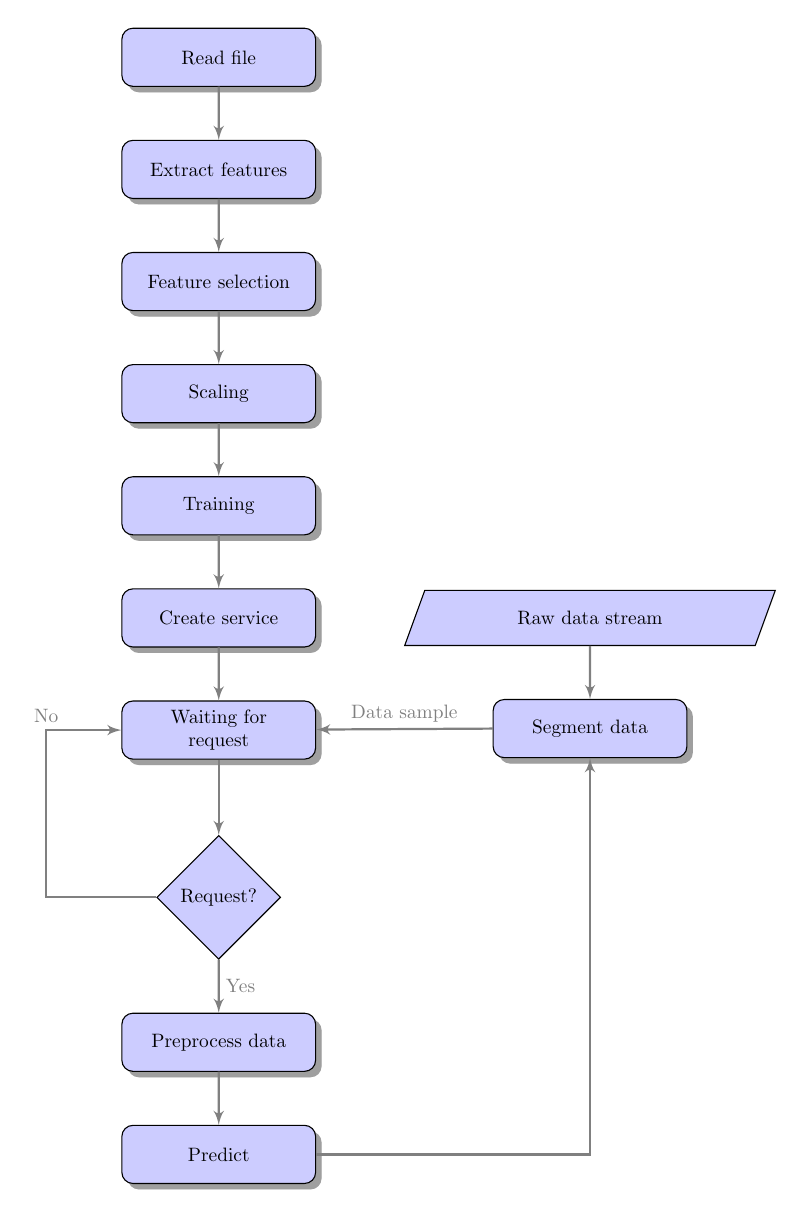
\begin{tikzpicture}[scale=0.7,transform shape]
		
		% Draw diagram elements
		%  \path \io{1}{Raw data};
		\path \etape{1}{Read file};
		%  \path (p1.south)+(0,-1.5) \etape{2}{Extract steps};
		\path (p1.south)+(0.0,-1.5) \etape{2}{Extract features};
		\path (p2.south)+(0.0,-1.5) \etape{3}{Feature selection};
		
		\path (p3.south)+(0.0,-1.5) \etape{4}{Scaling};
		\path (p4.south)+(0.0,-1.5) \etape{12}{Training};
		
		\path (p12.south)+(0,-1.5) \etape{5}{Create service};
		\path (p5.south)+(0,-1.5) \etape{6}{Waiting for request};
		\path (p6.south)+(0,-2.5) \dec{7}{Request?};
		\path (p7.south)+(0,-1.5) \etape{8}{Preprocess data};
		\path (p8.south)+(0,-1.5) \etape{9}{Predict};
		
		
		%\path (request?.south)+(0,-1.5) \etape{7}{Predicted};
		
		\path (p5.west)+(8.5,0) \io{10}{Raw data stream};
		\path (p10.south)+(0,-1.5) \etape{11}{Segment data};
		
		
		
		
		
		% Draw arrows between elements
		\path [line] (p1.south) -- node [above] {} (p2);
		\path [line] (p2.south) -- node [above] {} (p3);
		\path [line] (p3.south) -- node [above] {} (p4);
		\path [line] (p4.south) -- node [above] {} (p12);
		\path [line] (p12.south) -- node [above] {} (p5);
		\path [line] (p5.south) -- node [above] {} (p6);
		\path [line] (p6.south) -- node [above] {} (p7);
		\path [line] (p7.south) -- node [right] {Yes} (p8);
		\path [line] (p7.west) -- ++(-2,0) |- node [above] {No} (p6);
		\path [line] (p8.south) -- node [above] {} (p9);
		\path [line] (p9.east) -| node [above] {} (p11);
		
		\path [line] (p10.south) -- node [above] {} (p11);
		\path [line] (p11.west) -- node [above] {Data sample} (p6);
		\end{tikzpicture}
		
		\caption{Figure showing the real-time implementation} \label{fig:realtime}
	\end{figure}
	\FloatBarrier
	\clearpage

\subsection{Result and analysis} \label{sub:unseen}	
In following paragraphs present the results along with analysis of each experiments, when the robot traverse through two different terrains in this order:
	\begin{enumerate}
	\item Floor to carpet
	\item Hard mat to floor
	\item Hard mat to soft mat
	\item Soft mat to hard mat
	\item Soft mat to carpet
\end{enumerate}
\newpage

\subsubsection{Floor to carpet}
The data stream is shown in figure \ref{fig:gulvet4teppegraf}, where the dashed line is the transition between the terrains, and the table \ref{tab:Gulvet4teppe} show probability of the terrains for each step. In this experiment the robot walked four step on floor and the rest on carpet. The accuracy of predicting correct is 88.9\%. However, looking how certain the classifier to predict correct is lower, under 78\%. Fifth step is the transition and as it shows some confusion between floor and carpet. It is worth noticing that at fourth step the carpet has almost same probability as the floor. The soft mat and hard mat has small probability and is more unlikely to be predicted.
	
	\begin{figure}[h]
		\centering
		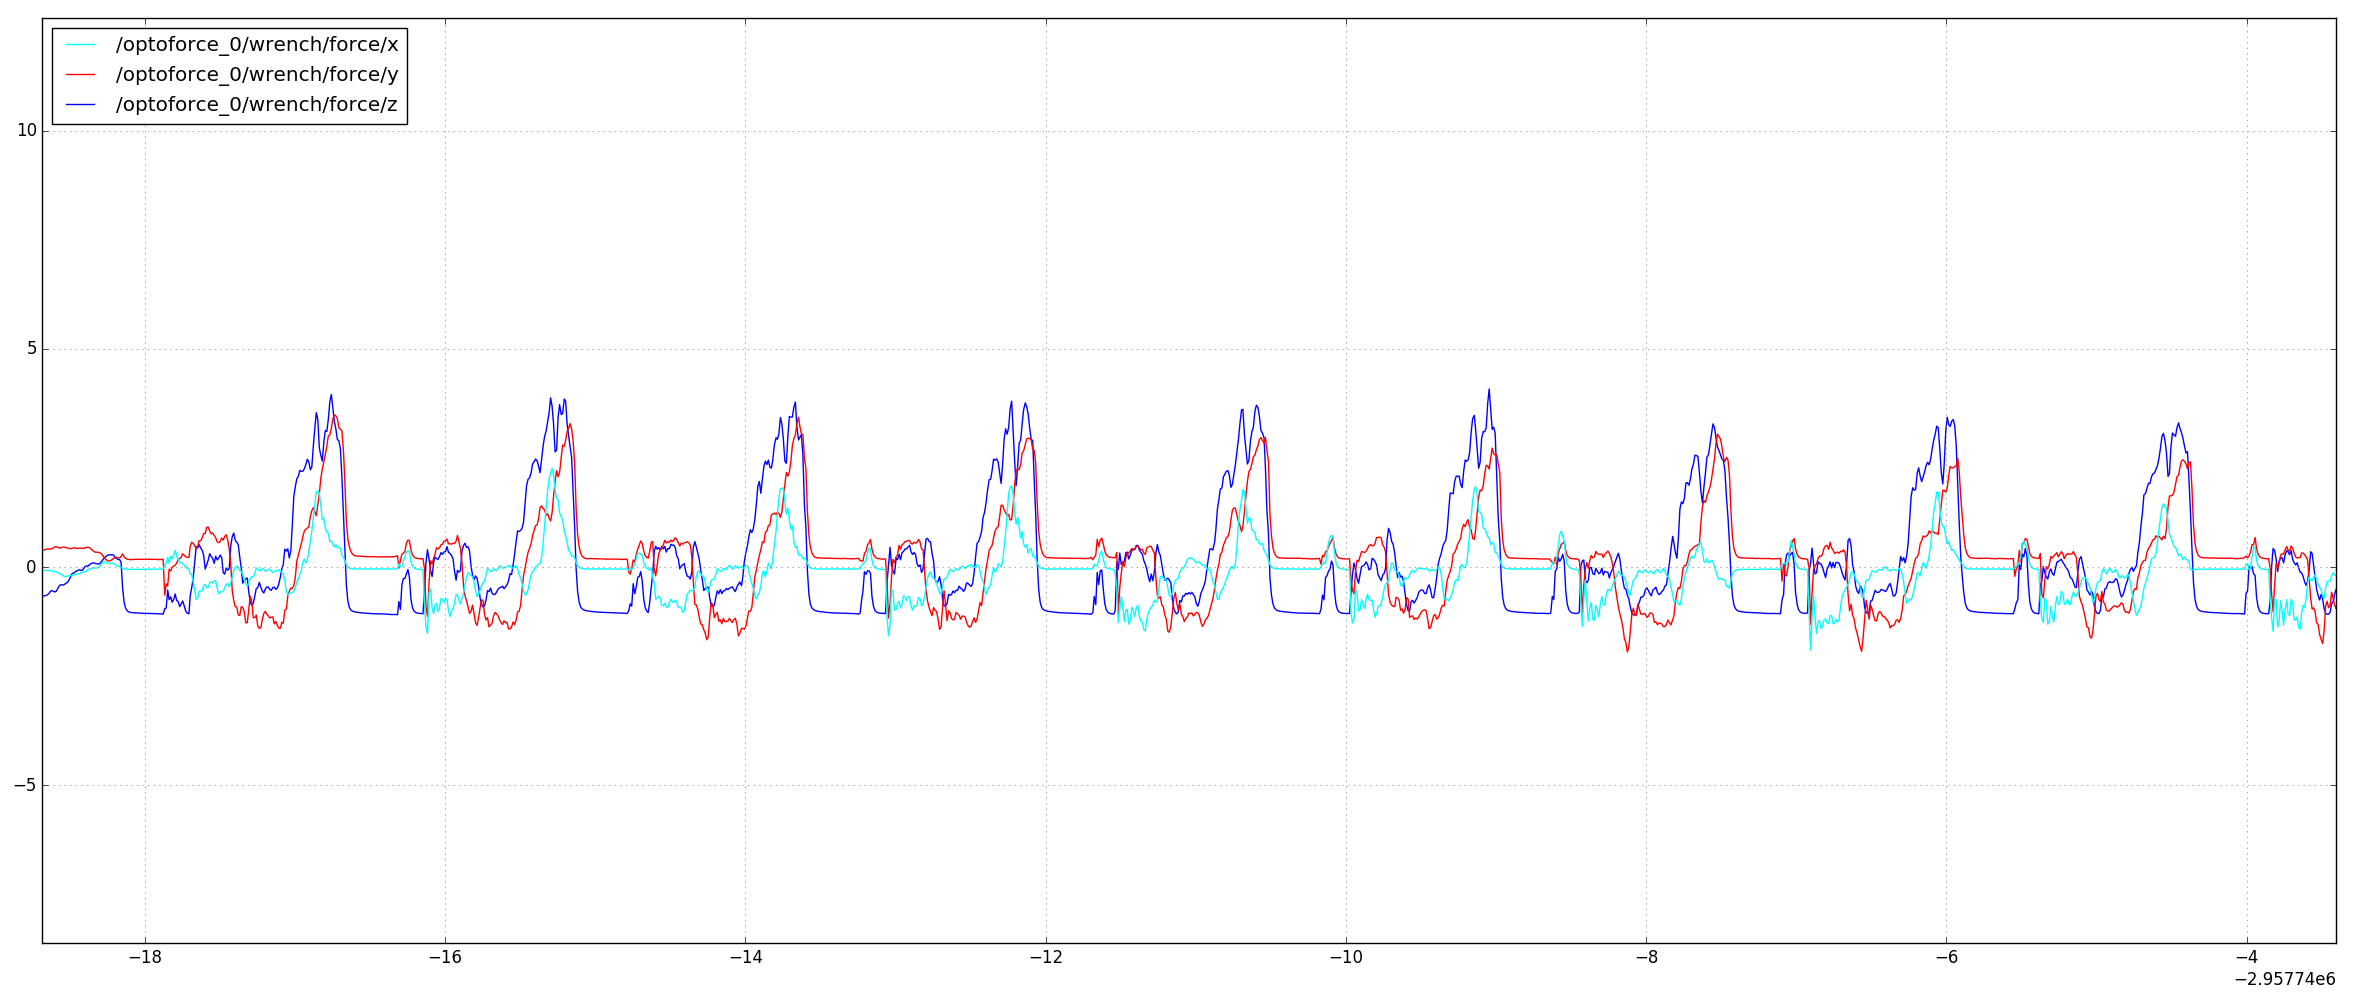
\includegraphics[width=\textwidth,height=\textheight,keepaspectratio]{Figures/Gulvet4Teppe2}
		\caption{Figure showing data stream from sensor when the robot walked from floor to carpet.}
		\label{fig:gulvet4teppegraf}
	\end{figure}
	
	
	\begin{table}[h]
		\centering
		\resizebox{\textwidth}{!}{%
			\begin{tabular}{@{}llllllllll@{}}
				\toprule
				\rowcolor[HTML]{FFFFC7} 
				\textbf{Step} & \textbf{1} & \textbf{2} & \textbf{3} & \textbf{4} & \textbf{5} & \textbf{6} & \textbf{7} & \textbf{8} & \textbf{9} \\ \midrule
				Floor & \cellcolor[HTML]{34FF34}0.782 & \cellcolor[HTML]{34FF34}0.680 & \cellcolor[HTML]{34FF34}0.747 & \cellcolor[HTML]{34FF34}0.561 & \cellcolor[HTML]{FD6864}0.564 & 0.282 & 0.206 & 0.252 & 0.282 \\
				Carpet & 0.105 & 0.289 & 0.162 & 0.425 & \cellcolor[HTML]{F8FF00}0.353 & \cellcolor[HTML]{34FF34}0.704 & \cellcolor[HTML]{34FF34}0.730 & \cellcolor[HTML]{34FF34}0.573 & \cellcolor[HTML]{34FF34}0.599 \\
				Soft mat & 0.008 & 0.009 & 0.010 & 0.008 & 0.010 & 0.005 & 0.009 & 0.009 & 0.015 \\
				Hard mat & 0.104 & 0.022 & 0.081 & 0.007 & 0.073 & 0.010 & 0.055 & 0.166 & 0.104 \\ \bottomrule
			\end{tabular}%
		}
		\caption{The table showing probability of each terrain per step from floor to carpet. Marked green represent correct prediction and correct terrain, red represent wrong prediction and yellow is the correct prediction if it got wrong.}
		\label{tab:Gulvet4teppe}
	\end{table}
	\FloatBarrier
	
	\clearpage
\subsubsection{Hard mat to floor} \label{subsec:hmf}
The data is shown in figure \ref{fig:mb3Gulvet} and the table \ref{tab:mb3Gulvet} show how the probability of each step, walking from hard mat to floor. The overall accuracy of predicting correct is 50\%. It can be seen that the first two step it is clearly what terrain it is on. While the third step start to be confused between hard mat and carpet. When it is on floor it rather predicting the floor.
	
	
	
	\begin{figure}[h]
		\centering
		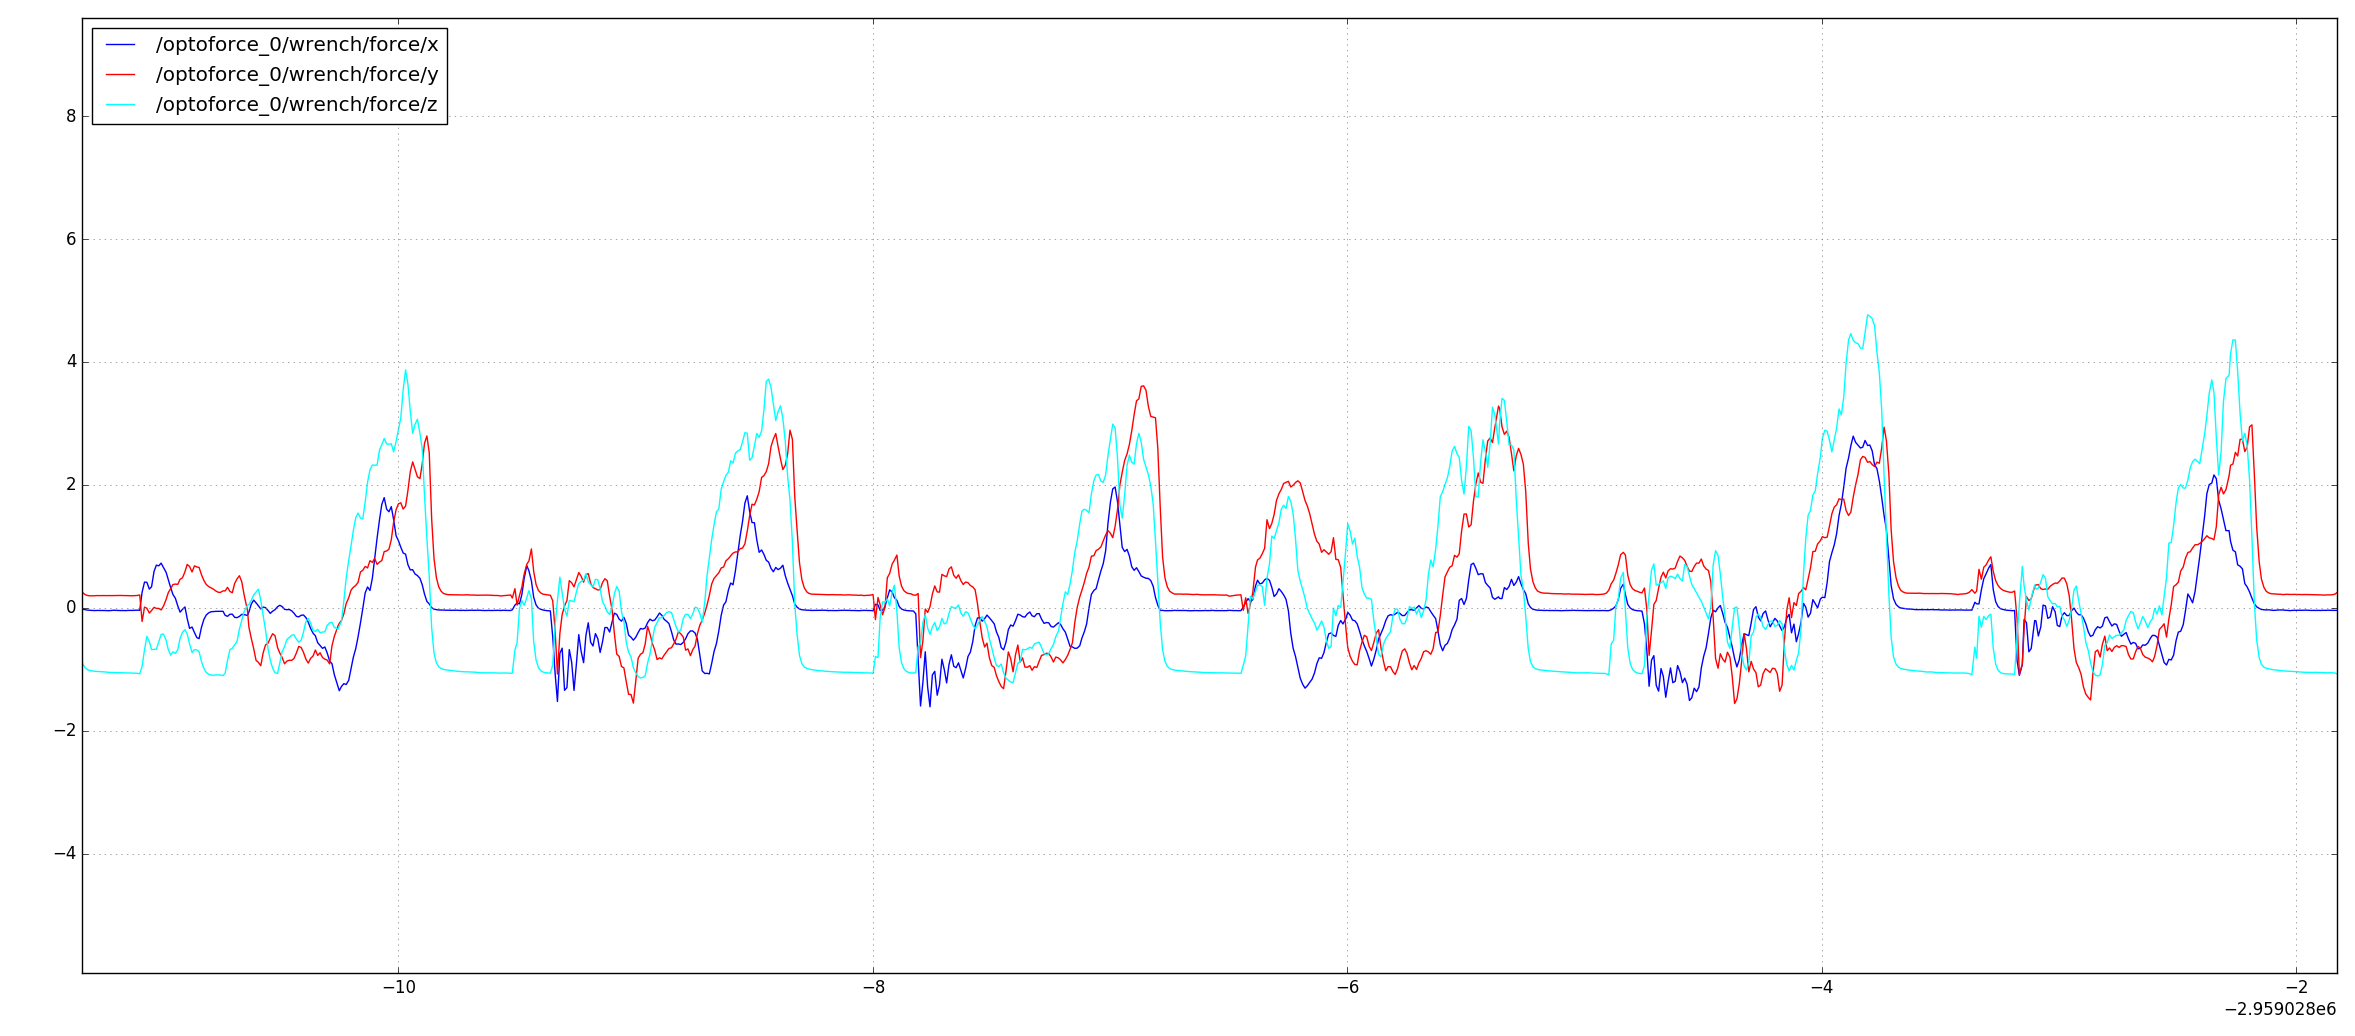
\includegraphics[width=\textwidth,height=\textheight,keepaspectratio]{Figures/MB3_3_Gulvet}
		\caption{Figure showing data stream from sensor when the robot walked from hard mat to floor}
		\label{fig:mb3Gulvet}
	\end{figure}
	
	
	\begin{table}[h]
		\centering
		\resizebox{\textwidth}{!}{%
			\begin{tabular}{@{}lllllll@{}}
				\toprule
				\rowcolor[HTML]{FFFFC7} 
				\textbf{Step} & \textbf{1} & \textbf{2} & \textbf{3} & \textbf{4} & \textbf{5} & \textbf{6} \\ \midrule
				Floor & 0.006 & 0.008 & 0.172 & \cellcolor[HTML]{F8FF00}0.263 & \cellcolor[HTML]{F8FF00}0.141 & \cellcolor[HTML]{F8FF00}0.078 \\
				Carpet & 0.008 & 0.073 & 0.375 & \cellcolor[HTML]{FD6864}0.641 & \cellcolor[HTML]{FD6864}0.615 & \cellcolor[HTML]{FD6864}0.822 \\
				Soft mat & 0.006 & 0.004 & 0.008 & 0.023 & 0.019 & 0.014 \\
				Hard mat & \cellcolor[HTML]{34FF34}0.980 & \cellcolor[HTML]{34FF34}0.915 & \cellcolor[HTML]{34FF34}0.444 & 0.073 & 0.225 & 0.085 \\ \bottomrule
			\end{tabular}%
		}
		\caption{The table showing probability of each terrain per step walking from hard mat to floor. Marked green represent correct prediction and correct terrain, red represent wrong prediction and yellow is the correct prediction if it got wrong.}
		\label{tab:mb3Gulvet}
	\end{table}
	
	\FloatBarrier
	\clearpage
\subsubsection{Hard mat to soft mat} \label{sec:hmssm}
The data is shown in figure \ref{fig:hardmatSoftMat} and the table \ref{hardmatSoftMat} show how the probability of each step in transition from hard mat to soft mat. As seen on the figure \ref{fig:hardmatSoftMat} there is a clearly difference between walking on hard mat and soft mat. Hard mat has a higher force in every direction. However, there are some uncertain of prediction on the first, third and sixth step, where it has a probability under 54\%. 
	
	
	\begin{figure}[h]
		\centering
		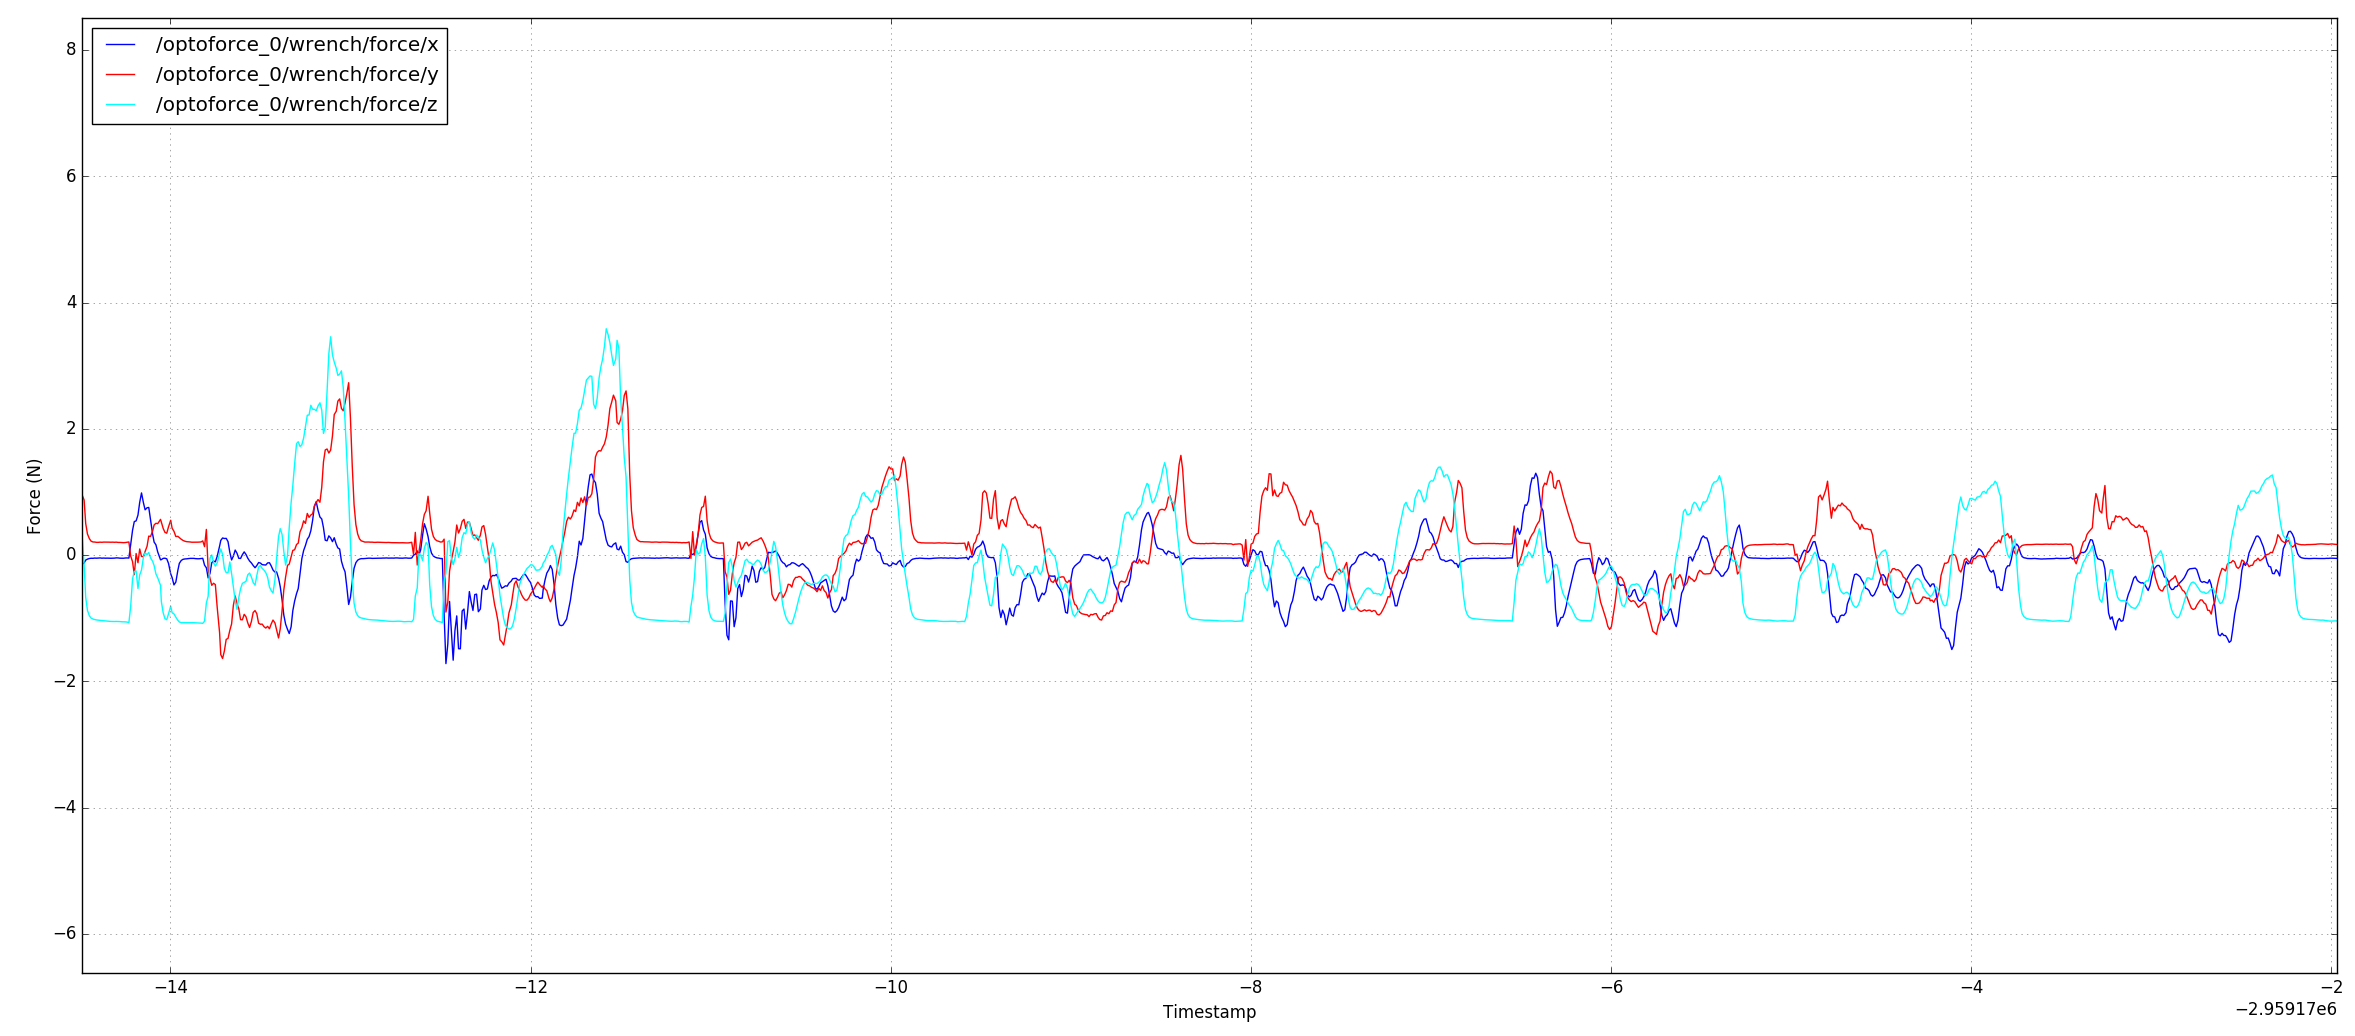
\includegraphics[width=\textwidth,height=\textheight,keepaspectratio]{Figures/MB3MM}
		\caption{Figure showing data stream from sensor when the robot walked from hard mat to soft mat.}
		\label{fig:hardmatSoftMat}
	\end{figure}
	
	\begin{table}[h]
		\centering
		\resizebox{\textwidth}{!}{%
			\begin{tabular}{@{}lllllllll@{}}
				\toprule
				\rowcolor[HTML]{FFFFC7} 
				\textbf{Step} & \textbf{1} & \textbf{2} & \textbf{3} & \textbf{4} & \textbf{5} & \textbf{6} & 7 & 8 \\ \midrule
				Floor & 0.329 & 0.015 & 0.081 & 0.059 & 0.022 & 0.115 & 0.059 & 0.048 \\
				Carpet & 0.105 & 0.045 & 0.105 & 0.041 & 0.015 & 0.095 & 0.037 & 0.033 \\
				Soft mat & 0.023 & 0.006 & 0.284 & \cellcolor[HTML]{34FF34}0.759 & \cellcolor[HTML]{34FF34}0.923 & \cellcolor[HTML]{34FF34}0.477 & \cellcolor[HTML]{34FF34}0.816 & \cellcolor[HTML]{34FF34}0.834 \\
				Hard mat & \cellcolor[HTML]{34FF34}0.542 & \cellcolor[HTML]{34FF34}0.935 & \cellcolor[HTML]{34FF34}0.529 & 0.142 & 0.040 & 0.313 & 0.088 & 0.085 \\ \bottomrule
			\end{tabular}%
		}
		\caption{The table showing probability of each terrain per step walking from hard mat to soft mat. Marked green represent correct prediction and correct terrain, red represent wrong prediction and yellow is the correct prediction if it got wrong.}
		\label{hardmatSoftMat}
	\end{table}
	\FloatBarrier
	\clearpage
	
\subsubsection{Soft mat to hard mat}
The data stream is shown in figure \ref{fig:MM_4_Resten_BGraf} and the table \ref{MM4MB} show probability of the terrains for each step. Again, the accuracy of predicting correct is 100\%. In this experiment the classifier is able without any problem. However prediction at beginning (first step), and the step right before new terrain (fourth step), has probability under 53\%.
	
	\begin{figure}[h]
		\centering
		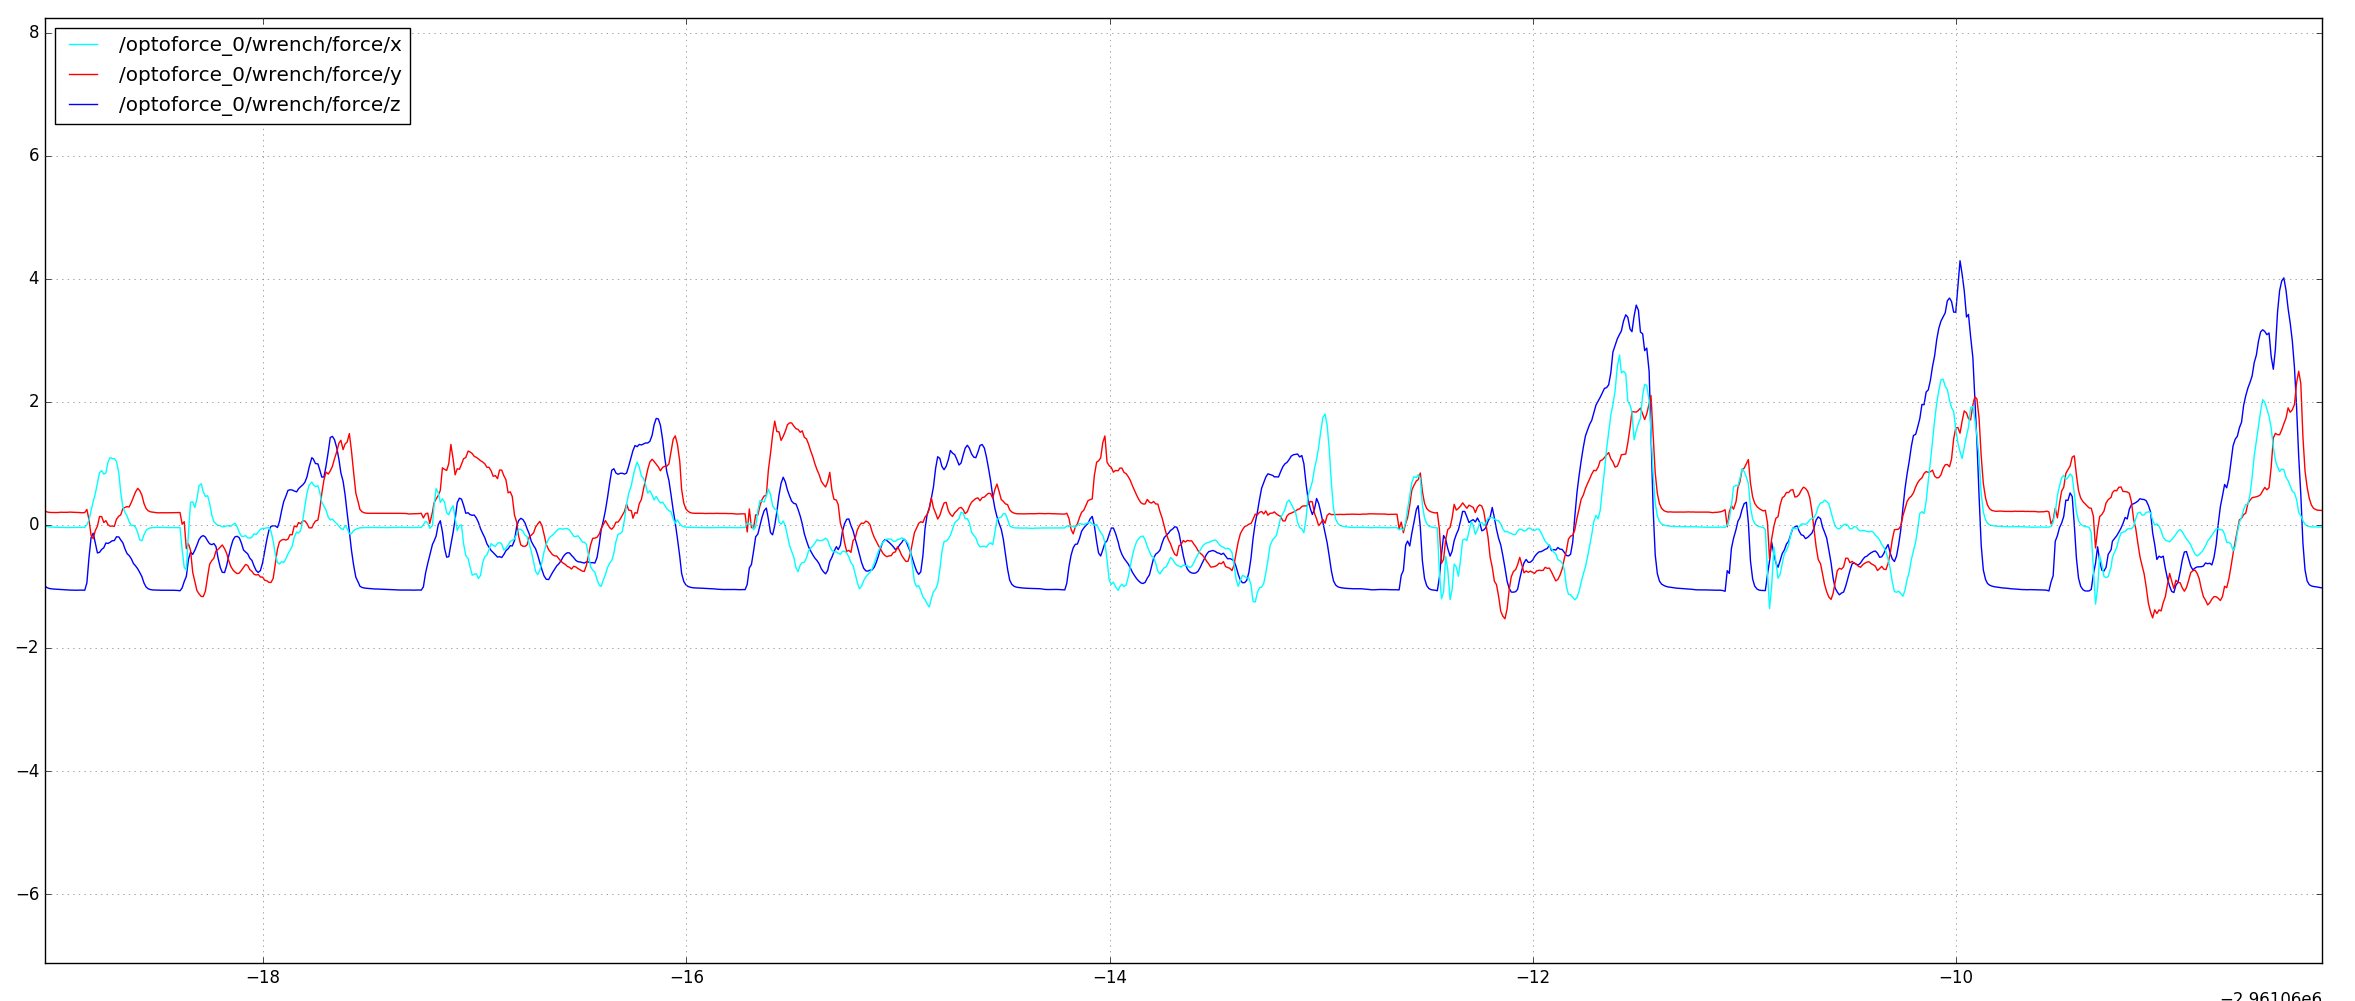
\includegraphics[width=\textwidth,height=\textheight,keepaspectratio]{Figures/MM_4Resten_MB}
		\caption{Figure showing data stream from sensor when the robot walked from soft mat to hard mat.}
		\label{fig:MM_4_Resten_BGraf}
	\end{figure}
	
	\begin{table}[h]
		\centering
		\resizebox{\textwidth}{!}{%
			\begin{tabular}{@{}llllllll@{}}
				\toprule
				\rowcolor[HTML]{FFFFC7} 
				\textbf{Step} & \textbf{1} & \textbf{2} & \textbf{3} & \textbf{4} & \textbf{5} & \textbf{6} & 7 \\ \midrule
				Floor & 0.099 & 0.019 & 0.018 & 0.138 & 0.021 & 0.008 & 0.038 \\
				Carpet & 0.065 & 0.023 & 0.017 & 0.134 & 0.050 & 0.005 & 0.022 \\
				Soft mat & \cellcolor[HTML]{34FF34}0.535 & \cellcolor[HTML]{34FF34}0.871 & \cellcolor[HTML]{34FF34}0.911 & \cellcolor[HTML]{34FF34}0.384 & 0.009 & 0.009 & 0.011 \\
				Hard mat & 0.300 & 0.086 & 0.054 & 0.344 & \cellcolor[HTML]{34FF34}0.921 & \cellcolor[HTML]{34FF34}0.978 & \cellcolor[HTML]{34FF34}0.930 \\ \bottomrule
			\end{tabular}%
		}
		\caption{The table showing probability of each terrain per step walking from soft mat to hard mat. Marked green represent correct prediction and correct terrain, red represent wrong prediction and yellow is the correct prediction if it got wrong.}
		\label{MM4MB}
	\end{table}
	\FloatBarrier
	\clearpage
\subsubsection{Soft mat to carpet}
The data stream is shown in figure \ref{fig:softcarpet} and the table \ref{tab:softcarpet} show probability of the terrains for each step. It has predicted 7 of 8 correctly. As seen in the figure \ref{fig:softcarpet}, there is a large variation from walking soft mat to carpet. On small soft mat the amplitude is significant smaller than carpet. At the fifth step is when the robot walked from the old terrain to the new one, and the probability of carpet is approximately 66.7\%. However the second highest has a probability of 21.6\%, which it clear what terrain it is. Regarding sixth step, the classifier has a wrong prediction between carpet and hard mat. There is a high probability of hard hard mat.
	
	
	
	\begin{figure}[h]
		\centering
		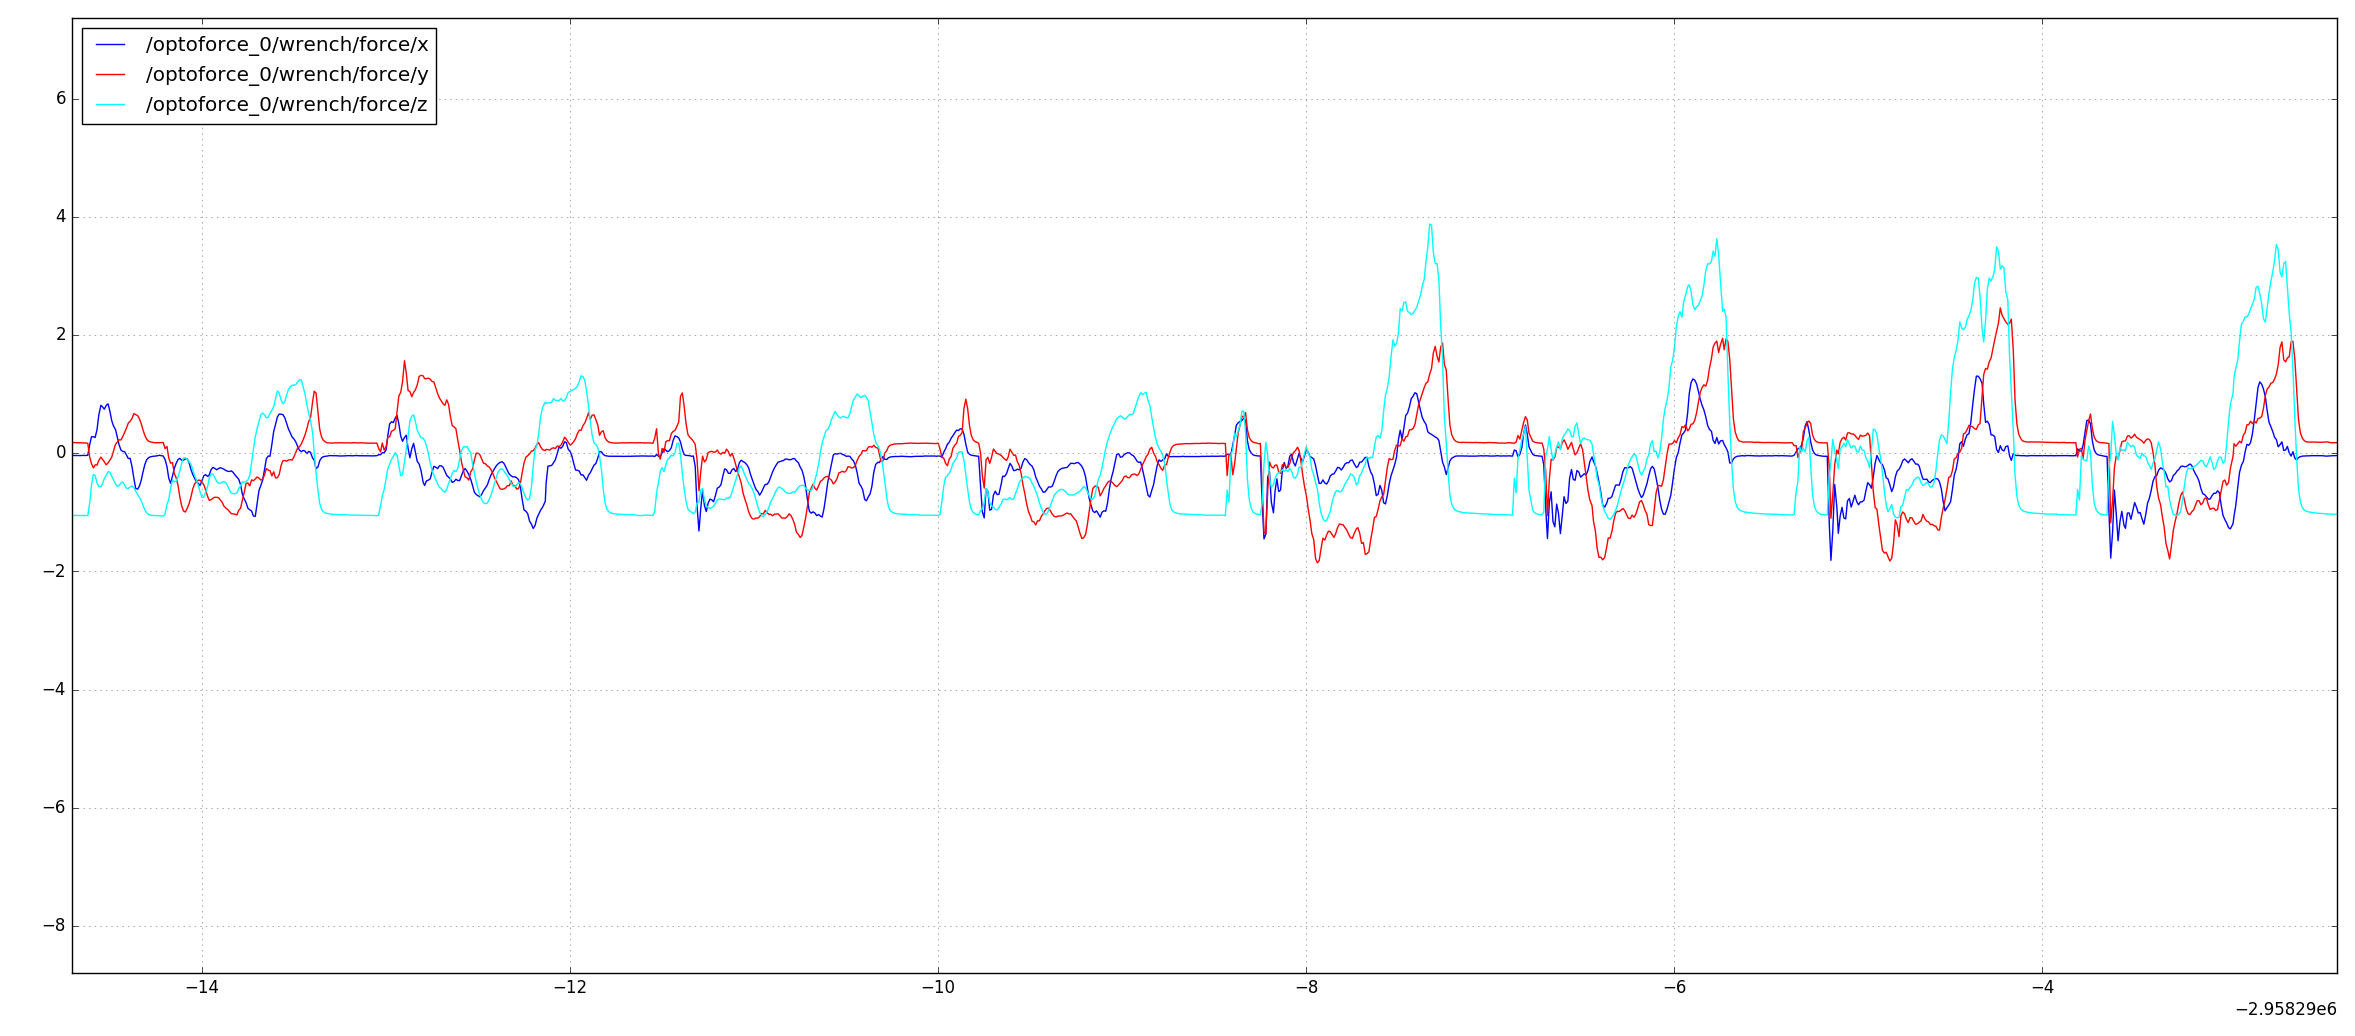
\includegraphics[width=\textwidth,height=\textheight,keepaspectratio]{Figures/MM4Teppe2}
		\caption{Figure showing data stream from sensor when the robot walked from soft mat to carpet.}
		\label{fig:softcarpet}
	\end{figure}
	
	\begin{table}[h]
		\centering
		\resizebox{\textwidth}{!}{%
			\begin{tabular}{@{}lllllllll@{}}
				\toprule
				\rowcolor[HTML]{FFFFC7} 
				\textbf{Step} & \textbf{1} & \textbf{2} & \textbf{3} & \textbf{4} & \textbf{5} & \textbf{6} & 7 & 8 \\ \midrule
				Floor & 0.021 & 0.022 & 0.068 & 0.031 & 0.100 & 0.020 & 0.016 & 0.018 \\
				Carpet & 0.017 & 0.019 & 0.049 & 0.023 & \cellcolor[HTML]{34FF34}0.667 & \cellcolor[HTML]{F8FF00}0.041 & \cellcolor[HTML]{34FF34}0.942 & \cellcolor[HTML]{34FF34}0.904 \\
				Soft mat & \cellcolor[HTML]{34FF34}0.909 & \cellcolor[HTML]{34FF34}0.914 & \cellcolor[HTML]{34FF34}0.762 & \cellcolor[HTML]{34FF34}0.891 & 0.017 & 0.007 & 0.006 & 0.006 \\
				Hard mat & 0.054 & 0.045 & 0.121 & 0.055 & 0.216 & \cellcolor[HTML]{FD6864}0.933 & 0.037 & 0.072 \\ \bottomrule
			\end{tabular}%
		}
		\caption{The table showing probability of each terrain per step walking from soft mat to carpet. Marked green represent correct prediction and correct terrain, red represent wrong prediction and yellow is the correct prediction if it got wrong.}
		\label{tab:softcarpet}
	\end{table}
	\FloatBarrier
\newpage

\subsection{Summary}
In this experiment, five different transition between two terrains were tested. A common characteristic is that the probability decreases particular on the transition step. It predicts correct when the terrain has a huge difference to the other such as soft mat, while transition between more similar terrain has a wrong prediction at the transition. The first step has a tendency to either have relative high probability approximately 90\%, or low probability approximately 54\%.
	
	
\section{Prediction on other sensor}
The classification has been based on only one sensor on front left foot, thus it will be interesting to see whether it is possible to use the currently training set to classify accurately on front right foot. Reason for testing the right front right foot, is because it has more similar motion to the left front foot. The back foot on other hand, has a different leg motion which provide a different data in each direction. Thus in following experiment will be collecting 30 data samples right foot for each terrain. A reason for this experiments is if it achieve a high accuracy might indicate that one the both feet on the front can be using the same training set instead of separately which is more convenient.

	
\subsection{Results} 
The table \ref{tab:pred} shows the result of prediction of the other sensor.
\begin{table}[h]
	\centering
	\begin{tabular}{lllll}
		\hline
		\textbf{Terrain} & \textbf{Floor} & \textbf{Carpet} & \textbf{Soft mat} & \textbf{Hard mat} \\ \hline
		\textbf{Floor} & \cellcolor[HTML]{FFFFC7}29 & 1 & 0 & 0 \\
		\textbf{Carpet} & 3 & \cellcolor[HTML]{FFFFC7}27 & 0 & 0 \\
		\textbf{Soft mat} & 0 & 0 & \cellcolor[HTML]{FFFFC7}30 & 0 \\
		\textbf{Hard mat} & 2 & 13 & 0 & \cellcolor[HTML]{FFFFC7}16 \\ \hline
		\textbf{Precision} & 96.7\% & 90\% & 100\% & 53.3\% \\
		\textbf{Recall} & 85.3\% & 65.9\% & 100\% & 100\% \\
		\textbf{F-score} & 90.6\% & 76.1\% & 100\% & 69.5\% \\ \hline
		\textbf{Accuracy} & \multicolumn{4}{c}{84.3\%} \\ \hline
	\end{tabular}
	\caption{Table shows metrics of predicting on other sensor.}
	\label{tab:pred}
\end{table}
	\FloatBarrier
	
\subsection{Analysis} 	
The overall accuracy of predicting on the other sensor is 84.3\% as seen in table \ref{tab:pred}. It is precise to predict floor, carpet, and soft mat with precision of at leas 90\%. It also show similar confusion as previous experiments in section \ref{sub:unseen}, when it has a tendency to predict hard mat as carpet.
\\
\\
It will be interesting to see the data provided from each sensor, which is shown in figure \ref{fig:s1all}. Forces in z-direction is almost same for floor,carpet, and hard mat, but a big difference with the soft mat. 

\begin{figure} [h]
	\centering
	\begin{subfigure}[b]{\textwidth}
			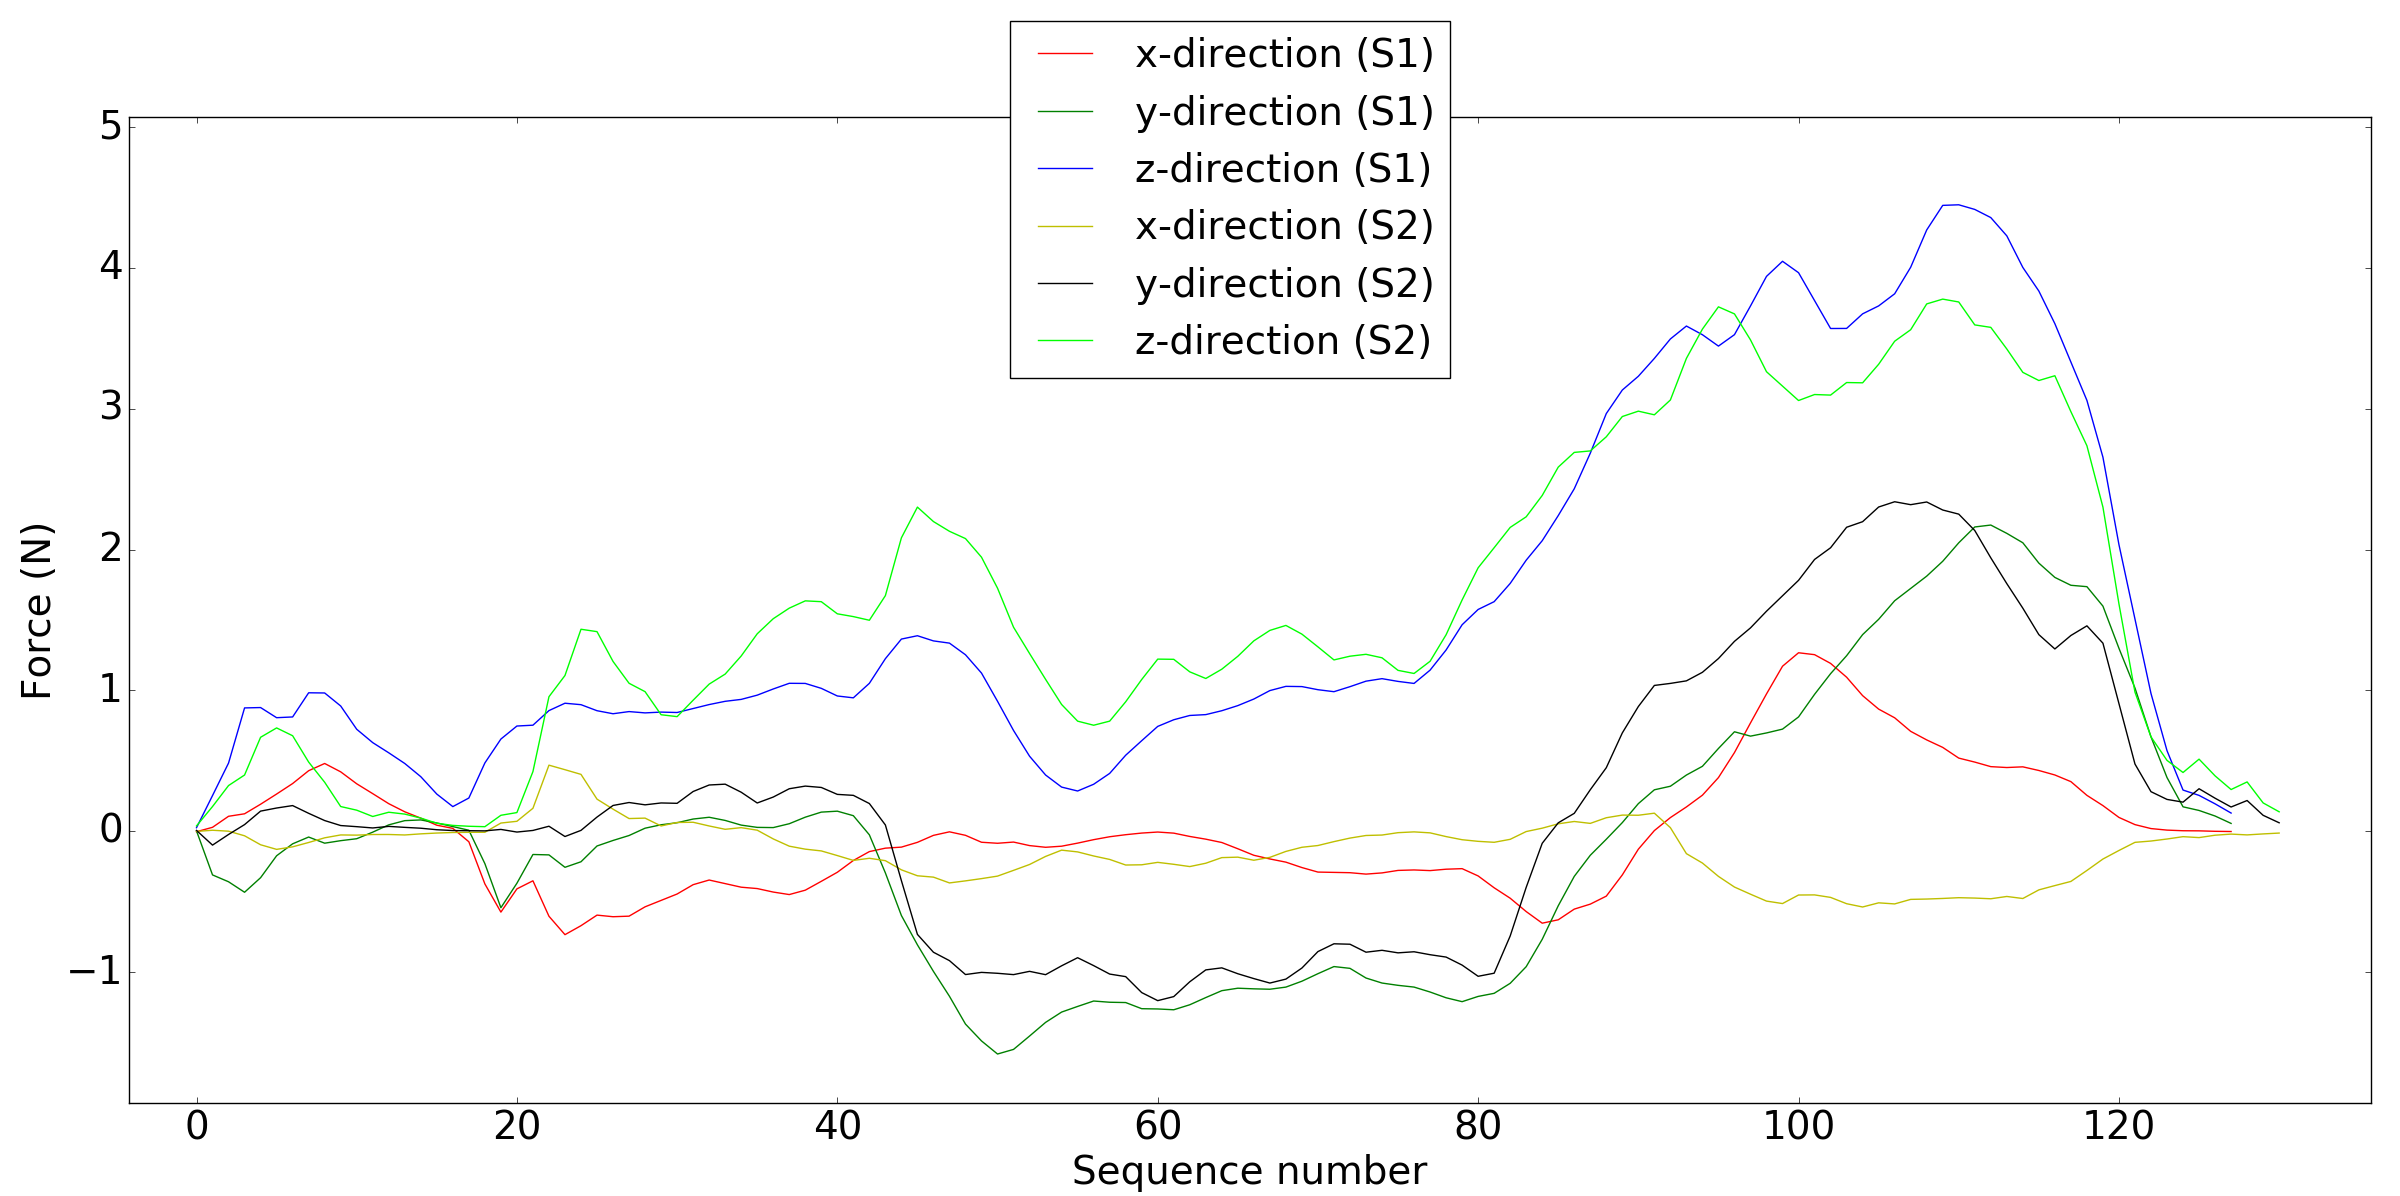
\includegraphics[width=\textwidth,height=\textheight,keepaspectratio]{Figures/s1gulv2}
			\caption{Floor}
			\label{fig:s1gulv2} 
		\end{subfigure}
		
		\begin{subfigure}[b]{\textwidth}
			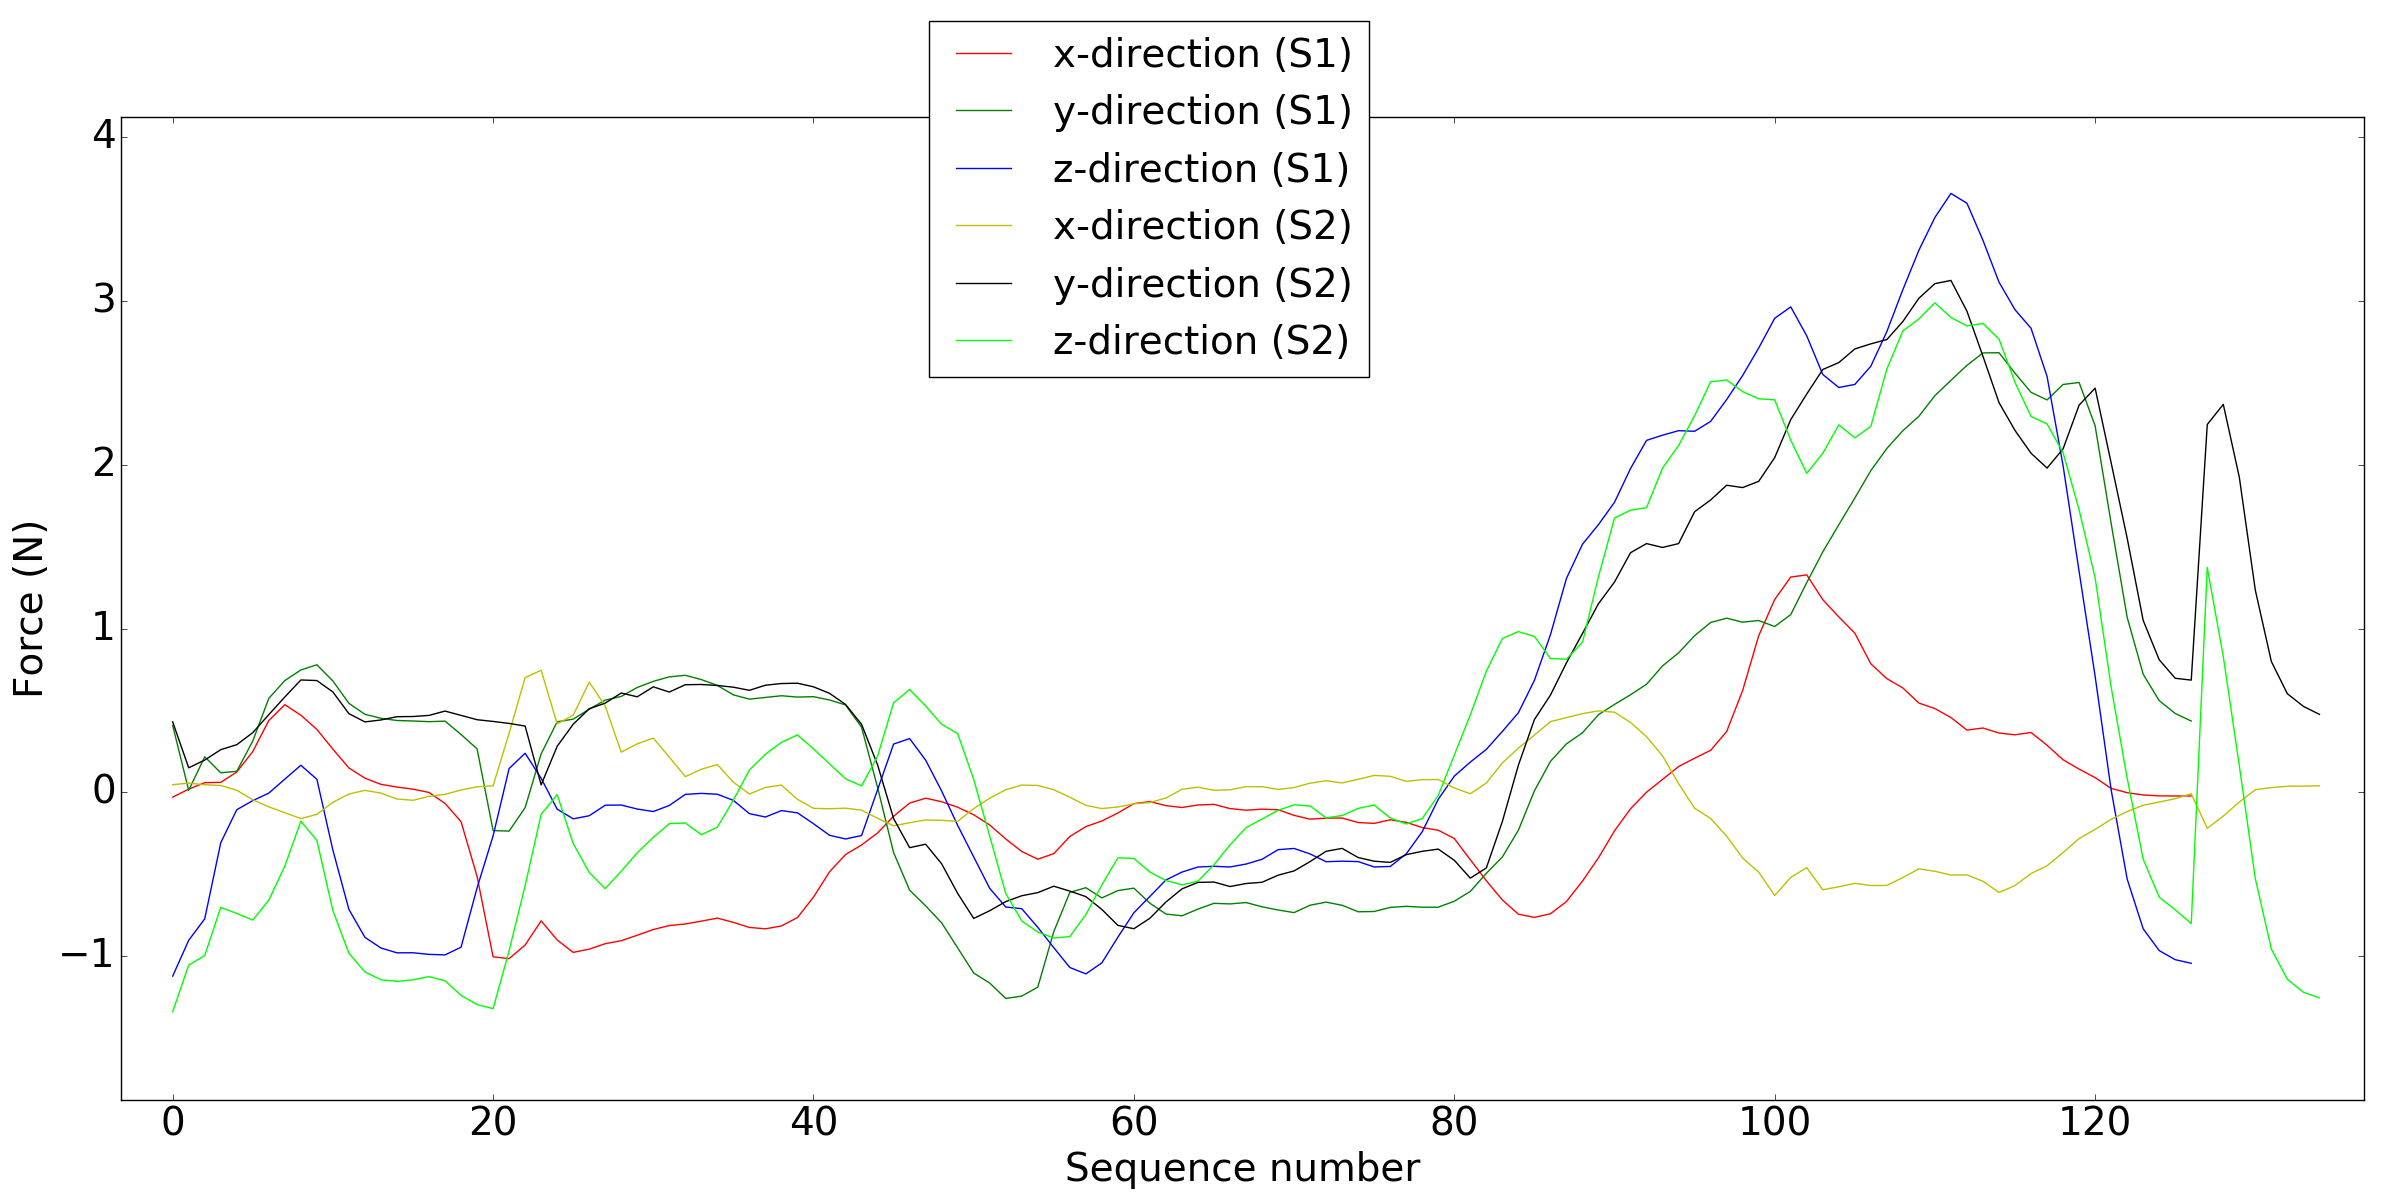
\includegraphics[width=\textwidth,height=\textheight,keepaspectratio]{Figures/s1teppe}
			\caption{Carpet}
			\label{fig:s1teppe}
		\end{subfigure}
		
	\end{figure}
	\begin{figure}[h] \ContinuedFloat
		\begin{subfigure}[h]{\textwidth}
			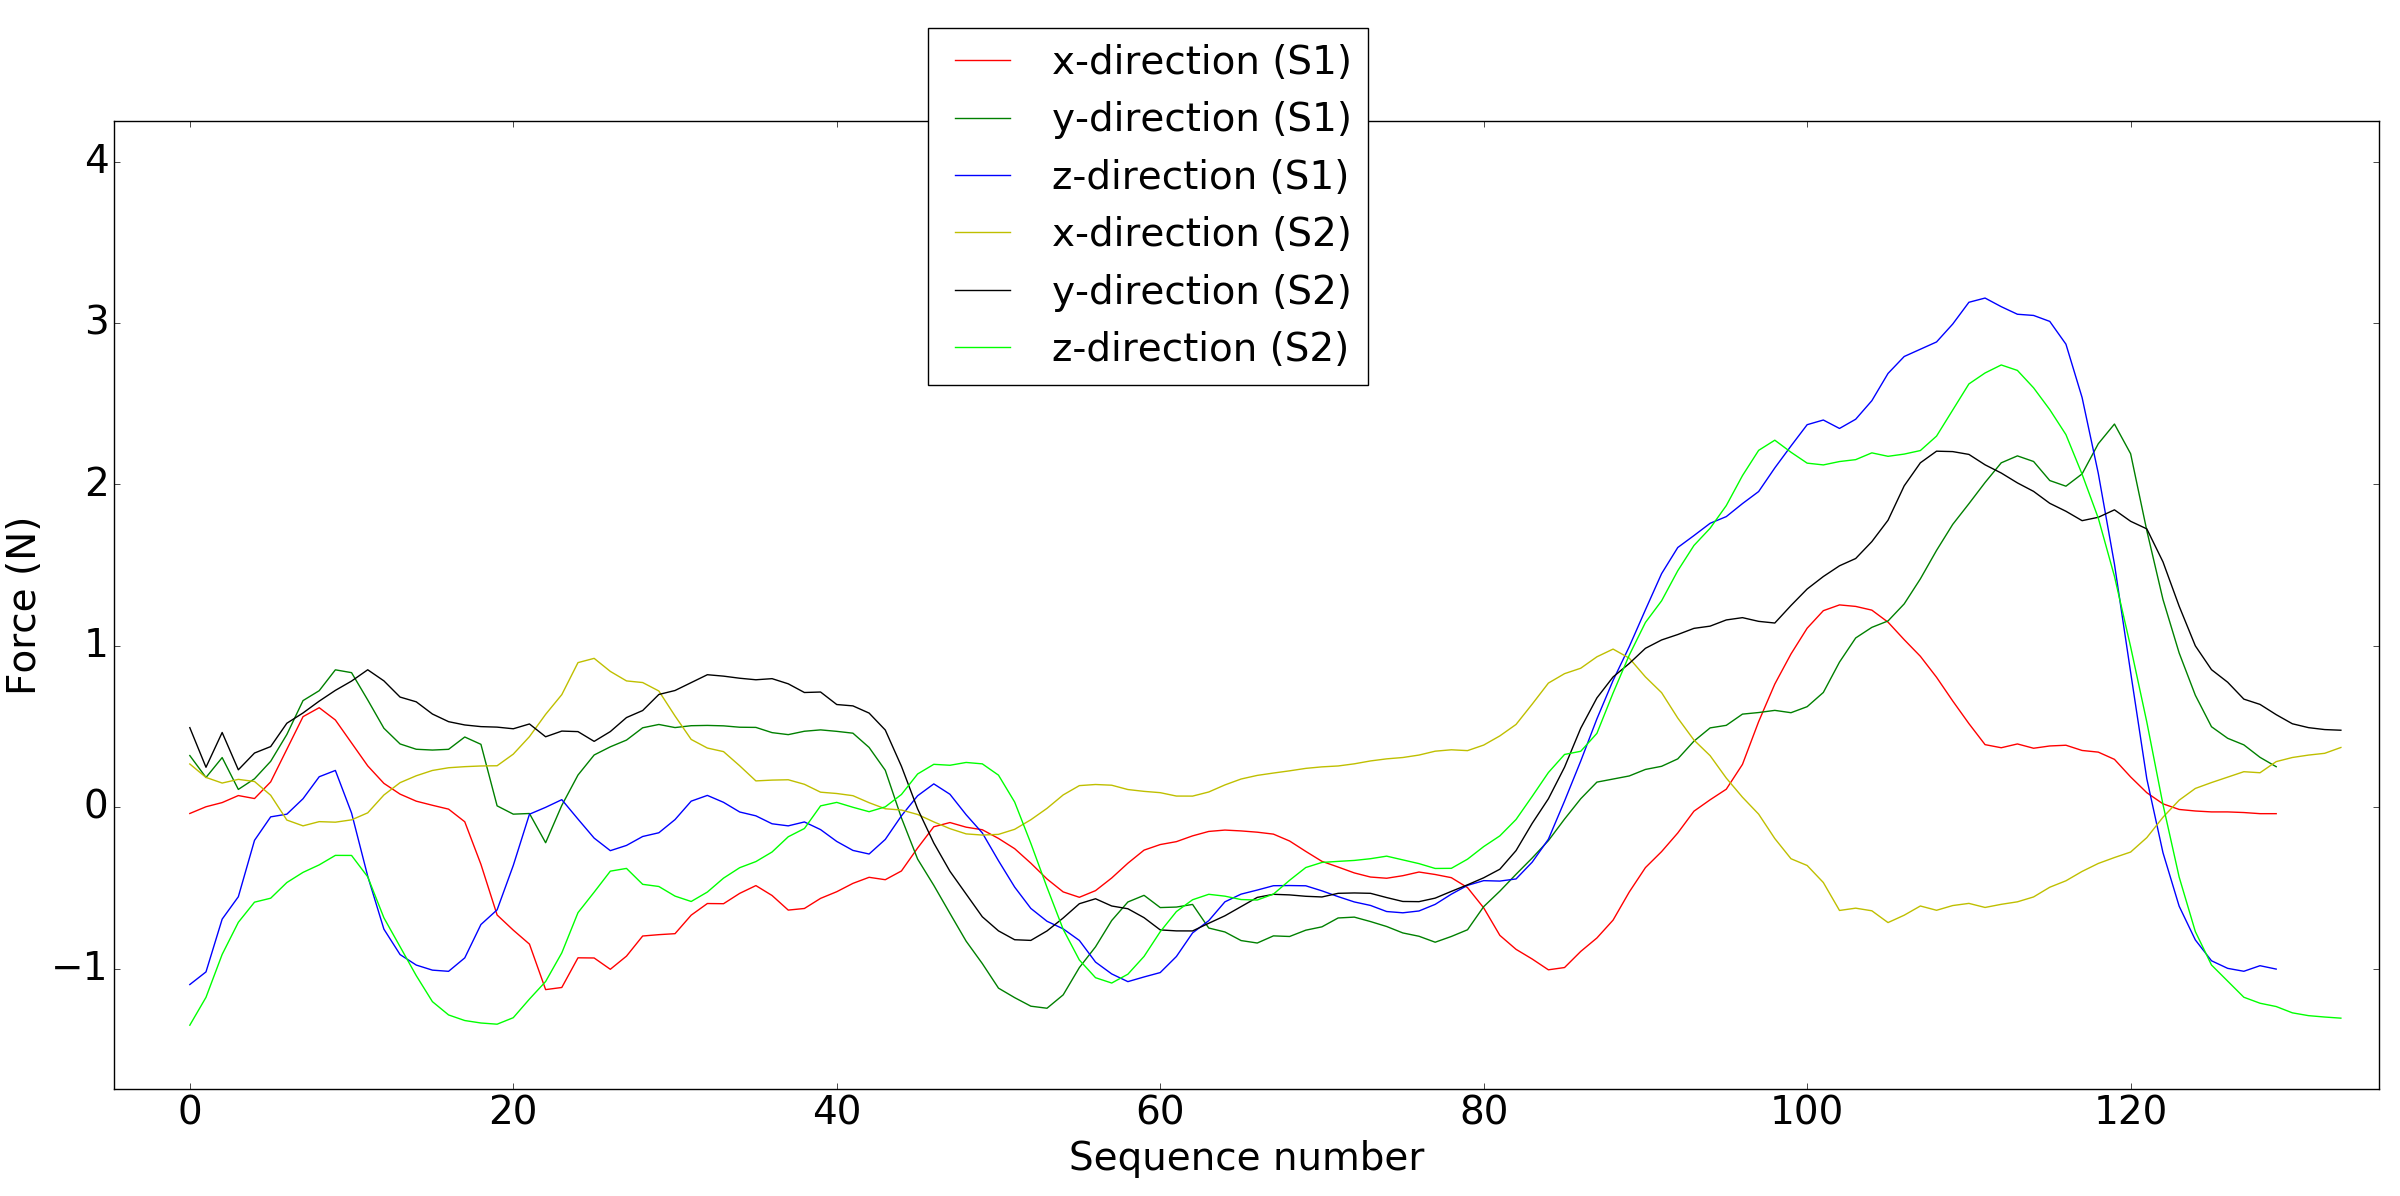
\includegraphics[width=\textwidth,height=\textheight,keepaspectratio]{Figures/s1hardmatte}
			\caption{Hard mat}
			\label{fig:s1hardmatte}
		\end{subfigure}
		\begin{subfigure}[b]{\textwidth}
			\includegraphics[width=\textwidth,height=\textheight,keepaspectratio]{Figures/s1mykmatte}
			\caption{Soft mat}
			\label{fig:s1mykmatte}
		\end{subfigure}
		\caption[]{Figure showing data stream for each terrain in time. (a) floor (b) carpet (c) hard mat (d) soft mat }
		\label{fig:s1all}
	\end{figure}	
	\FloatBarrier



\chapter{Discussion}

\section{Five classifier prediction on unseen data}
It is shown that the many classifiers has decreased performance when it come to predicting unseen data. As seen in section \ref{seq:crossunseen}, the neural network and decision tree does not show adequate performance. A reason could be that the classifier is overfitted and not able to generalize the data. Note that those classifiers of raw data sequences, and the method of achieving fixed length by decimate data described in section \ref{subseq:FixLength} might been affecting the performance. In this approach it is considered that data at start and the end of sequence is less important. However, the longer the sequence is, the more data must be removed from the feature vector and has a risk of removing important features. Another weakness of using raw data is the risk of learning with noises. Learning with noises might cause of not generalization the model and achieve a poor performance. However, noises are inherent in real world measurement, thus by discarding the noises might also give a poor result. Note each classifier use their default values which also affect the performance, especially neural network. The neural network is a complex classifier with many parameter that need to be adjusted such as size of hidden layers. Amount of hidden layers and hidden nodes provide significant improvement in their performance.  
\\
\\
Regarding a common confusion on hard mat, for each of classifier tend to predict it as carpet, while the soft mat has a high probability. As seen on previous chapter \ref{ch:implementation} in figures \ref{fig:meanxyz} and \ref{fig:fftxyz}, the hard mat and carpet has the most similar characteristic and is most likely to be confused.
\\
\\
Regarding SVM, the results has not been change during each run. That indicate the good features is kept and able to distinguish between each terrain. However, there is still a small confusion between floor, carpet and hard mat. 
	
\section{Hyperparameter-tuning}
The achieved parameters from grid search did not show a big effect on the performance. However, for the Neural Network it was only searching for number of neurons in one or two hidden layers, while there are many other settings which also should be tested to achieve a more optimal classifier. Regarding the number output, it can be seen the misclassification increase. Classification will be by considered of which neurons fire. However, when two neurons fires, the output will be an unknown, which cause misclassification. Two outputs on other hand, did have a minor improvement. Some of the reason there is a two output which have their weighted adjusted instead of having one input. Having two outputs where each of terrain is represent as binary number, the pattern of firing neurons will always belong to one of the terrains, even it one of the neurons misfiring. Minor improvement could be that a output with of two node has more weight to be adjusted which also 

\section{Transition between terrains}
The result achieved in transition between terrains, done in section \ref{sec:realtime}, indicates that the classifier is able to identify terrains even with minor differences in their properties. By adding each step and divide by total, the overall accuracy is  86.8\%. Misclassification is mostly cause of transition between hard mat to floor, seen in table \ref{sec:hmssm}. After traversing from hard mat to carpet, the classifier tend to predict floor. Looking on estimation of unseen data in table \ref{svmexp}, show a that the carpet tend to have small misclassification to floor. But, as mentioned in section \ref{sec:realtime}, the robot tend to not walking straight, which might cause misclassification. All of the training samples has been gathered when the robot walked straight. Thus, since the sensor is highly sensitive it might be affected when it walks toward right or left.
\\
\\
Having training samples where the robot traversing straight through each of one terrain have shown some significant appreciable in their performance. Observations on steps before crossing to new terrain has a less probability of predicting correct. A feasible method to prevent this, is to have training samples where it traverse through different terrains. However, misclassifying terrain when it cross should not be important when it is able to identify terrains after few step.    
\\
\\
Is also seen that in the beginning the probability of correct terrain is also typically low. It might indicate that the first step has a particular behavior, as the in the middle the robot got more stable, thus more training data on the first step to achieved higher probability on first step. It is shown that the sensor is capable to distinguish minor differently terrain, even the probability is low. Soft mat has a low start.
	
\subsection{Predicting on the other sensor}
It can be seen that the classifier had difficulty of predicting hard mat. As seen in the figures, the data provided from the right front foot differ some from the left front foot. However, there are characteristics such as shape and curve of the graphs. Note, the when mounting sensor on the foot there is a possibility of the sensor does not point on same directions. However, it mostly of the terrains have been predicted correct. The hard mat has been a common problem of the classifier. Beside of that, it is shown a possibility using the training data from the LF on RF.
	
\subsection{Compared to earlier work}
Looking of early similar approaches on table \ref{table:compareEarly}, the thesis approach has achieved reliable result by using the optical force sensor....  
	\begin{table}[h]
		\centering
		\resizebox{\textwidth}{!} \\
				&  &  &  &  \\
				&  &  &  &  \\
				\multirow{3}{*}{Kim el at. \cite{5602459}} & \multirow{3}{*}{\begin{tabular}[c]{@{}l@{}}Ground reaction force \\ Torque sensors\end{tabular}} & \multirow{3}{*}{SVM} & \multirow{3}{*}{4} & \multirow{3}{*}{78.75\%} \\
				&  &  &  &  \\
				&  &  &  &  \\
				\multirow{3}{*}{Kertész \cite{6849778}} & \multirow{3}{*}{\begin{tabular}[c]{@{}l@{}}Accelerometer\\ Paw sensor\end{tabular}} & \multirow{3}{*}{Naive Bayes} & \multirow{3}{*}{5} & \multirow{3}{*}{90.9\%} \\
				&  &  &  &  \\
				&  &  &  &  \\
				\multirow{2}{*}{Weiss el at. \cite{4059113}} & \multirow{2}{*}{Vibration} & \multirow{2}{*}{SVM} & \multirow{2}{*}{7} & \multirow{2}{*}{91.7\%} \\
				&  &  &  &  \\
				\multirow{2}{*}{Degrave el at. \cite{6784609}} & \multirow{2}{*}{Tactile sensor} & \multirow{2}{*}{Reservoir Computing} & \multirow{2}{*}{5} & \multirow{2}{*}{93.8\%} \\
				&  &  &  &  \\
				\multirow{2}{*}{Giguere and Dudek \cite{5752869}} & \multirow{2}{*}{Tactile probe} & \multirow{2}{*}{Neural network} & \multirow{2}{*}{5} & \multirow{2}{*}{94.3\%} \\
				&  &  &  &  \\
				\multirow{2}{*}{Thesis approach} & \multirow{2}{*}{Optical force sensor} & \multirow{2}{*}{SVM} & \multirow{2}{*}{4} & \multirow{2}{*}{95.2\%} \\
				&  &  &  &  \\ \bottomrule
			\end{tabular}%
		}
		\caption{Table showing a comparison between thesis approach with other approaches. Result of this approach is the mean of the accuracy from LOOCV on unseen data.}
		\label{table:compareEarly}
	\end{table}
	\FloatBarrier
	

	
\section{Conclusion}
The aim of this thesis was to investigate the possibility of terrain classification using a 3D optical force sensor. The approach was machine learning on force data provided from the sensor mounted on a quadruped robot. Four different terrains were used during the experiments, floor, carpet, hard mat, soft mat. 
\\
\\
The evaluation of force sensor, were by using five different classifiers, bayes Naives, decision tree, KNN, neural network and SVM with five different feature sets. The feature sets consists of either using whole raw data in time domain or frequency domain, statistical metrics in time domain, frequency domain or both. It can be seen that the data provided from sensor that floor, carpet and hard mat has similarly properties in x-direction, while differ in y-, and z-direction. 
\\
\\
Many of the classifiers had a high accuracy during the cross validation. However when picking up five good performed classifier to see the performance on unseen data, the accuracy dropped as anticipated. The neural network and decision tree which had an accuracy over 90\%, dropped to 64\% and 78\%, respectively. The best performed classifier were SVM with an accuracy over 90\%, but had difficulty of predicting the hard mat.
\\
\\
A real time implementation was implemented due to more realistic scenario when the robot walking through different terrains. Due to robot not having a straight locomotion during the experiments, the achieved accuracy was of 86.8\%. 
\\
\\
The last experiment demonstrating the possibility of using training data from sensor mounted on left front to predict right front samples. It is shown the graph might differ from the other, but has the same characteristics. 
\\
\\
Compared to earlier work the sensor has shown feasible results. Note that in this work, only a sensor is used to discriminate terrains, while many other past work have been using sensor fusion to achieve a good result. As the sensor is able to distinguish terrains as floor, carpet, and hard mat, which has similar properties, it is more likely be able to predict outdoor terrain such as rocks and grass.
	
\section{Future work}
The classifier is based on the features from contact force. However, features of terrain itself such as hardness and friction are not analyzed directly. It might be hidden inside the classifier and could be addressed in future work. 
\\
\\
The terrains in this thesis has only been experimented with flat terrain. It will be interesting to include more rough surface or other type. By adding more terrains it will also be interesting to fusion more sensor to achieve a higher reliability. Other type of sensor could be used such as body motion of the robot might provide more information of the terrain.  
\\
\\
This thesis has only show the possibility of using training data from one sensor to predict to another. However, incorporate all four legs and let each leg predict the terrain can be further researched. 

%http://www2.ift.ulaval.ca/~pgiguere/terrainID.html
	
%Optical force (Legged Robots)
%https://link.springer.com/referenceworkentry/10.1007/978-3-540-30301-5_17
	
%An Overview of Legged Robots


\part*{Appendices} 
\addcontentsline{toc}{chapter}{Appendices}
\appendix
\chapter{Code} \label{ap:code}
\lstinputlisting[language=C++, caption={A simplified method to achieve a fixed length of data sequence},captionpos=b,label={code1},frame=single,breaklines=true]{code/data_seg.cpp}


\chapter{Selected features} \label{ap:self}
\section{Set 1}
Filter
\begin{align}
f_{set1} &= \left\{ x_{8}, x_{19},\dotsc, x_{24}, x_{27},  x_{53}, \dotsc, x_{61}, x_{80}, \dotsc, x_{83}\right.\nonumber\\
&\qquad \left. {}  x_{86},\dotsc,x_{119} \right.\nonumber\\
&\qquad \left. {}  y_{14},\dotsc,  y_{27}, y_{52}, \dotsc, y_{60}, y_{81},\dotsc, y_{84}, y_{101}, \dotsc, y_{123} \right.\nonumber\\
&\qquad \left. {} z_{1},\dotsc,z_{125} \right\}
\end{align}

Wrapper
\begin{align}
f_{set1} &= \left\{x_{1}, x_{5}, x_{6}, x_{9}, x_{12}, x_{13}, x_{14}, x_{19},x_{20},x_{23},x_{25},x_{26},  \right.\nonumber\\
&\qquad \left. {}  x_{35}, x_{39},x_{45},x_{47},x_{50},x_{51},x_{52},x_{55},x_{56},x_{60},x_{62},x_{64},x_{65},x_{66}, \right.\nonumber\\
&\qquad \left. {}  x_{72},x_{73},x_{74},x_{76},x_{80},x_{81},x_{84},x_{88},x_{91},x_{93},x_{94},x_{97},x_{98},x_{103}, \right.\nonumber\\
&\qquad \left. {}  x_{105},x_{107},x_{108},x_{109},x_{111},x_{113},x_{114},x_{116},x_{118},x_{119},x_{120},x_{123},x_{124},x_{125}, \right.\nonumber\\
&\qquad \left. {}  y_{1},y_{2},y_{3},y_{6},y_{9},\dotsc,y_{13},y_{16}, y_{17},y_{26},\dotsc,y_{30},y_{33}, y_{34},y_{37},\dotsc,y_{40}, \right.\nonumber\\
&\qquad \left. {}  y_{42}, y_{44}, y_{47},\dotsc, y_{52}, y_{54}, y_{57},\dotsc, y_{60}, y_{63}, y_{65}, y_{66}, y_{67}, y_{69}, \right.\nonumber\\
&\qquad \left. {}  y_{70}, y_{71}, y_{73}, y_{74}, y_{76}, y_{77}, y_{78}, y_{81}, y_{83}, y_{85}, y_{86}, y_{89}, y_{91}, y_{94}, y_{97}, y_{98}, \right.\nonumber\\
&\qquad \left. {}  y_{101}, y_{102}, y_{103}, y_{105}, y_{106}, y_{109}, y_{110}, y_{114}, y_{116}, y_{118}, y_{121}, y_{122}, y_{124}, y_{125}, \right.\nonumber\\
&\qquad \left. {}  z_{2}, z_{3}, z_{4}, z_{6}, z_{9}, z_{10}, z_{11}, z_{13},z_{27},\dotsc,z_{30},z_{32}, z_{35}, z_{36}, z_{38}, z_{39}, z_{40}, \right.\nonumber\\
&\qquad \left. {}  z_{43}, z_{44}, z_{47}, z_{48}, z_{49}, z_{51}, z_{53}, z_{54}, z_{55}, z_{58}, z_{59}, z_{60}, z_{63}, z_{64}, z_{66}, z_{67}, z_{68}, \right.\nonumber\\
&\qquad \left. {}  z_{72},\dotsc , z_{75}, z_{78}, z_{79}, z_{81},\dotsc, z_{84}, z_{88}, z_{89}, z_{92}, z_{95}, \right.\nonumber\\
&\qquad \left. {} z_{100}, z_{103}, z_{106},\dotsc ,z_{109}, z_{115}, z_{116}, z_{119}, z_{120}, z_{121}, z_{122}, z_{125}\right\}
\end{align}


\section{Set 2}
\paragraph{Filter}
\begin{align}
f_{set2} &= \left\{ x_{max}, x_{kurtosis}, x_{skew}, \right.\nonumber\\
&\qquad \left. {} y_{max}, \right.\nonumber\\
&\qquad \left. {} z_{min}, z_{max}, z_{mean}, z_{var} \right\}
\end{align}

\paragraph{Wrapper}
\begin{align}
f_{set2} &= \left\{ x_{var}, x_{std}, \right.\nonumber\\
&\qquad \left. {} y_{max}, y_{kurtosis}, y_{skew}, y_{var}, \right.\nonumber\\
&\qquad \left. {} z_{max}, z_{kurtosis}, z_{var}, z_{std} \right\}
\end{align}


\section{Set 3}
\paragraph{Filter}
\begin{align}
f_{set3} &= \left\{ x_{1}, z_{1} \right\}
\end{align}


\paragraph{Wrapper}
\begin{align}
f_{set3} &= \left\{ x_{1},\dotsc,x_{8}, x_{10},x_{13},\dotsc,x_{19},x_{21},x_{22},x_{24},x_{27} \right.\nonumber\\
&\qquad \left. {}  x_{30},x_{32},x_{33},x_{34},x_{37},x_{38},x_{39}, \right.\nonumber\\
&\qquad \left. {}  y_{1},y_{3},y_{4},y_{6},\dotsc,y_{13},y_{15},y_{16},y_{20},y_{22},y_{24},y_{25}, \right.\nonumber\\
&\qquad \left. {} y_{27},y_{28},y_{29},y_{31},y_{32},y_{33},y_{36},y_{37},y_{38},y_{39},y_{51}, \right.\nonumber\\
&\qquad \left. {} z_{1},\dotsc,z_{11},z_{13},z_{17},\dotsc,z_{22},z_{24},z_{34},  \right.\nonumber\\
&\qquad \left. {} z_{36},z_{38},z_{39},z_{51},z_{59},z_{60},z_{61} \right\}
\end{align}



\section{Set 4}
\paragraph{Filter}
\begin{align}
f_{set4} &= \left\{ fx_{max}, fx_{kurtosis}, fx_{skew}, fx_{E}, \right.\nonumber\\
&\qquad \left. {} fy_{max}, fy_{E}, \right.\nonumber\\
&\qquad \left. {} fz_{min}, fz_{max}, fz_{mean}, fz_{var}, fz_{E} \right\}
\end{align}

\paragraph{Wrapper}
\begin{align}
f_{set4} &= \left\{ fx_{var}, fx_{std}, \right.\nonumber\\
&\qquad \left. {} fy_{max}, fy_{mean}, fy_{kurtosis}, fy_{skew}, fy_{std}, fy_{E}, \right.\nonumber\\
&\qquad \left. {} fz_{min}, fz_{max}, fz_{kurtosis}, fz_{var} \right\}
\end{align}

\section{Set 5}
\paragraph{Filter}
\begin{align}
f_{set5} &= \left\{ x_{max}, x_{kurtosis}, x_{skew}, fx_{max}, fx_{kurtosis}, fx_{skew}, fx_{E}, \right.\nonumber\\
&\qquad \left. {} y_{max}, fy_{max}, fy_{E}, \right.\nonumber\\
&\qquad \left. {} z_{min}, z_{max}, z_{mean}, z_{var}, fz_{min}, fz_{max}, fz_{mean}, fz_{var}, fz_{E} \right\}
\end{align}

\paragraph{Wrapper}
\begin{align}
f_{set5} &= \left\{ x_{var}, x_{std}, fx_{mean}, fx_{var}, fx_{std}, fx_{E}, \right.\nonumber\\
&\qquad \left. {} y_{skew}, fy_{max}, fy_{kurtosis}, fy_{skew}, fy_{E}, \right.\nonumber\\
&\qquad \left. {} z_{min}, z_{max}, z_{mean}, z_{kurtosis}, z_{var}, fz_{min}, fz_{max}, fz_{mean}, fz_{kurtosis} \right\}
\end{align}
\chapter{Sensor datasheet}
%\includepdf[pages=-]{Datasheet/Sensor.pdf}


\backmatter{}
\addcontentsline{toc}{chapter}{Bibliography}
\bibliography{bib}
\bibliographystyle{ieeetr}

\end{document}
